%-----------------------------------------------------------------------
%
%   UFRJ  - Universidade Federal do Rio de Janeiro
%   COPPE - Coordena��o dos Programas de P�s-gradua��o em Engenharia
%   PEE   - Programa de Engenharia El�trica
%
%
%   Projeto ROSA - Rob� para opera��o de stoplogs alagados
%
%   Relat�rio quadrimestral #2
%   Per�odo: Fev/2014 a Jun/2014
%
%                                                        15/jun/14, Rio
%                                                        Ramon R. Costa
%----------------------------------------------------------------------
\documentclass[a4paper,11pt,openany,brazilian,version=last,draft=false]{article}
\usepackage{../macros/mybook}
\usepackage{graphicx}         %pacote para incluir figuras tipo eps
\usepackage{xspace}
\usepackage{pst-all,pst-poly}  %PSTricks
\usepackage{psfrag}
\usepackage{calc}
\usepackage{multicol}
%\usepackage[english]{babel}
\usepackage{float}
\usepackage{pdfpages}
\usepackage{pdflscape}
\usepackage{geometry}

%----------------------------------------------------------------------
%
%   Macros utilizados no LATEX.
%                                                       Ramon R. Costa
%                                                       23/jun/94, Rio
%----------------------------------------------------------------------
\newcount\m
\newcount\n

\def\twodigits#1{\ifnum #1<10 0\fi \number#1}

\def\hours{\n=\time \divide\n 60
    \m=-\n \multiply\m 60 \advance\m \time
    \twodigits\n:\twodigits\m}

\def\hora{\hours}

\def\data{Rio de Janeiro,\  \number\day\  de \ifcase\month\or
    janeiro\or
    fevereiro\or
    mar\c{c}o\or
    abril\or
    maio\or
    junho\or
    julho\or
    agosto\or
    setembro\or
    outubro\or
    novembro\or
    dezembro\or\fi\  de \number\year}

%----------------------------------------------------------------------

\newcommand{\bl}{\begin{itemize}}           %item point
\newcommand{\el}{\end{itemize}}

\newcommand{\blista}{
    \vspace{-1.5ex}
    \begin{itemize}
    \renewcommand{\labelitemi}{$\Box$}
    \setlength {\itemsep}{-0.8mm}
    \setlength {\parsep} {0mm}
    }

\newcommand{\elista}{
    \end{itemize}
    \vspace{-1ex}
    }

\newcommand{\bd}{\begin{description}}       %item simples
\newcommand{\ed}{\end{description}}

\newcommand{\bn}{\begin{enumerate}}     %item numero
\newcommand{\en}{\end{enumerate}}

\newcommand{\figps}[4]{
    \begin{figure}[htb]
    \centerline{
    \psfig{figure = #4, height = #1cm}
    }
    \caption{#2}
    \label{#3}
    \end{figure}
    }

\newcommand{\mfig}[5]{
    \begin{figure}[htb]
    \centerline{
    \psfig{figure=#5, height=#1cm, width=#2cm}
    }
    \caption{#3}
    \label{#4}
    \end{figure}
    }

\newcommand{\bvect}{\left(\begin{array}{c} }

\newcommand{\evect}{\end{array}\right)}

\newcommand{\mat}[1]{
    \left[
    \begin{array}   % \mat{{cclr} 1&2&3&4 \\ 1&1&1&1}
        #1
    \end{array}
    \right]
}

\newcommand{\matriz}[1]{    %Latex 2e + amstex
    \begin{bmatrix}
        #1
    \end{bmatrix}
}

\newcommand{\equ}[2]{                      % \equ{equation}{label}
  \begin{equation}\label{#2}
  #1
  \end{equation}
}

\newcommand{\dequ}[3]{
    \addtolength{\arraycolsep}{-1mm}
    \renewcommand{\arraystretch}{1.4}
    \begin{equation}
        \begin{array}{rcl}
            #1 \nonumber \\
            #2 \nonumber
        \end{array}
        \label{#3}
    \end{equation}
    \renewcommand{\arraystretch}{1}
    \addtolength{\arraycolsep}{1mm}
}

\newcommand{\tequ}[4]{
    \addtolength{\arraycolsep}{-1mm}
    \renewcommand{\arraystretch}{1.4}
    \begin{equation}
        \begin{array}{rcl}
            #1 \nonumber \\
            #2 \nonumber \\
            #3 \nonumber
        \end{array}
        \label{#4}
    \end{equation}
    \renewcommand{\arraystretch}{1}
    \addtolength{\arraycolsep}{1mm}
}

\newcommand{\cequ}[4]{
    %\addtolength{\arraycolsep}{-1mm}
    \renewcommand{\arraystretch}{1.4}
    \begin{equation}
        #1 = \left\{
        \begin{array}{lcl}
            #2  \\
            #3
        \end{array}
        \right.
        \label{#4}
    \end{equation}
    \renewcommand{\arraystretch}{1}
    %\addtolength{\arraycolsep}{1mm}
}

\newcommand{\eqn}[1]{                      % \equ{equation}{nolabel}
        \begin{equation}
        #1
        \end{equation}
}

\newcommand{\espacoduplo}{\setlength{\baselineskip}{1.5\baselineskip}}
\newcommand{\espacosimples}{\setlength{\baselineskip}{.7\baselineskip}}

\newcommand{\mref}[1]{(\ref{#1})}

%----------------------------------------------------------------------
%
% Agregado por Fernando.
%

\newcommand{\cents}{\hbox{\rm\rlap/c}}
\newcommand{\abs}[1] {\left|#1\right|}
\newcommand{\norm}[1] {\left|\!\left|#1\right|\!\right|}
\newcommand{\vvert}{\Vert}       %always translated to \left| or \right|

%\newcount\notenumber
%\newcommand {\clearnotenumber}{\notenumber=0}
% \newcommand {\note}{\global\advance\notenumber by 1
% \footnote{$^{\the\notenumber}$}}
%\clearnotenumber
%\indice{variavel}{indice}

\newcommand{\indice}[2]{
    #1_{\scriptscriptstyle #2}
}

\newcommand{\espfig}[3]{
        \begin{figure}[htb]
        \vspace{#1cm}
        \caption{{#2}}
        \label{#3}
        \end{figure}
}

\newcommand{\mkfig}[5]{
    \begin{figure}[htb]
        \centerline{
            \psfig{figure=#1.ps,height=#2cm,width=#3cm}
        }
        \caption{{#4}}
        \label{#5}
    \end{figure}
}

%derivee partielle (attention se mettre en mode math)
\newcommand{\dpar}[2]{
    {\frac {\partial #1}{\partial #2}}
}

%derivee partielle (attention se mettre en mode math)
\newcommand{\dnpar}[3]{
    {\frac {\partial ^{#3}#1}{\partial #2^{#3}}}
}

%derivee normale (etre en mode math)
\newcommand{\deriv}[2]{
    {\frac {d #1}{d #2}}
}

\newcommand{\derivn}[2]{
    {\frac {d^{#2}#1}{dt^{#2}}}
}

%----------------------------------------------------------------------
%
% Agregado por Ramon.
%

\newcommand{\CAO}{\c{C}\~{A}O}
\newcommand{\cao}{\c{c}\~{a}o}

\newcommand{\COES}{\c{C}\~{O}ES}
\newcommand{\coes}{\c{c}\~{o}es}

\newcommand{\pee}{Programa de Engenharia El\a'etrica}
\newcommand{\PEE}{PROGRAMA DE ENGENHARIA EL\a'ETRICA}

\newcommand{\coppe}{Coordena\cao\ dos Programas de P\a'os--Gradua\cao\ em Engenharia}
\newcommand{\COPPE}{COORDENA\CAO\ DOS PROGRAMAS DE P\a'OS--GRADUA\CAO\ EM ENGENHARIA}

\newcommand{\ct}{Centro de Tecnologia}
\newcommand{\CT}{CENTRO DE TECNOLOGIA}

\newcommand{\ufrj}{Universidade Federal do Rio de Janeiro}
\newcommand{\UFRJ}{UNIVERSIDADE FEDERAL DO RIO DE JANEIRO}

\newcommand{\rrc}{Ramon Romankevicius Costa}
\newcommand{\RRC}{RAMON ROMANKEVICIUS COSTA}

\newcommand{\ceq}{Comiss\~ao de Exame de Qualifica\cao}
\newcommand{\CEQ}{COMISS\~AO DE EXAME DE QUALIFICA\CAO}

\newcommand{\gscar}{Gru\-po de Si\-mu\-la\-\cao\ e Con\-tro\-le em
            Auto\-ma\-\cao\ e Ro\-b\a'o\-ti\-ca}
\newcommand{\GSCAR}{GRUPO DE SIMULA\CAO\ E CONTROLE EM AUTOMA\CAO\ e ROB\a'OTICA}

\newcommand{\rov}{Ro\-b\^o Sub\-ma\-ri\-no de Ope\-ra\-\cao\ Re\-mo\-ta}
\newcommand{\ROV}{ROB\^O SUBMARINO DE OPERA\CAO\ REMOTA}

\newcommand{\ramon}{
  \vspace{1.5cm}
  \hfill
  \parbox{8cm}{
    \centering
    \rule[0mm]{6cm}{0.1mm} \\[3mm]
    Ramon Romankevicius Costa \\
  }
}

\newcommand{\chefe}{
    \vspace{1.5cm}
    \hspace{7cm}
    \parbox{7cm}{
    \begin{center}
        \rule[0mm]{6cm}{0.1mm} \\
        \vspace{3mm}
        \rrc\\
        \vspace{3mm}
        Chefe da \a'Area de Controle \\
        \pee
    \end{center}}}

\newcommand{\vice}{
    \vspace{1.5cm}
    \hspace{7cm}
    \parbox{7cm}{
    \begin{center}
        \rule[0mm]{6cm}{0.1mm} \\
        \vspace{3mm}
        \rrc\\
        \vspace{3mm}
        Vice--Coordenador \\
        \pee
    \end{center}}}

\newcommand{\coordenador}{
    \vspace{1.5cm}
    \hspace{7cm}
    \parbox{7cm}{
    \begin{center}
        \rule[0mm]{6cm}{0.1mm} \\
        \vspace{3mm}
        \rrc\\
        \vspace{3mm}
        Coordenador \\
        \pee
    \end{center}}}

\newcommand{\orientador}{
    \vspace{1.5cm}
    \hspace{7cm}
    \parbox{7cm}{
    \begin{center}
        \rule[0mm]{6cm}{0.1mm} \\
        \vspace{3mm}
        \rrc\\
        \vspace{3mm}
        Orientador
    \end{center}}}

\newcommand{\liu}{
    \vspace{1.5cm}
    \hfill
    \parbox{8cm}{
    \begin{center}
        \rule[0mm]{6cm}{0.1mm} \\
        \vspace{3mm}
        Liu Hsu \\
%        \vspace{3mm}
%        Chefe do Laborat\'orio de Controle \\
%        \pee
    \end{center}}}

\newcommand{\xEndereco}{
    \vfill
    \begin{small}
    \begin{tabbing}
    Endere\c{c}o :\ \ \= \rrc \\
        \> COPPE/UFRJ --- \pee \\
        \> Caixa Postal 68504 --- CEP 21945--970 --- Rio de Janeiro --- RJ \\
        \> e-mail: {\tt ramon@coep.ufrj.br} \qquad       Fax: 290-6626
    \end{tabbing}
    \end{small}}

\newcommand{\meuendereco}{
    \vfill
    \noindent\rule[0mm]{\textwidth}{0.1mm}
    {\scriptsize \sf
    \begin{minipage}{1.5cm}
        Endere�o :
    \end{minipage}
    \begin{minipage}[t]{8.5cm}
        \rrc\\
        COPPE/UFRJ --- \pee\\
        Caixa Postal 68504 --- CEP 21945--970 --- Rio de Janeiro --- RJ
    \end{minipage}
    \hfill
    \begin{minipage}[t]{4cm}
        \begin{tabbing}
        e-mail\ \= : {\tt ramon@coep.ufrj.br}\\
        Fone    \> : 260-5010 r.267\\
        Fax     \> : 290-6626
        \end{tabbing}
    \end{minipage}
    }}

\newcommand{\laranjeiras}{
    \vfill
    \noindent\rule[0mm]{\textwidth}{0.1mm}
    {\scriptsize \sf
    \begin{minipage}{1.5cm}
        Endere�o :
    \end{minipage}
    \begin{minipage}[t]{8.5cm}
        \rrc\\
        Rua das Laranjeiras, 192/201 \\
        Laranjeiras, CEP 22240--001 --- Rio de Janeiro --- RJ
    \end{minipage}
    \hfill
    \begin{minipage}[t]{4cm}
        \begin{tabbing}
        e-mail\ \= : {\tt ramon@coep.ufrj.br}\\
        Fone    \> : 2265-5520
        Cel.    \> : 9355-8056
        \end{tabbing}
    \end{minipage}
    }}

\newcommand{\Liuendereco}{
    \vfill
    \noindent\rule[0mm]{16.5cm}{0.1mm}
    {\scriptsize \sf
    \begin{minipage}{1.5cm}
        Endere\c{c}o :
    \end{minipage}
    \begin{minipage}[t]{8.5cm}
        Liu Hsu\\
        COPPE/UFRJ --- \pee\\
        Caixa Postal 68504 --- CEP 21945--970 --- Rio de Janeiro --- RJ
    \end{minipage}
    \hfill
    \begin{minipage}[t]{4cm}
        \begin{tabbing}
        e-mail\ \= : {\tt liu@coep.ufrj.br}\\
        Fax     \> : 290-6626
        \end{tabbing}
    \end{minipage}
    }}

\newcommand{\address}{
    \vfill
    \noindent\rule[0mm]{16.5cm}{0.1mm}
    {\scriptsize \sf
    \begin{minipage}{2.3cm}
        Mailing address :
    \end{minipage}
    \begin{minipage}[t]{8.5cm}
        \rrc\\
        COPPE/UFRJ --- Department of Electrical Engineering \\
        P.O. Box 68504 --- 21945--970 --- Rio de Janeiro --- BRAZIL
    \end{minipage}
    \hfill
    \begin{minipage}[t]{4cm}
        \begin{tabbing}
        e-mail\ \= : {\tt ramon@coep.ufrj.br}\\
        Fax     \> : 055 21 290-6626
        \end{tabbing}
    \end{minipage}
    }}

\newcommand{\liuaddress}{
    \vfill
    \noindent\rule[0mm]{16.5cm}{0.1mm}
    {\scriptsize \sf
    \begin{minipage}{2.3cm}
        Mailing address :
    \end{minipage}
    \begin{minipage}[t]{8.5cm}
        Liu Hsu \\
        COPPE/UFRJ --- Department of Electrical Engineering \\
        P.O. Box 68504 --- 21945--970 --- Rio de Janeiro --- BRAZIL
    \end{minipage}
    \hfill
    \begin{minipage}[t]{4cm}
        \begin{tabbing}
        e-mail\ \= : {\tt liu@coep.ufrj.br}\\
        Fax     \> : 290-6626
        \end{tabbing}
    \end{minipage}
    }}

\newcommand{\remetente}{
    \vspace{3cm}
    \parbox{15cm}{
        \rrc \\
        COPPE/UFRJ --- \pee \\
        Caixa Postal 68.504 --- CEP 21.945--970 --- Rio de Janeiro --- RJ
    }
}

\newcommand{\deliver}{
    \vspace{3cm}
    \parbox{15cm}{
        \rrc \\
        COPPE/UFRJ --- Department of Electrical Engineering \\
        P. O. Box 68504 --- 21945--970 --- Rio de Janeiro --- BRAZIL
    }
}

\newcommand{\astrom}{{\AA }str\"{o}m}
\newcommand{\AeW}{\astrom\ \& Wittenmark}
\newcommand{\AeH}{\astrom\ \& H\"agglund}

\newcommand{\fim}{
    \medskip
    \begin{center}
    \rule[1mm]{30mm}{0.14mm}$\diamond$\rule[1mm]{30mm}{0.14mm}
    \end{center}}

\newcommand{\DO}[1]{
    \noindent
    \makebox[8mm][l]{\bf Do }: \parbox[t]{15cm}{#1}

    \smallskip}

\newcommand{\AO}[1]{
    \noindent
    \makebox[8mm][l]{\bf Ao }: \parbox[t]{15cm}{#1}

    }

\newcommand{\AOS}[1]{
    \noindent
    \makebox[8mm][l]{\bf Aos}: \parbox[t]{15cm}{#1}

    }

\newcommand{\A}[1]{
    \noindent
    \makebox[8mm][l]{\bf \`A }: \parbox[t]{15cm}{#1}

    }

\newcommand{\ASSUNTO}[1]{
    \vspace{8mm}
    \noindent
    \hfill {\bf Ref.:} {#1}

    \vspace{5mm}
    }

\newcommand{\diretor}{
    \vspace{1.5cm}
    \hspace{7cm}
    \parbox{7cm}{
    \begin{center}
        \rule[0mm]{6cm}{0.1mm} \\
        \vspace{3mm}
        Prof. Luiz Pinguelli Rosa \\
        \vspace{3mm}
        Diretor da COPPE
    \end{center}}}

%----------------------------------------------------------------------

%----------------------------------------------------------------------
%
%
%     A4 paper size & margins
%
%                                                         Ramon R Costa
%                                                         aug/06/00, SB
%----------------------------------------------------------------------

\setlength {\textheight}    {25cm}%
\setlength {\textwidth}     {17.5cm}%
\setlength {\parindent}     {0mm}%
\setlength {\parskip}       {1mm}%
\setlength {\topmargin}     {-14mm}%
\setlength {\oddsidemargin} {-6mm}%
\setlength {\evensidemargin}{-6mm}%
\setlength {\columnsep}     {6mm}%

%----------------------------------------------------------------------


%-----------------------------------------------------------------------
%
%   UFRJ  - Universidade Federal do Rio de Janeiro
%   COPPE - Coordena��o dos Programas de P�s-gradua��o em Engenharia
%   PEE   - Programa de Engenharia El�trica
%
%
%   Projeto ROSA - Rob� para opera��o de stoplogs alagados
%
%   Macros
%                                                         Ramon R. Costa
%                                                         20/mar/14, Rio
%-----------------------------------------------------------------------
\setlength {\textheight}    {25cm}%
\setlength {\textwidth}     {16.5cm}%{17.5cm}%
\setlength {\parindent}     {5mm}%{0mm}%
\setlength {\parskip}       {3mm}%{1mm}%
\setlength {\topmargin}     {-14mm}%
\setlength {\oddsidemargin} {0mm}%
\setlength {\evensidemargin}{0mm}%
\setlength {\columnsep}     {6mm}%

\newfont{\grande}{cmss10 scaled 1500}
\newfont{\Grande}{cmss10 scaled 2500}
\newfont{\GRANDE}{cmss10 scaled 3500}
\newfont{\enorme}{cmdunh10 scaled 6000}

\newcommand{\BLU}[1]{\colorbox{white}{\textcolor{blue}{#1}}}
\newcommand{\HI}[1]{\colorbox{yellow}{\textcolor{black}{#1}}}  %% Highlithed text

\def\ROSA{\BLU{\textsc{ROSA}}\xspace}
\def\PATH{file:c:/Users/Ramon/My Documents/projetos/2013/Projeto ROSA}

\newcommand{\block}[2]{
  \def\TXT{~#1~}
  \noindent\TXT \hfill
  \parbox[t]{ \textwidth - \widthof{\TXT} - 2mm}{#2} \\
}

\newcommand{\participantes}[1]{
  \block{\textbf{Participantes}:}{#1}
  \medskip%
}

\newcommand{\pauta}[1]{
  \block{\textbf{Pauta}:}{#1}
  \medskip%
}

\newcommand{\dado}[2]{
  \noindent%
  \makebox[30mm][l]{\large\sf#1 {\small\dotfill}} :
  \hfill\parbox[t]{140mm}{#2} %\\[2mm]
  \par
  \vspace*{0.30mm}
}

\newcommand{\vu}[2]{ %Utiliza��o: \vu{valor}{unidade}
  \textcolor{darkblue}{#1$\,#2$}\xspace
}

\def\alana{Alana Monteiro\xspace}
\def\antonio{Ant�nio\xspace}
\def\jacoud{Alessandro Jacoud\xspace}
\def\andre{Andr� Figueir�\xspace}
\def\breno{Breno Bellinati de Carvalho\xspace}
\def\elael{Eduardo Elael\xspace}
\def\gabriel{Gabriel Alc�ntara\xspace}
\def\gizele{Gizele Ferreira da Silva\xspace}
\def\julia{J�lia Campana\xspace}
\def\patrick{Patrick Paranhos\xspace}
\def\rafael{Rafael Oliveira\xspace}
\def\ramonC{Ramon Campos\xspace}
\def\ramon{Ramon Romankevicius\xspace}
\def\renan{Renan Freitas\xspace}
\def\sylvain{Sylvain Joyeux\xspace}



\begin{document}
%---------------------------------------------------------------------
%%******************************************************************************
%%
%% frontpage.tex
%%
%%******************************************************************************
%%
%% Title......: ROSA - Stoplog Inspection
%%
%% Author.....: GSCAR-DFKI
%%
%% Started....: Nov 2013
%%
%% Emails.....: renan028@gmail.com
%%
%% Address....: Universidade Federal do Rio de Janeiro
%%              Caixa Postal 68.504, CEP: 21.945-970
%%              Rio de Janeiro, RJ - Brasil.
%%
%%******************************************************************************


%%******************************************************************************
%% FRONT PAGE
%%******************************************************************************

\pagestyle{fancy}%
\thispagestyle{fancy}%
\renewcommand{\headrulewidth}  {0.4pt}%
\renewcommand{\footrulewidth}  {0.4pt}%
\lhead{\vspace*{-5mm}
\includegraphics[width=30mm]{../logo/lead-logo.jpg}}%
\chead{}%
\rhead{}%
\lfoot{}%
\cfoot{}%
\rfoot{\today}%
%---------------------------------------------------------------------
\vspace*{20mm}%

{\grande \textcolor{gray}{Financiamento}}

\vspace{-15mm}%
\hspace{50mm}%

\includegraphics[width=50mm]{../logo/esbr-logo.png}
\hspace{10mm}%

\includegraphics[width=40mm]{../logo/aneel-logo.jpg}

\vspace{35mm}%
{\grande \textcolor{gray}{Execu��o}}

\vspace{-25mm}%
\hspace{50mm}%

\includegraphics[width=50mm]{../logo/gscar-logo.png}
\hspace{10mm}%

\includegraphics[width=40mm]{../logo/coppetec50-logo.jpg}

\vfill%
\begin{center}
  {\GRANDE \raisebox{1.4ex}{\textcolor{gray}{Projeto}} 
\includegraphics[width=70mm]{../logo/logo_land_ROSA.jpg}} \\[10mm]
  {\Grande Rob� para opera��o de stoplogs alagados} \\[25mm]
  {\Grande Relat�rio quadrimestral \#2} \\[5mm]
  {\Grande Per�odo: Fev/2014 a Jun/2014} \\
  \vfill%
  %{\Large Fevereiro de 2014} \\[8mm]
\end{center}

\newpage%
%---------------------------------------------------------------------
\pagestyle{fancy}%
\renewcommand{\headrulewidth}  {0.4pt}
\renewcommand{\footrulewidth}  {0.4pt}
\lhead{\vspace*{-6mm}
\includegraphics[width=30mm]{../logo/lead-logo.jpg}}%
\chead{\vspace*{-6mm}\raisebox{1.7ex}{\textcolor{gray}{Projeto}} 
\includegraphics[width=30mm]{../logo/logo_land_ROSA.jpg}}%
\rhead{\sf\thepage}%
\lfoot{Relat�rio quadrimestral \#1}%
\cfoot{}%
\rfoot{\sf [\hours] \quad \today}%
%---------------------------------------------------------------------


%---------------------------------------------------------------------
\tableofcontents

\newpage%
%---------------------------------------------------------------------
\section{Identificação}

%-----------------------------------------------------------------------
%
%   UFRJ  - Universidade Federal do Rio de Janeiro
%   COPPE - Coordena��o dos Programas de P�s-gradua��o em Engenharia
%   PEE   - Programa de Engenharia El�trica
%
%
%   Projeto ROSA - Rob� para opera��o de stoplogs alagados
%
%   Identifica��o
%                                                         Ramon R. Costa
%                                                         20/mar/14, Rio
%-----------------------------------------------------------------------
%\section{Identifica��o}

\dado{T�tulo}{
  ROSA - Rob� para opera��o de \emph{stoplogs} alagados \\
}

\dado{Proponente}{
  Universidade Federal do Rio de Janeiro (UFRJ) \\[2mm]
  Funda��o Coordena��o de Projetos, Pesquisas e Estudos Tecnol�gicos (COPPETEC) \\
}

\dado{Contratante}{
  Energia Sustent�vel do Brasil S.A. \\
}

\dado{Execu��o}{
  Grupo de Simula��o e Controle em Automa��o e Rob�tica (GSCAR) \\
}

\dado{Contrato}{
  Jirau 151/13 \\
}

\dado{P\&D ANEEL}{
  6631-0002/2013 \\
}

\dado{COPPETEC}{
  PEE 17.369 \\
}

\dado{In�cio}{
  08 de Outubro de 2013 \\
}

\dado{Prazo}{
  12 meses \\
}

\dado{Or�amento}{
  R\$ 4.364.217,78 \\
}

\dado{Coordenador}{
  Ramon Romankevicius Costa \\
}

\dado{Gerente}{
  Breno Bellinati de Carvalho \\
}

%---------------------------------------------------------------------
\fim


\newpage%
%---------------------------------------------------------------------
\section{Equipe executora}

%-----------------------------------------------------------------------
%
%   UFRJ  - Universidade Federal do Rio de Janeiro
%   COPPE - Coordena��o dos Programas de P�s-gradua��o em Engenharia
%   PEE   - Programa de Engenharia El�trica
%
%
%   Projeto ROSA - Rob� para opera��o de stoplogs alagados
%
%   Identifica��o
%                                                         Ramon R. Costa
%                                                         20/mar/14, Rio
%-----------------------------------------------------------------------
%\section{Equipe}

\renewcommand{\arraystretch}{1.4}
\begin{center}
\begin{small}
\begin{tabular}{|l|l|c|c|l|}
\hline
\makebox[45mm][c]{\bf Nome} &
    \makebox[25mm][c]{\bf Fun��o} &
    \makebox[25mm][c]{\bf Qualifica��o} &
    \makebox[25mm][c]{\bf Institui��o} &
    \makebox[25mm][c]{\bf CPF} \\
\hline
\hline
  \alana   & Auxiliar Adm. & SU & UFRJ & 147.881.217-60 \\
  \jacoud  & Pesquisador   & DO & UFRJ & 028.503.687-41 \\
  \andre   & Pesquisador   & SU & UFRJ & 124.207.057-05 \\
  \elael   & Pesquisador   & SU & UFRJ & 045.287.677-08 \\
  \gabriel & Pesquisador   & SU & UFRJ & 136.759.937-79 \\
  \julia   & Pesquisador   & SU & UFRJ & 102.517.697-98 \\
  \patrick & Pesquisador   & MS & CIR  & 092.144.157-65 \\
  \ramon   & Coordenador   & DO & UFRJ & 310.036.646-87 \\
  \renan   & Pesquisador   & SU & UFRJ & 129.325.817-24 \\
%  \breno   & Gerente       & SU & ESBR & 0000000 \\
%  \gizele  & Auxiliar Adm. & SU & ESBR & 0000000 \\
\hline
\end{tabular}
\end{small}
\end{center}
\renewcommand{\arraystretch}{1}

%---------------------------------------------------------------------
\fim


%---------------------------------------------------------------------
%%******************************************************************************
%% SECTION - Cronograma
%%******************************************************************************
\section{Cronograma}
\label{cronograma}

%\vspace{-5mm}%
\begin{center}
    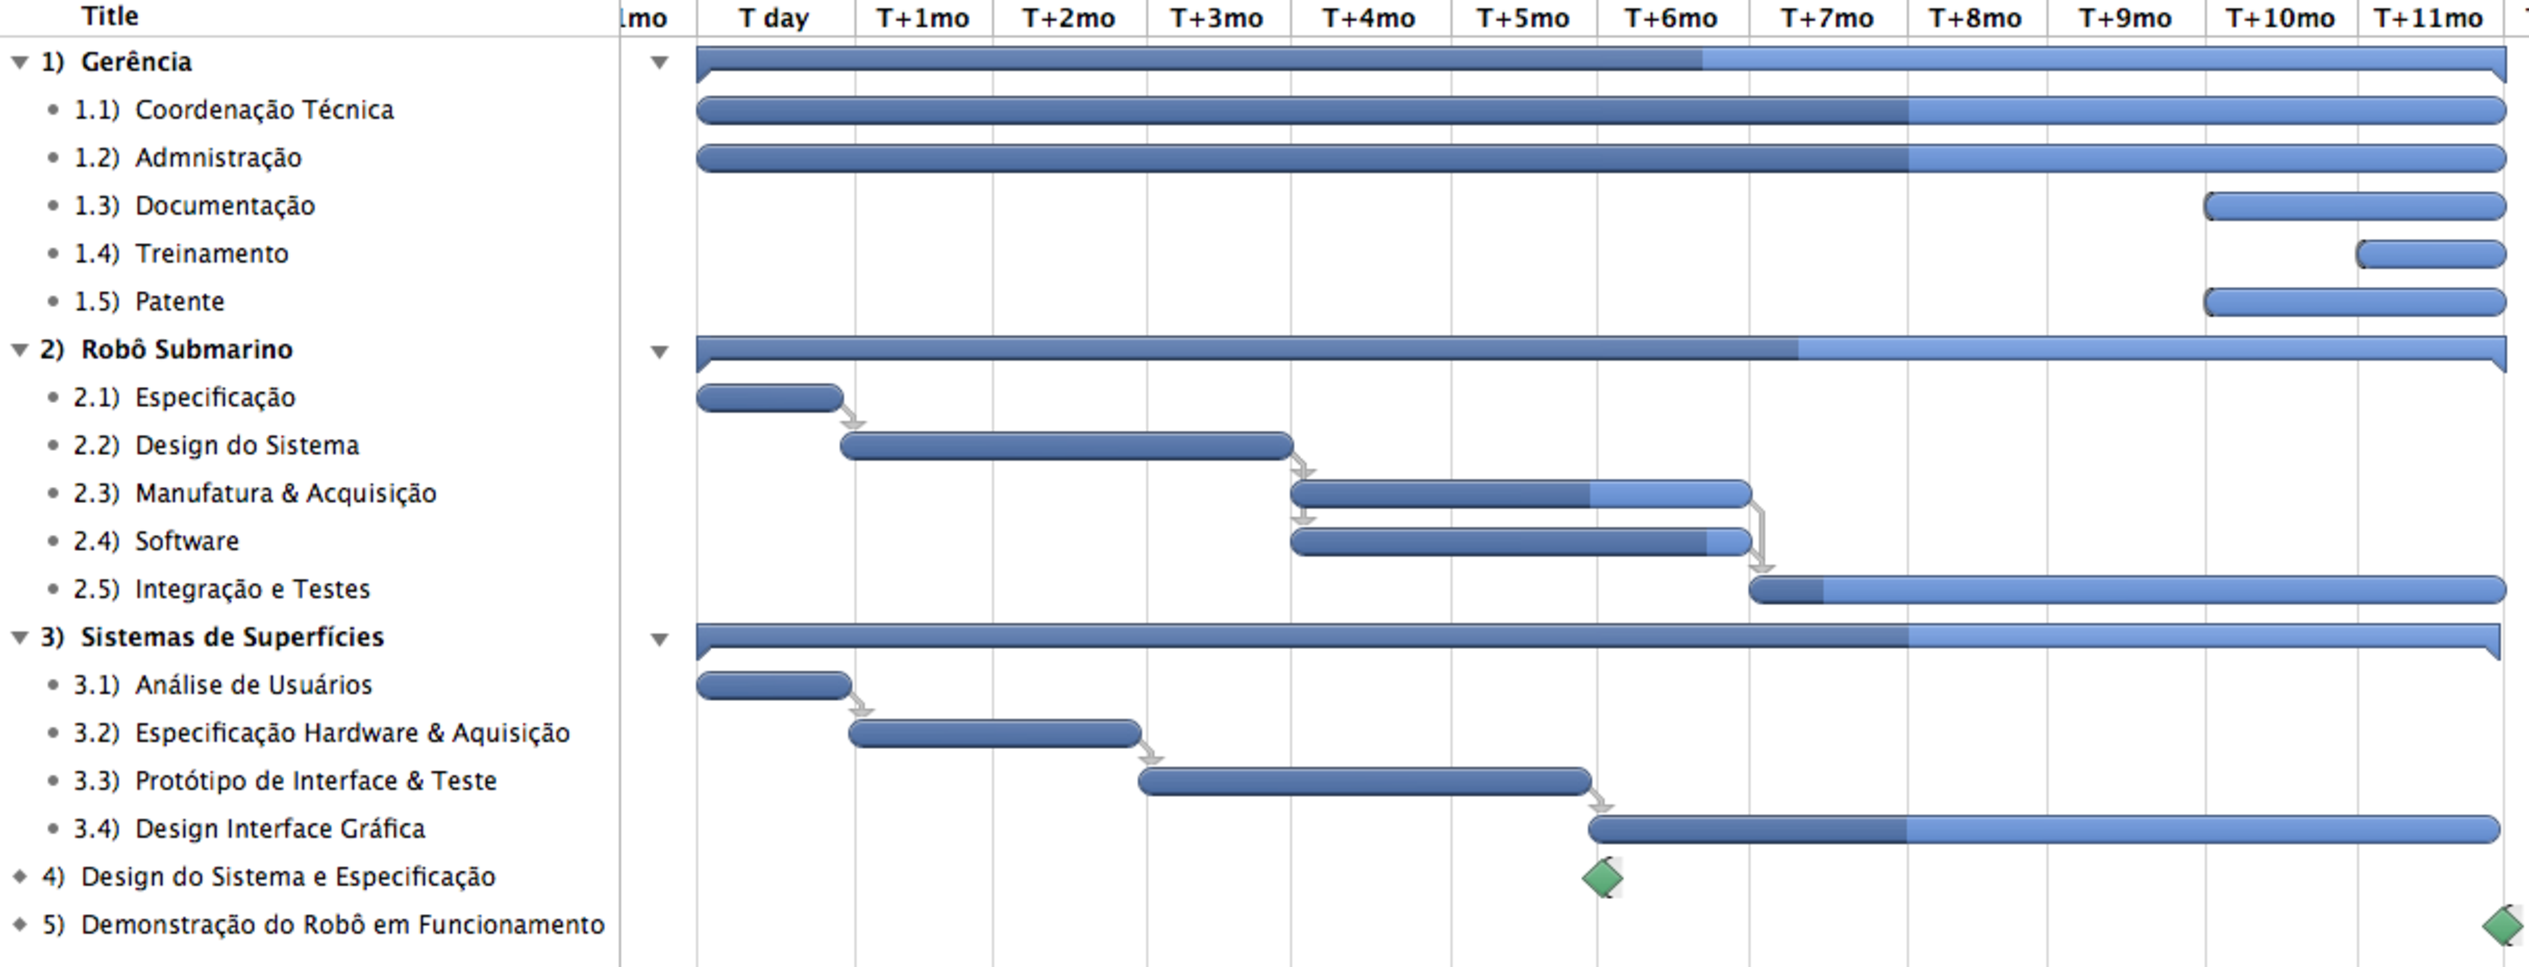
\includegraphics[angle=90,scale=0.55]{figs/gantt/Gantt.pdf}
\end{center}

\newpage%
{\bf  1) Ger�ncia}: O planejamento tecnol�gico e administrativo, organiza��o, coordena��o e controle utilizados para alcan�ar os objetivos gerais do projeto, que n�o est�o associados a hardware espec�fico ou elementos de software.

\begin{description}

\item[1.1) Coordena��o T�cnica]: Coordenar a parte t�cnica do projeto, atribuindo tarefas e revendo o trabalho conclu�do. O resultado da coordena��o t�cnica no per�odo e seus entreg�veis foram:

\begin{description}
	\item [Status] - Tarefa em andamento, sem atrasos.
	\item [Entreg�vel 01] - Atas de reuni�es de acompanhamento t�cnico e aloca��o de tarefas.
	\item [Entreg�vel 02] - Relat�rio Mensais 01, 02 e 03.
	\item [Entreg�vel 03] - Relat�rio Quadrimestral 01.
	\item [Entreg�vel 04] - Relat�rio Mensais 05, 06 e 07.
\end{description}


\item[1.2) Administra��o]:  Administrar a parte financeira do projeto. O resultado s�o as planilhas do balan�o financeiro do projeto atualizada

\begin{description}
	\item [Status] - Tarefa em andamento, sem atrasos.
	\item [Entreg�vel 01] - Relat�rio Mensais 01, 02 e 03.
	\item [Entreg�vel 02] - Relat�rio Quadrimestral 01.
	\item [Entreg�vel 02] - Relat�rio Quadrimestral 05, 06 e 07.
\end{description}


	\item[1,3) Documenta��o:] Este pacote de trabalho lida com a escrita da documenta��o t�cnica e de opera��es. Os resultados s�o os manuais e a documenta��o t�cnica do sistema.

\begin{description}
	\item [Status] - Tarefa n�o iniciada de acordo com o planejamento do projeto.
\end{description}

	\item[1,4) Treinamento:] Esfor�o necess�rio para treinar o pessoal de opera��o da hidrel�tricas no uso do  sistema rob�tico desenvolvido no projeto.

\begin{description}
	\item [Status] - Tarefa n�o iniciada.
\end{description}

	\item[1,5) Patente:] Solicita��o de patente de produto para o sistema rob�tico desenvolvido.

\begin{description}
	\item [Status] - Tarefa n�o iniciada de acordo com o planejamento do projeto.
\end{description}

\end{description}


\begin{description}

\vspace{0,5cm}

\item[ 2)  Rob� Submarino:] Este elemento lida com o trabalho necess�rio para desenvolver o sistema eletromec�nico do rob�.

\item[2,1) Especifica��o:] Neste pacote de trabalho, requisitos do sistema ser�o especificados atrav�s de reuni�es com os funcion�rios respons�veis pela opera��o na hidroel�trica e atrav�s de observa��es em campo. O resultado ser� um documento com os requisitos do sistema.

\begin{description}
	\item [Status] - Tarefa conclu�da.
	\item [Entreg�vel 01] - Documento de Projeto B�sico.
\end{description}

\item[2,2) Design do Sistema:] Processo de defini��o da arquitetura, componentes, m�dulos e interface que satisfazem os requisitos do sistema. O resultado ser� uma lista de componentes, arquitetura de software e projeto eletromec�nico do sistema.

\begin{description}
	\item [Status] - Tarefa atrasada, 2 meses. Atraso administrativo resultou em atraso na contrata��o das empresas de servi�os respons�veis pelo design da mec�nica e da arquitetura de software. 
	\item [Entreg�vel 01] - Relat�rio do Design Eletr�nico
\end{description}

\item[2,3) Manufatura e Aquisi��o:] Compra e constru��o dos componentes definidos durante a fase de design do sistema. O resultado ser�o as partes que integradas formar�o o rob�.

\begin{description}
	\item [Status] - Tarefa atrasada, 3 meses. Atraso na manufatura das partes mec�nicas. Raz�o: Os atrasos administrativos no projeto resultaram em atrasos na contrata��o do servi�o de especifica��o mec�nica.
\end{description}

\item[2,4) Software:] Desenvolvimento de drivers, controladores e comunica��o para o hardware do rob�. O resultado ser� uma biblioteca de componentes do software.

\begin{description}
	\item [Status] - Tarefa atrasada, 1,5 meses. Atraso na integra��o dos algoritmos em um �nico componente de software. Raz�o: Os atrasos administrativos no projeto resultaram em atrasos na contrata��o do servi�os de software
\end{description}

\item[2,5) - Integra��o e Teste:] Os componentes eletr�nicos, mec�nicos e de software ser�o integrado no sistema Viga Pescadora Inteligente. Este pacote de trabalho tamb�m inclui a instala��o e teste do sistema.

\begin{description}
	\item [Status] - Tarefa atrasada, 2 semanas. Testes de sensores foram realizados em Jirau pela equipe do projeto. Atraso na integra��o do sistema devido aos atrasos nos pacotes de trabalho de manufatura.
\end{description}

\end{description}

\begin{description}

\item[3) Sistemas de Superf�cie:] Este elemento inclui o hardware e o software necess�rios para a opera��o do rob� na superf�cie, incluindo a concep��o, desenvolvimento, implementa��o e integra��o da comunica��o, interface e ger�ncia de dados.

\item[3,1) An�lise de Usu�rio:] An�lise dos potenciais usu�rio do sistemas. Este pacote de trabalho vai resultar em um documento que define: O que o usu�rio espera do sistema. Como o sistema ir� fazer parte do dia a dia da opera��o. Qual � a capacita��o t�cnica do futuro usu�rio. Qual apar�ncia de interface t�m um maior apelo para o usu�rio.

\begin{description}
	\item [Status] - Tarefa conclu�da.
	\item [Entreg�vel 01] - Documento de An�lise de Usu�rio.
\end{description}

\item[3,2) Especifica��o de Hardware e Aquisi��o:] Este pacote de trabalho inclui a especifica��o e aquisi��o do equipamento necess�rio para operar o rob� a partir da superf�cie. O resultado � um lista de componentes, e respectivos fabricantes, a serem comprados para o projeto.

\begin{description}
	\item [Status] - Tarefa conclu�da
	\item [Entreg�vel 01] - Relat�rio de especifica��o de hardware.
\end{description}


\item[3,3) Prot�tipo de Interface e Teste:] Desenvolvimento de telas interativas simples, sem conte�do, concentrando apenas no desenvolvimento da parte visual da interface. Estes prot�tipo de interface vai ser testado com os futuros usu�rio dos sistema e o resultado da sensa��o da mesma ser� avaliada.

\begin{description}
	\item [Status] - Tarefa iniciada, viagem para an�lise do prot�tipo de interface com o operador de p�rtico rolante realizada, finalizando a escrita do relat�rio da intera��o. 
\end{description}

\item[3,4) Interface de Usu�rio:] Implementa��o da interface de usu�rio (GUI) do rob�, o que permite a visualiza��o e o seu controle. O resultado ser� um software.

\begin{description}
	\item [Status] - Tarefa iniciada. Implementa��o inicial sem conte�do do prot�tipo de interface em um Tablet Android.
\end{description}

\end{description}

%%******************************************************************************
%% SECTION - Financeiro
%%******************************************************************************
\section{Financeiro}
\label{financeiro}

O relat�rio financeiro aqui apresentado t�m como objetivo demonstrar o que foi estimado no in�cio do projeto, o que foi at� o momento executado e a previs�o atual dos gastos at� o fim do projeto, fornecendo uma vis�o global do plano financeiro do projeto. Logo, as informa��es contidas neste  relat�rio ser�o diferentes das informa��es contidas no relat�rio financeiro de presta��o de contas, o qual detalha apenas os lan�amentos realizados na conta do projeto at� a data de fechamento do m�s. Por favor, notar que existem itens detalhados como executados neste relat�rio que n�o estar�o presentes na presta��o de contas. Isto ocorre devido a defasagem de tempo entre a decis�o de comprar o item e a data de pagamento da nota fiscal. Por mais, todos as informa��es presentes em ambos os relat�rios dever�o ser consistentes e em caso de inconsist�ncia o valor relatado no relat�rio de presta��o de contas dever ser considerado como o correto.

\subsection{Planilha de desembolso}

\begin{center}
  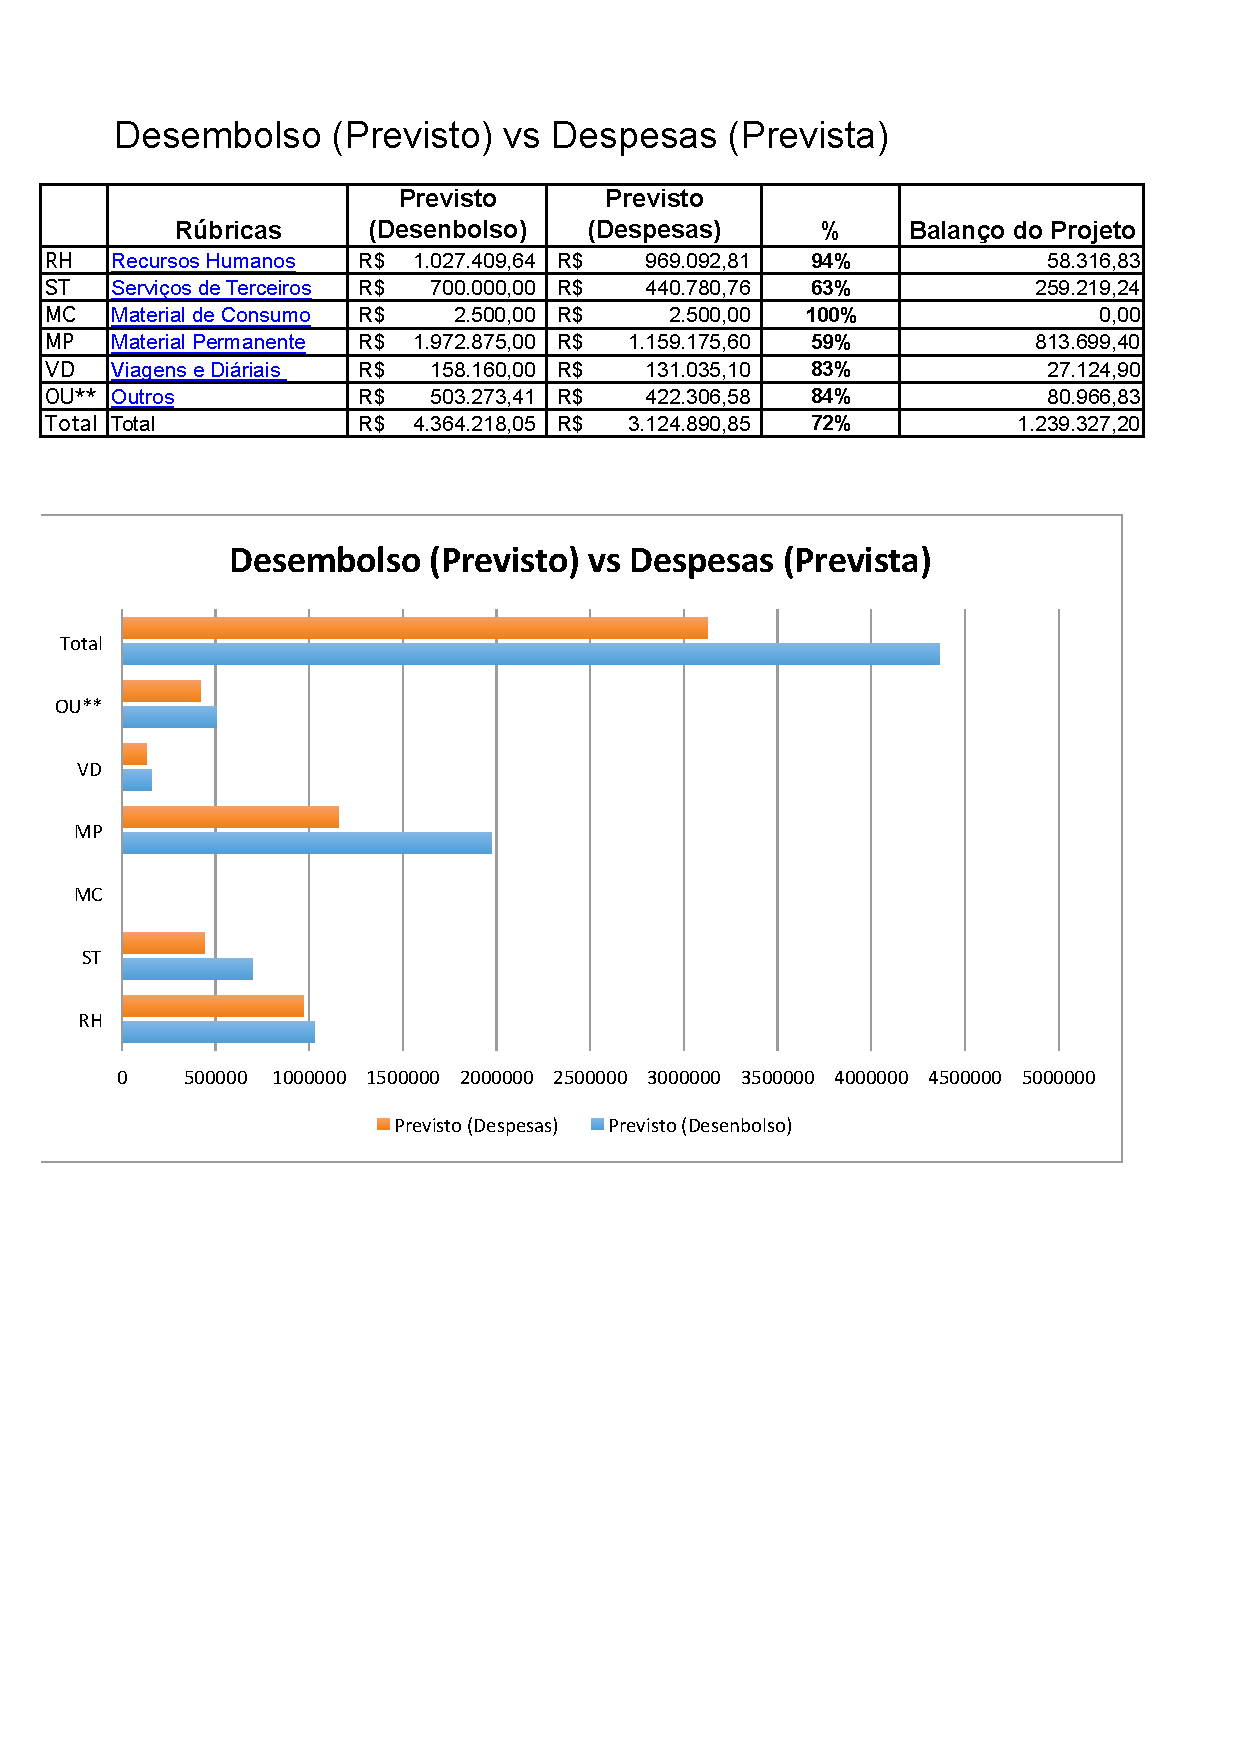
\includegraphics[width=\textwidth]{figs/financeiro/Balanco.pdf}
\end{center}

\subsection{Recursos humanos}

\begin{center}
  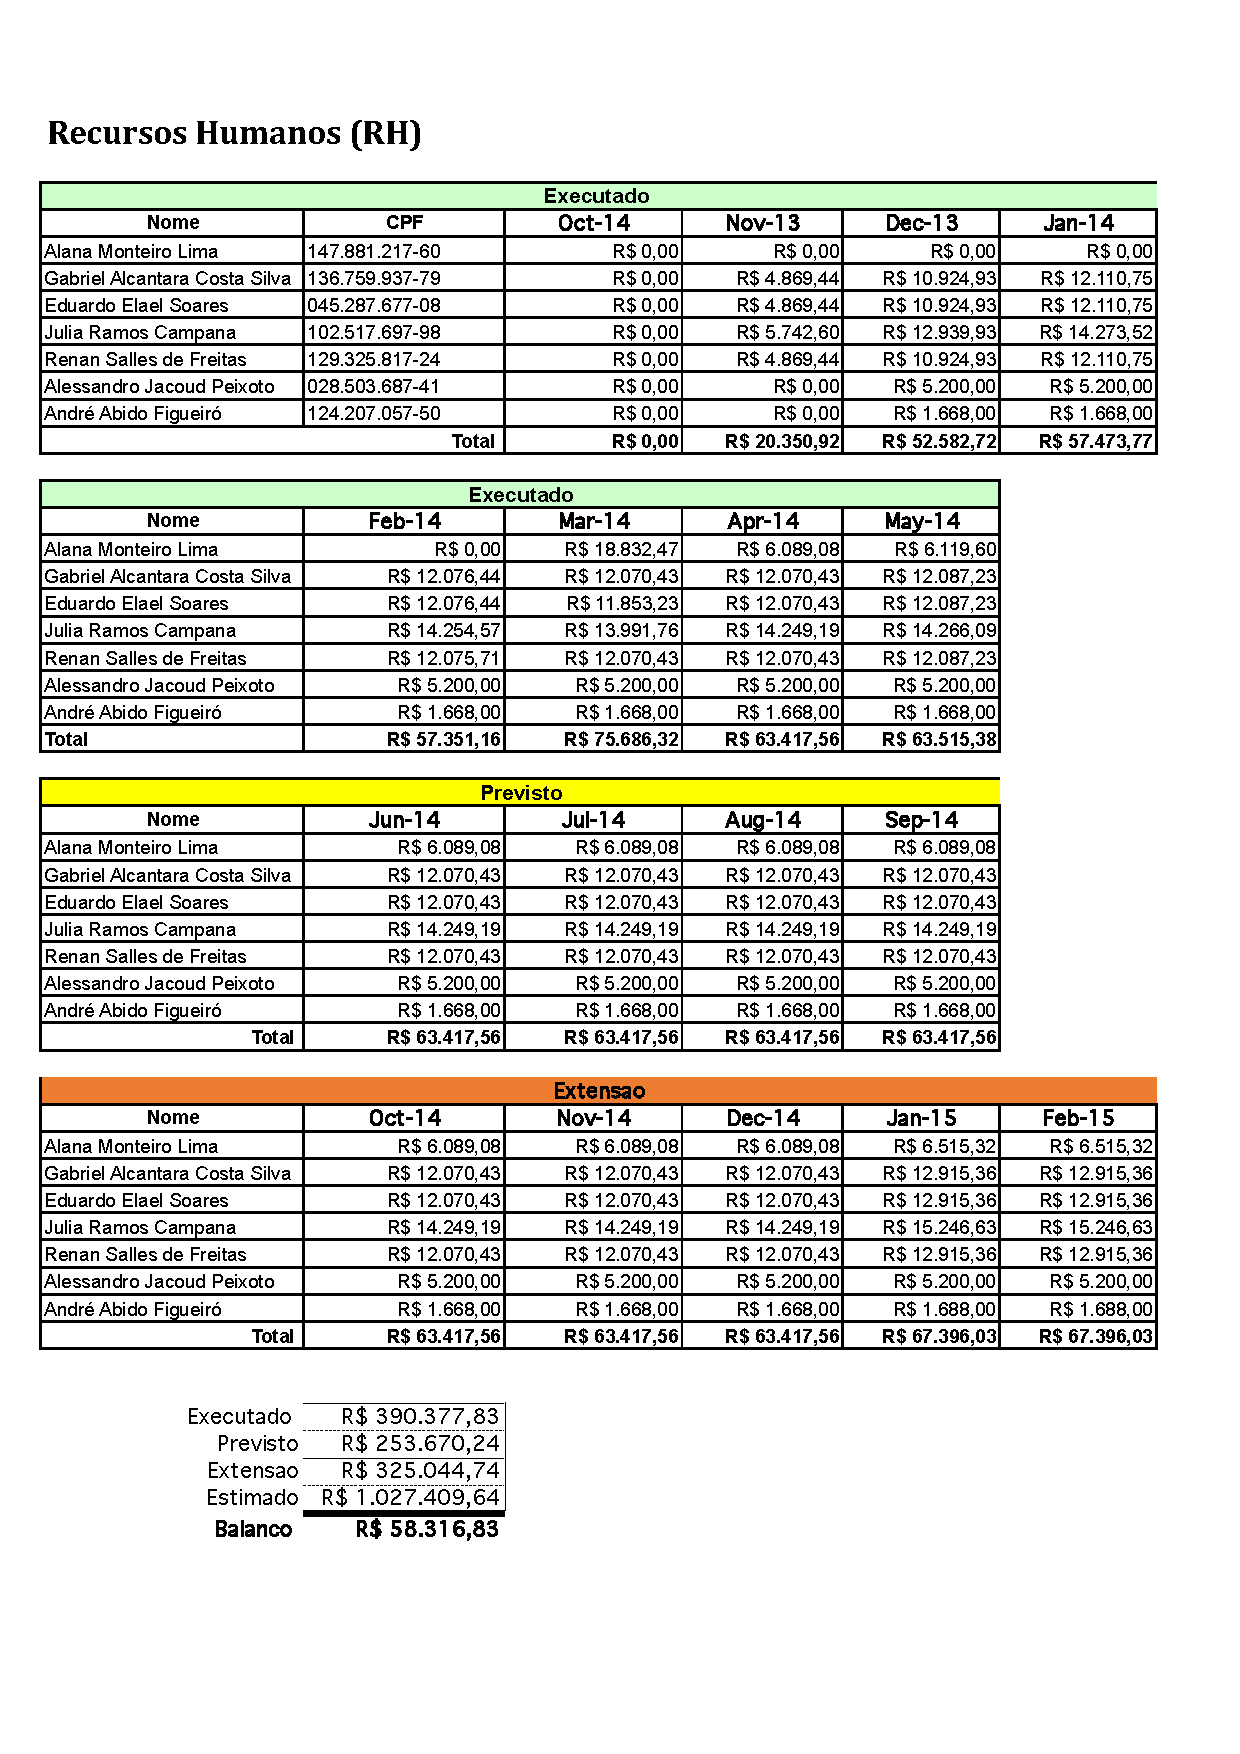
\includegraphics[width=1\columnwidth]{figs/financeiro/RH.pdf}
\end{center}

\subsection{Servi�os de terceiros}

\begin{center}
  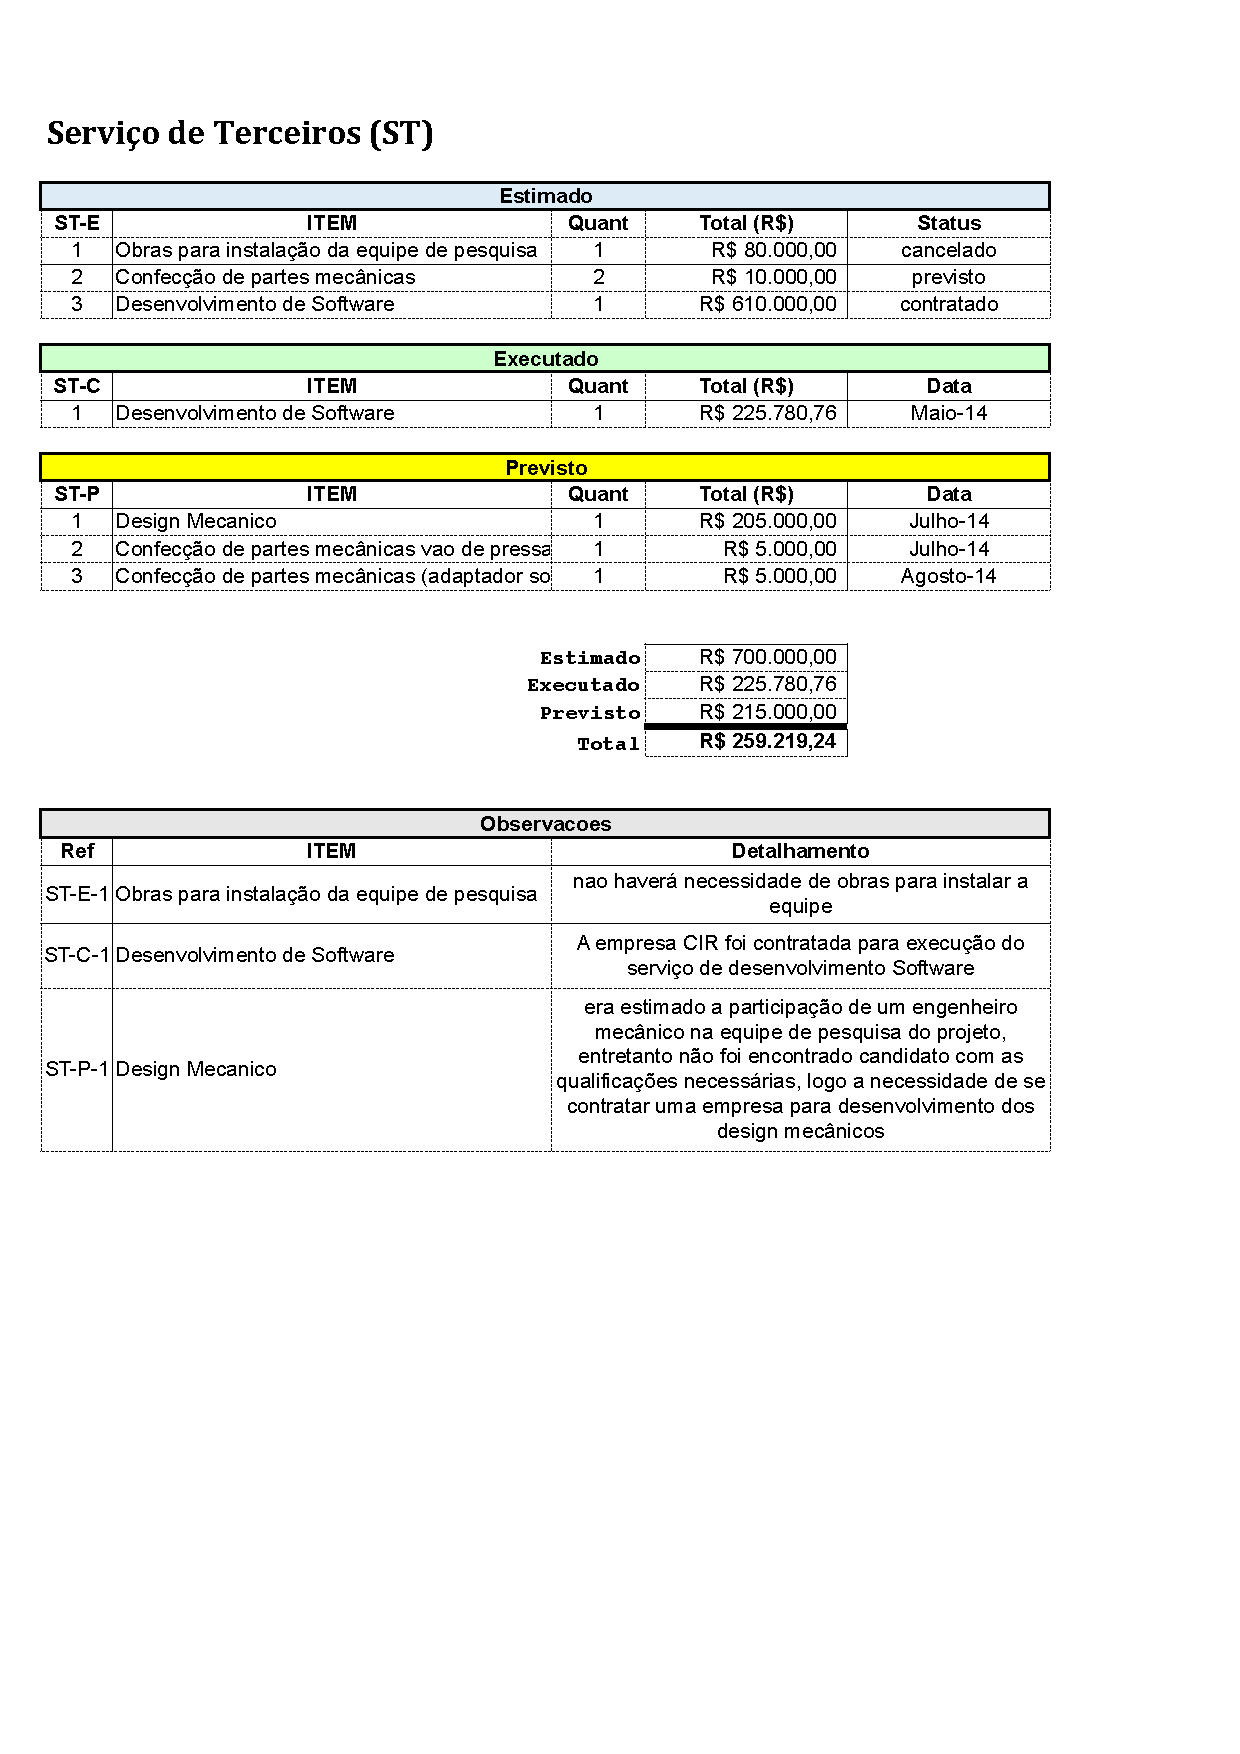
\includegraphics[width=1\columnwidth]{figs/financeiro/ST.pdf}
\end{center}

\subsection{Material de consumo}

\begin{center}
  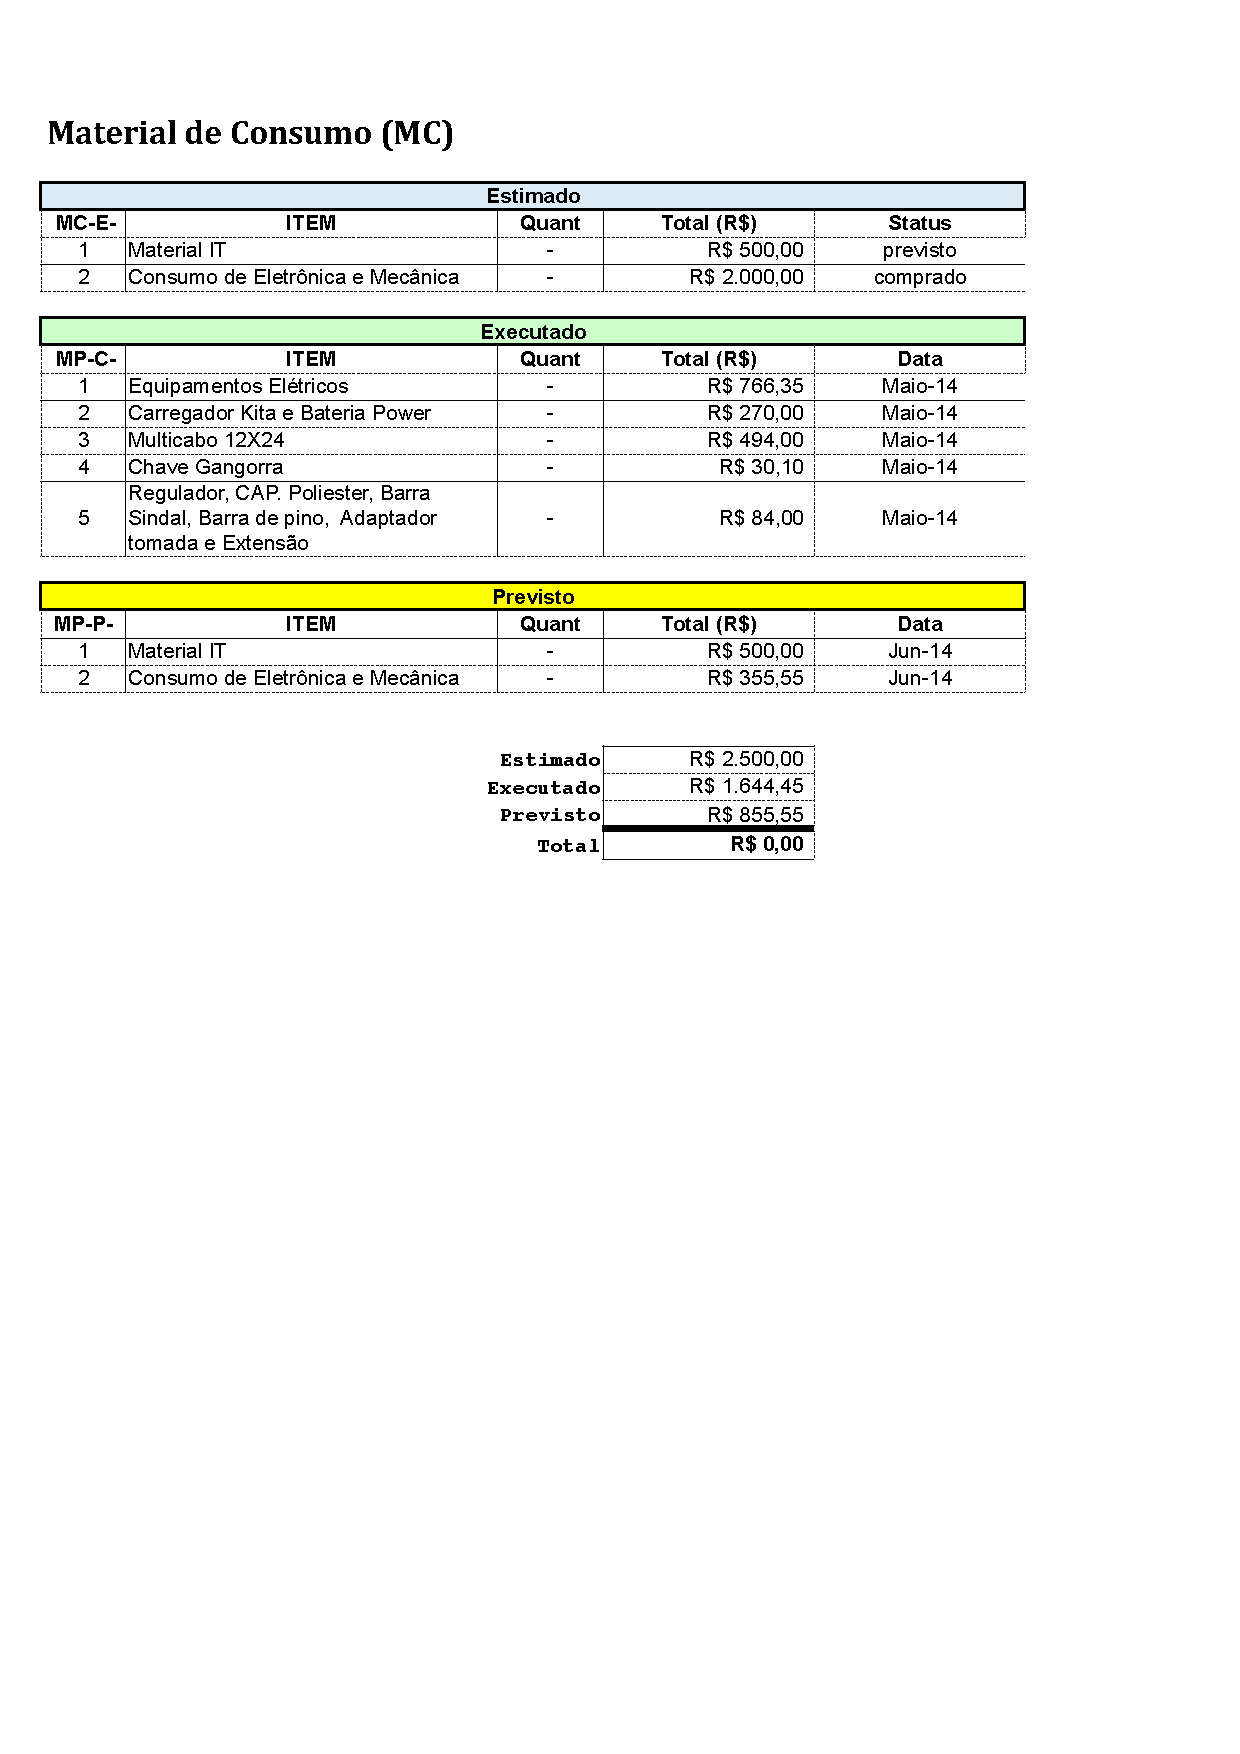
\includegraphics[width=1\columnwidth]{figs/financeiro/MC.pdf}
\end{center}

\subsection{Material permanente}

\begin{center}
  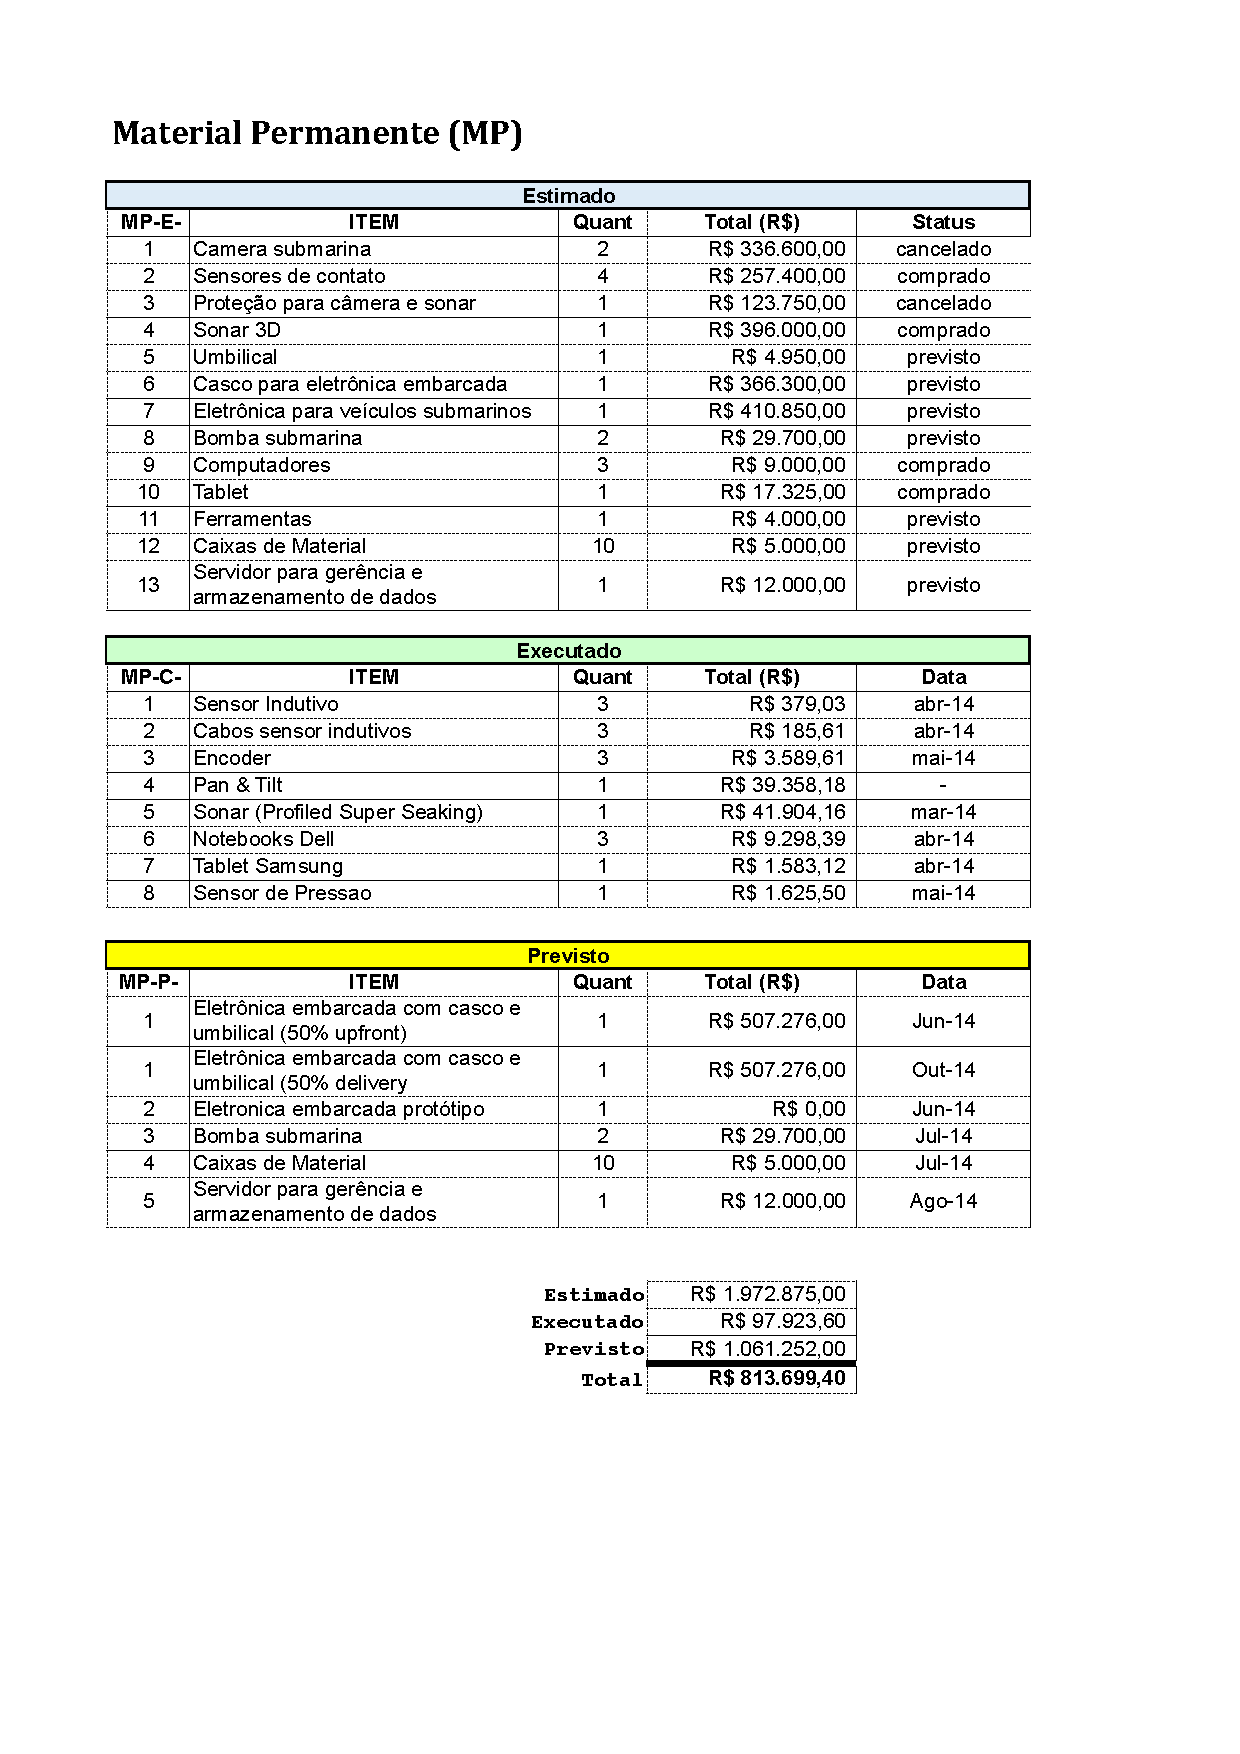
\includegraphics[width=1\columnwidth]{figs/financeiro/MP.pdf}
\end{center}

\begin{center}
  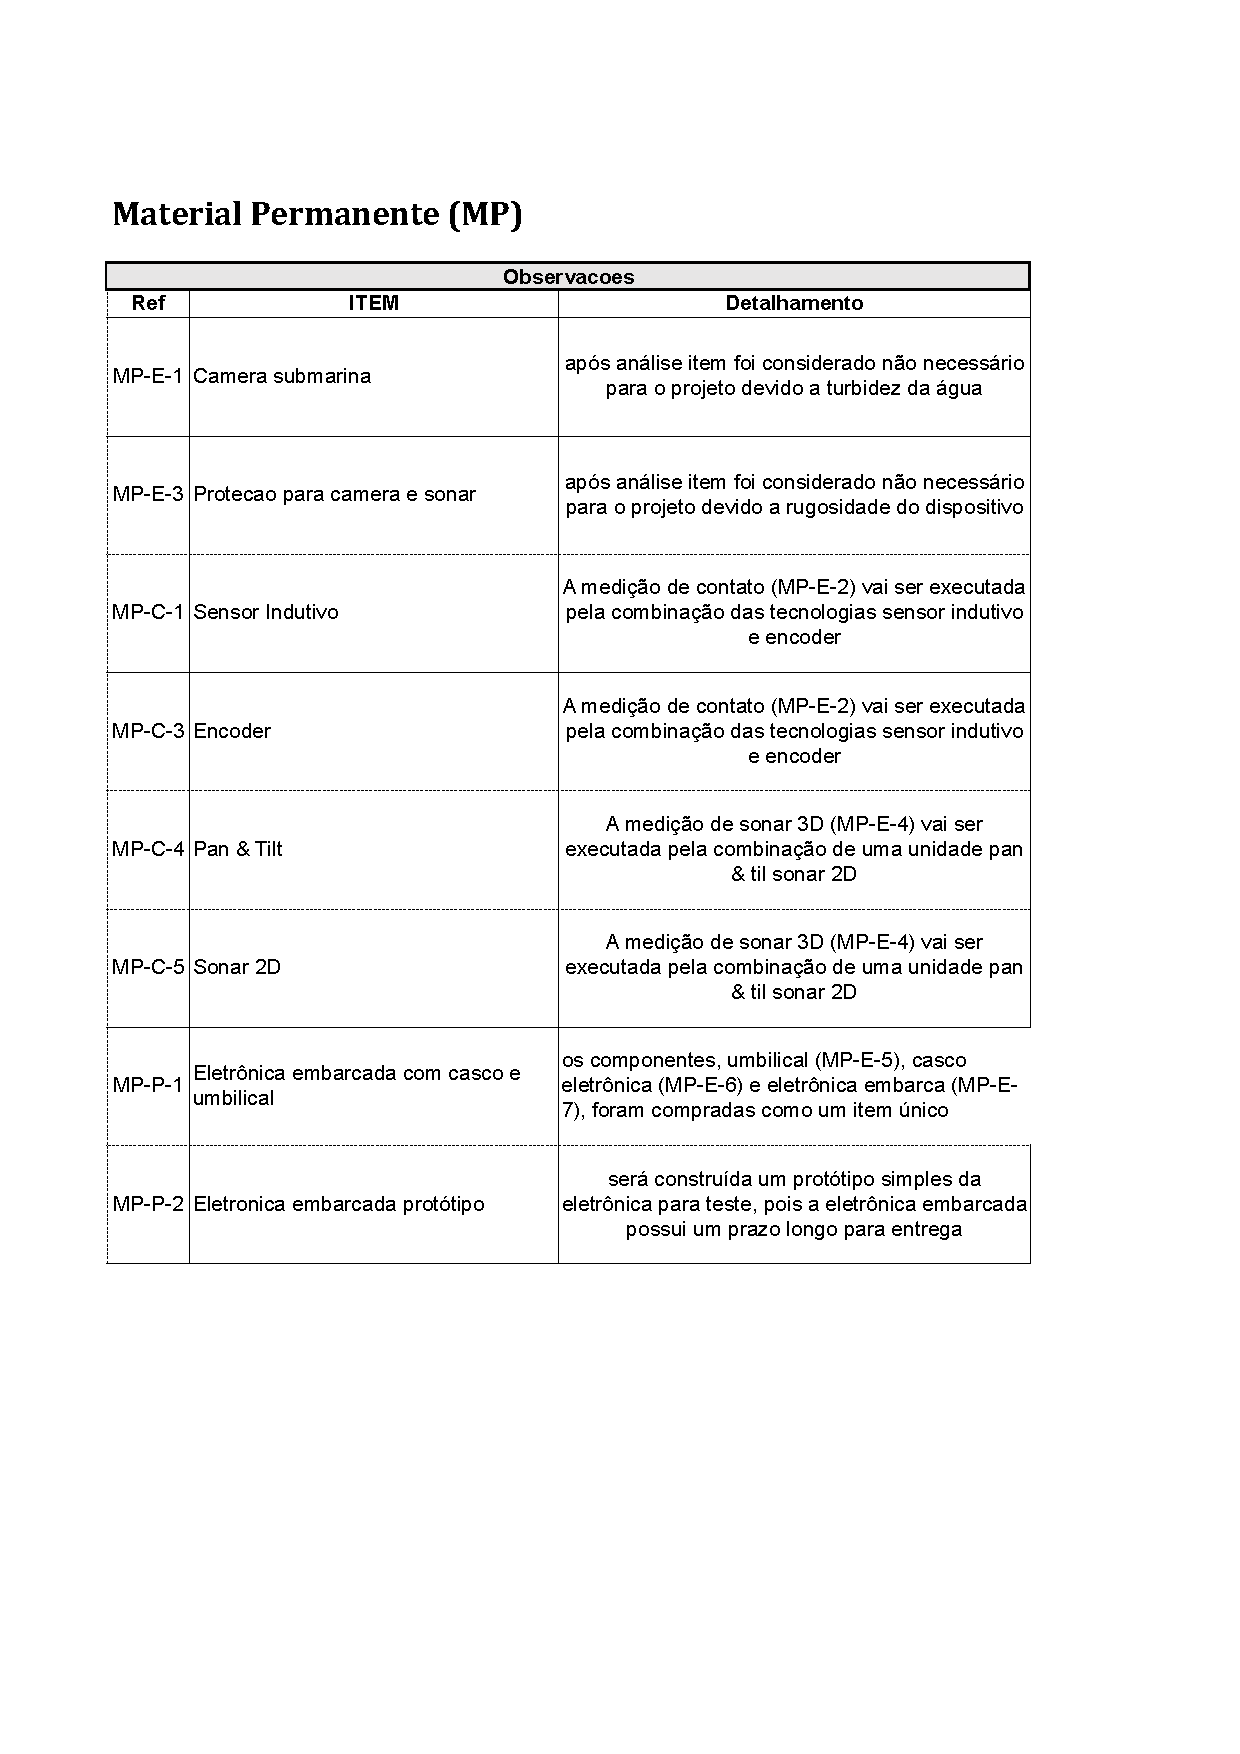
\includegraphics[width=1\columnwidth]{figs/financeiro/MP_Detalhamento.pdf}
\end{center}
\subsection{Viagens e di�rias}

\begin{center}
  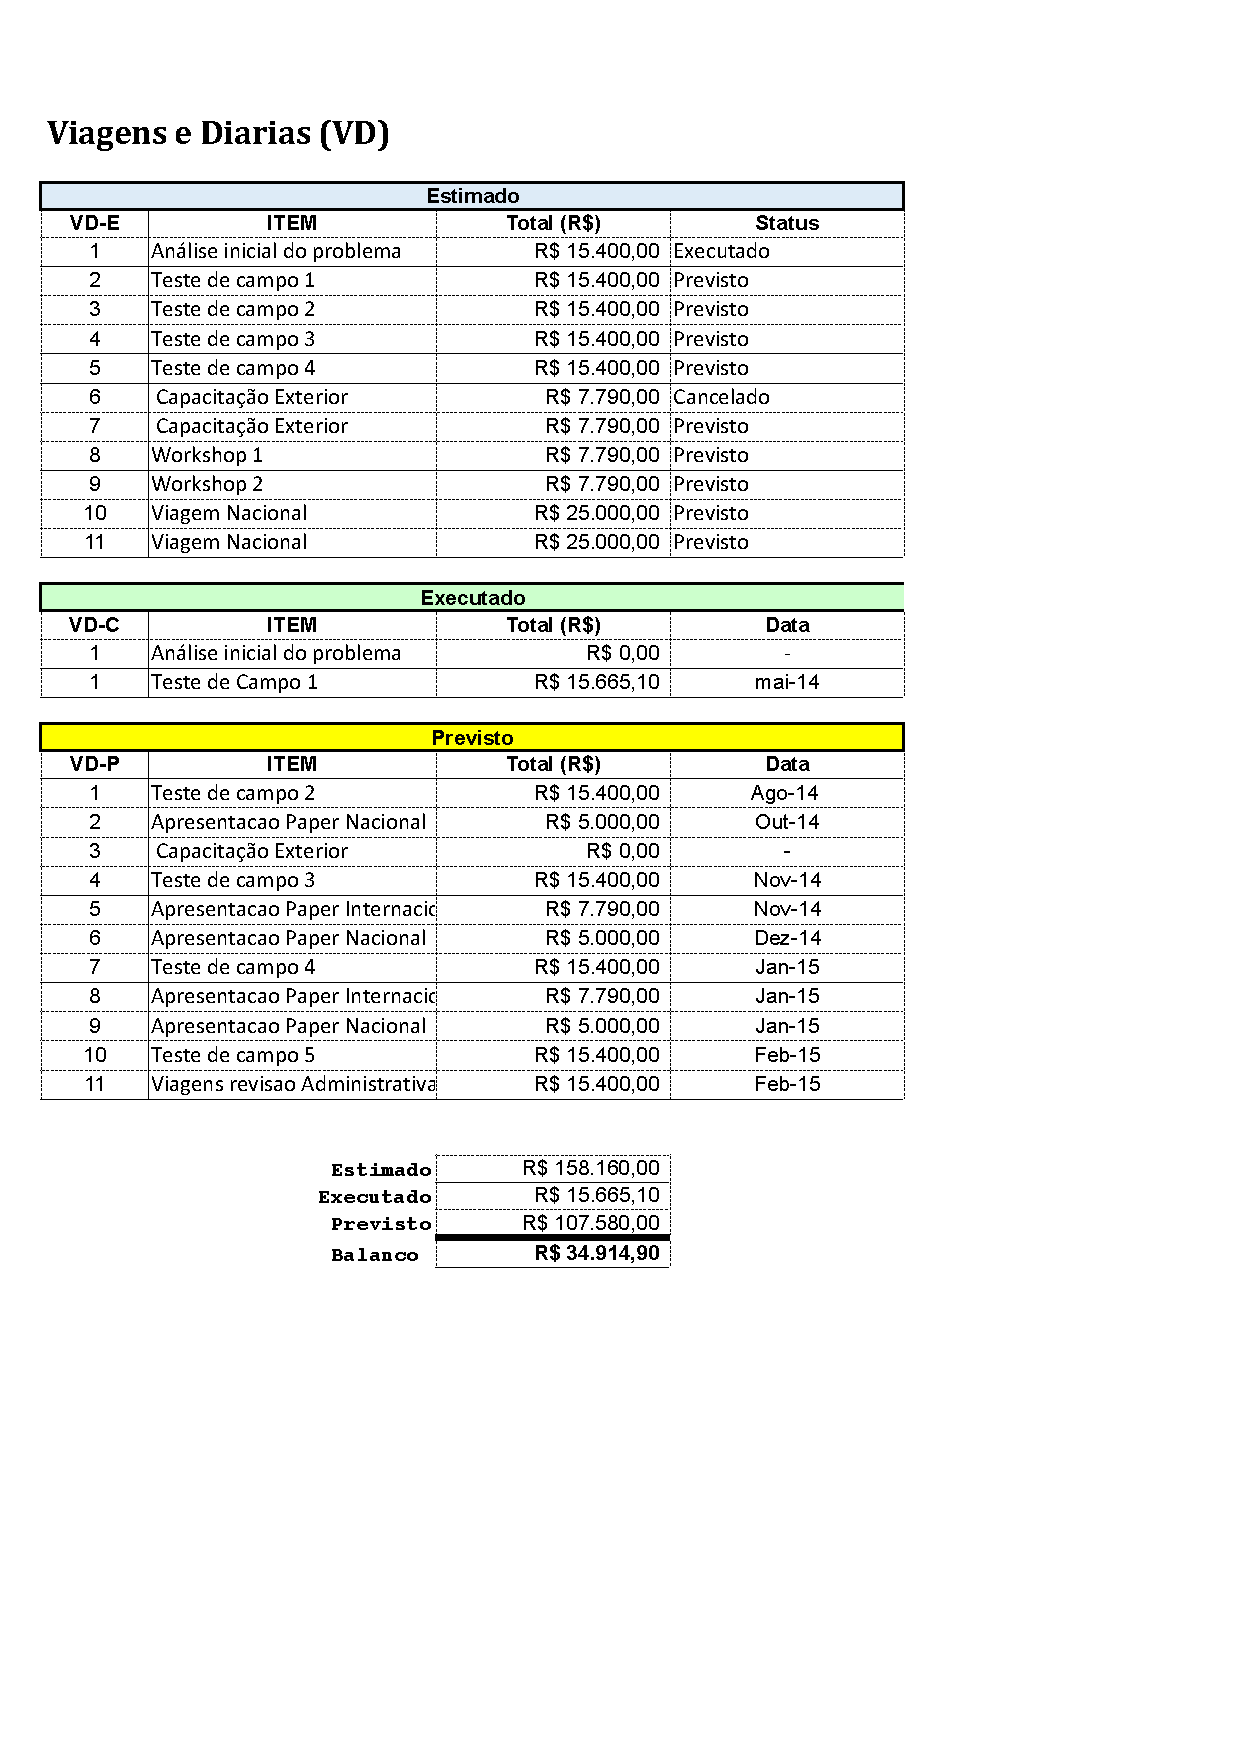
\includegraphics[width=1\columnwidth]{figs/financeiro/VD.pdf}
\end{center}

\subsection{Outros}

\begin{center}
  \includegraphics[width=1\columnwidth]{figs/financeiro/OU.pdf}
\end{center}











%%******************************************************************************
%% SECTION - C�lculos e modelagens;
%%******************************************************************************
\setcounter{secnumdepth}{3}
\section{C�lculos e modelagens}
\label{calculos_e_modelagens}

Neste quadrimestre, foi desenvolvida a modelagem do sistema de carga e descarga de baterias referente � tese de mestrado do bolsista Andr� Figueir� (vide anexo \ref{App:AppendixModelagemBateria}).

%%******************************************************************************
%% SECTION - Resultados alcan�ados (resumo de medidas efetuadas, resultados de an�lises e ensaios, especifica��es de prot�tipos, etc.);
%%******************************************************************************

\setcounter{secnumdepth}{3}
\section{Resultados alcan�ados}
\label{resultados_alcancados}

\subsection{Eletr�nica}

A partir da primeira solu��o conceitual para a eletr�nica, foram projetadas duas PCBs. Para o projeto, utilizou-se o software Altium, que permite gerar esquem�ticos e modelos 3D com roteamento. Uma das placas tem como objetivo garantir robustez atrav�s de redund�ncia de micro controladores, enquanto que a outra foca em simplicidade, entrega r�pida e de menor custo. Alguns componentes da placa j� est�o dispon�veis em laborat�rio e foram testados, outros est�o na lista de componentes que ser�o adquiridos ainda at� fim de maio.

A segunda solu��o para a eletr�nica embarcada, que envolve a utiliza��o de um PC, resultou na pesquisa de fornecedores de PC104 com placas ADC e CAN. Drivers de diversos dispositivos j� est�o dispon�veis em ROCK, o que facilita a execu��o desta solu��o tanto para software quanto para hardware.
Por �ltimo, em Maio, foi montado um prot�tipo da eletr�nica embarcada para os testes em Jirau. Ser�o utilizadas as interfaces RS232-USB e anal�gica para os testes do sonar Micron (dispon�vel em laborat�rio) e sensores indutivos. A alimenta��o ser� realizado por um pack de baterias 12V, 7Ah em s�rie. A proposta de solu��es para a arquitetura da eletr�nica do projeto ROSA encontra-se no Relat�rio de Eletr�nica.

 \begin{figure}[ht!]
    \centering 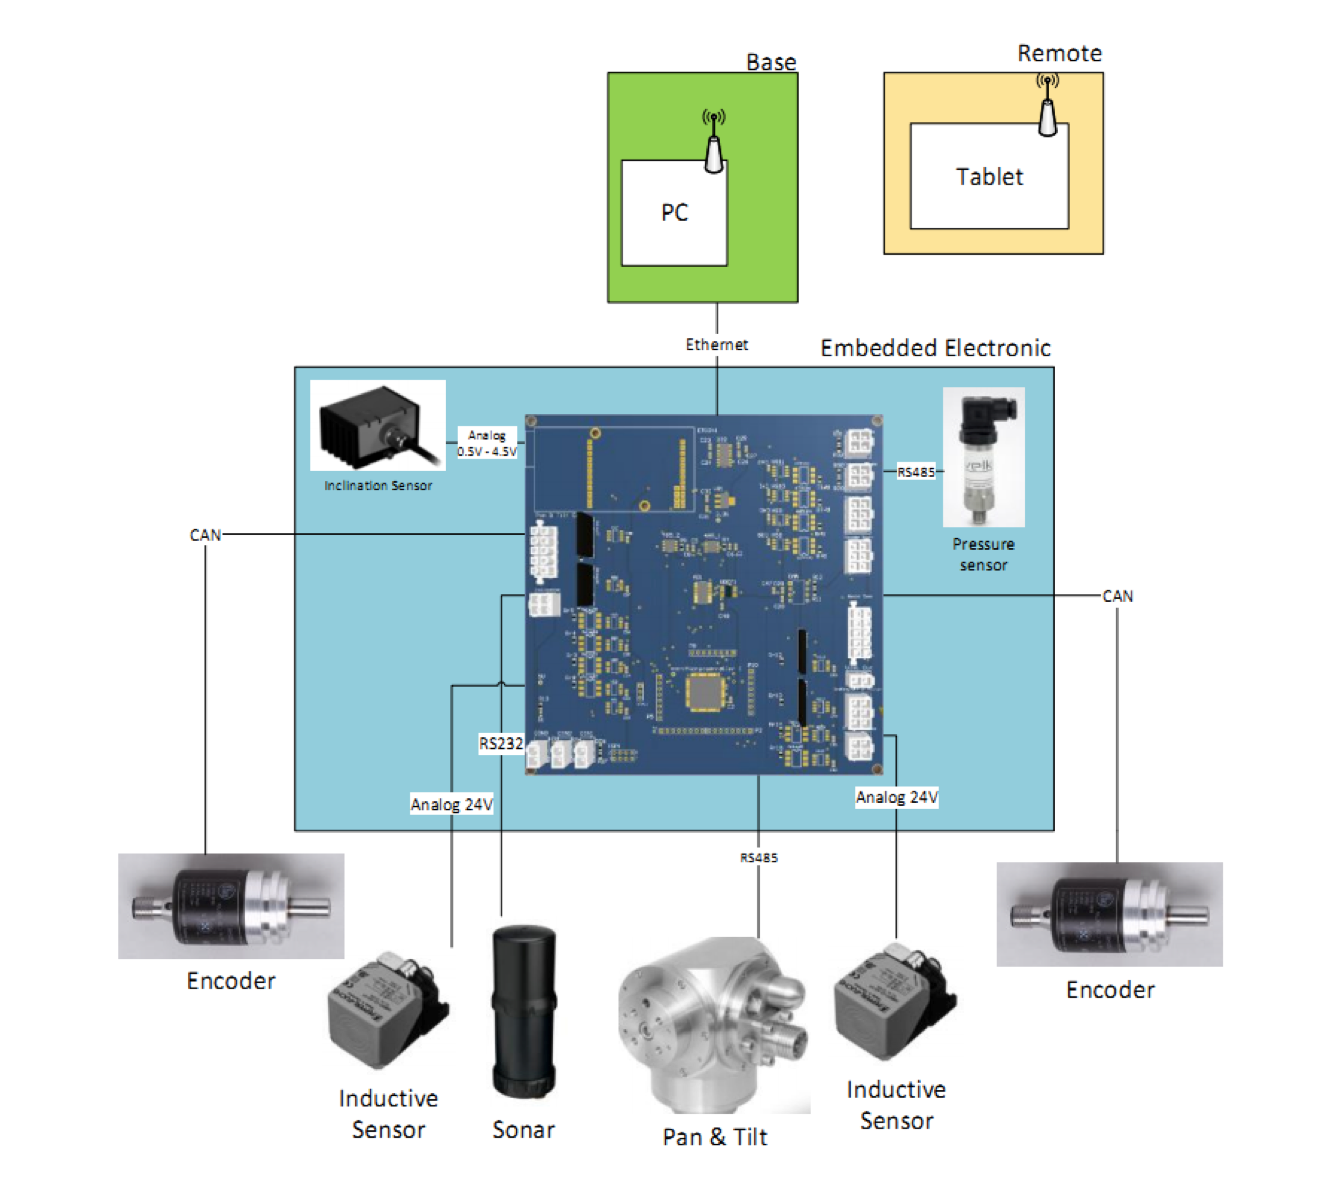
\includegraphics[width=12cm]{figs/resultados/eletronica}
    \caption{Diagrama da eletr�nica.}
    \label{fig:eletronica}
\end{figure}

\subsection{Reconstru��o 3D por sonar}

O princ�pio por tr�s da parte de reconstru��o 3D do projeto �  acumular os dados provenientes do sonar em uma representa��o volum�trica. Esse ac�mulo ajuda a resolver o problema de ambiguidade dos dados de sonar. O framework Octomap foi definido durante a fase de defini��o do projeto como a biblioteca a ser utilizada para o ac�mulo volum�trico. Logo, o Octomap foi integrado ao framework Robot Construction Kit (ROCK), framework de rob�tica utilizado no projeto. A integra��o foi testada em laborat�rio utilizando-se um sonar Tritech Micron. A figura \ref{fig:octomap} ilustra o preenchimento volum�trico de acordo com a forma de onda proveniente do sonar e a intensidade de reflex�o.

\begin{figure}[ht!]
    \centering 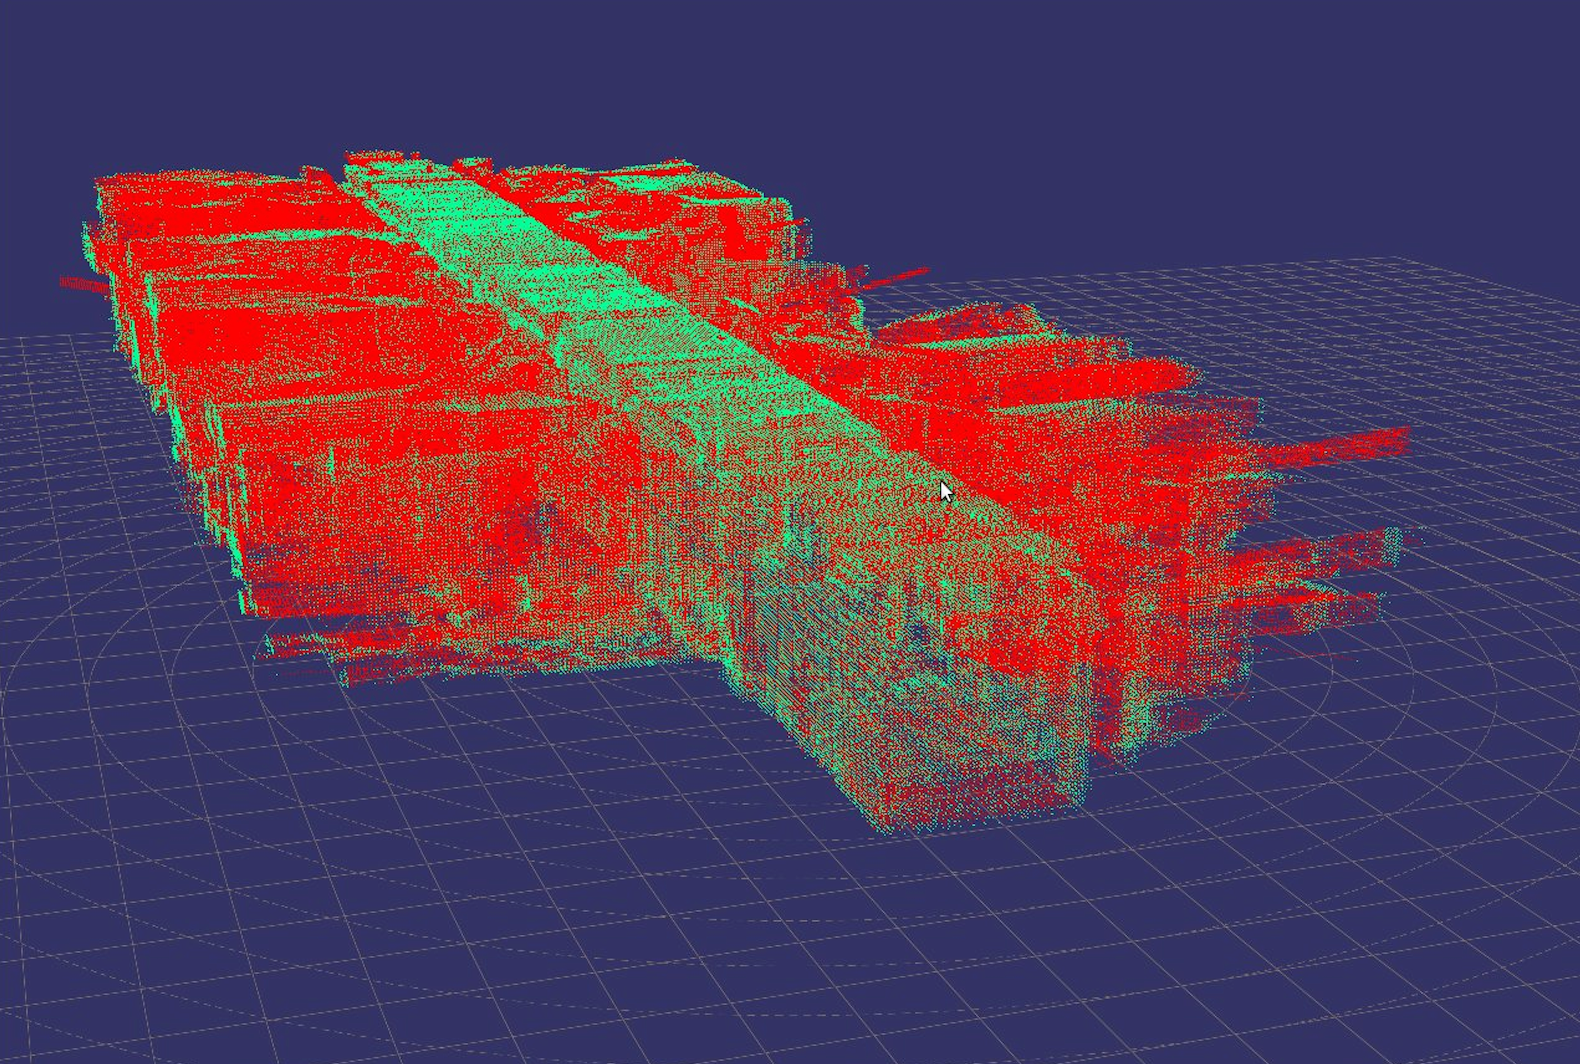
\includegraphics[width=12cm]{figs/resultados/octomap}
    \caption{Octomap}
    \label{fig:octomap}
\end{figure}

\subsection{Interface}

A interface com o usu�rio facilita a utiliza��o do rob� ROSA, permitindo a compreens�o das informa��es geradas pelo rob� de modo intuitivo.
Neste quadrimestre, o prot�tipo da interface foi desenvolvido e implementado em um tablet Android para an�lise de usabilidade, como ilustrado na figura \ref{fig:userinterface}.

A prototipagem � uma t�cnica de an�lise interativa em que os usu�rios est�o ativamente envolvidos no desenvolvimento da interface.
A descri��o detalhada do prot�tipo de interface encontra-se no Relat�rio de Interface de Usu�rio.

\begin{figure}[ht!]
    \centering 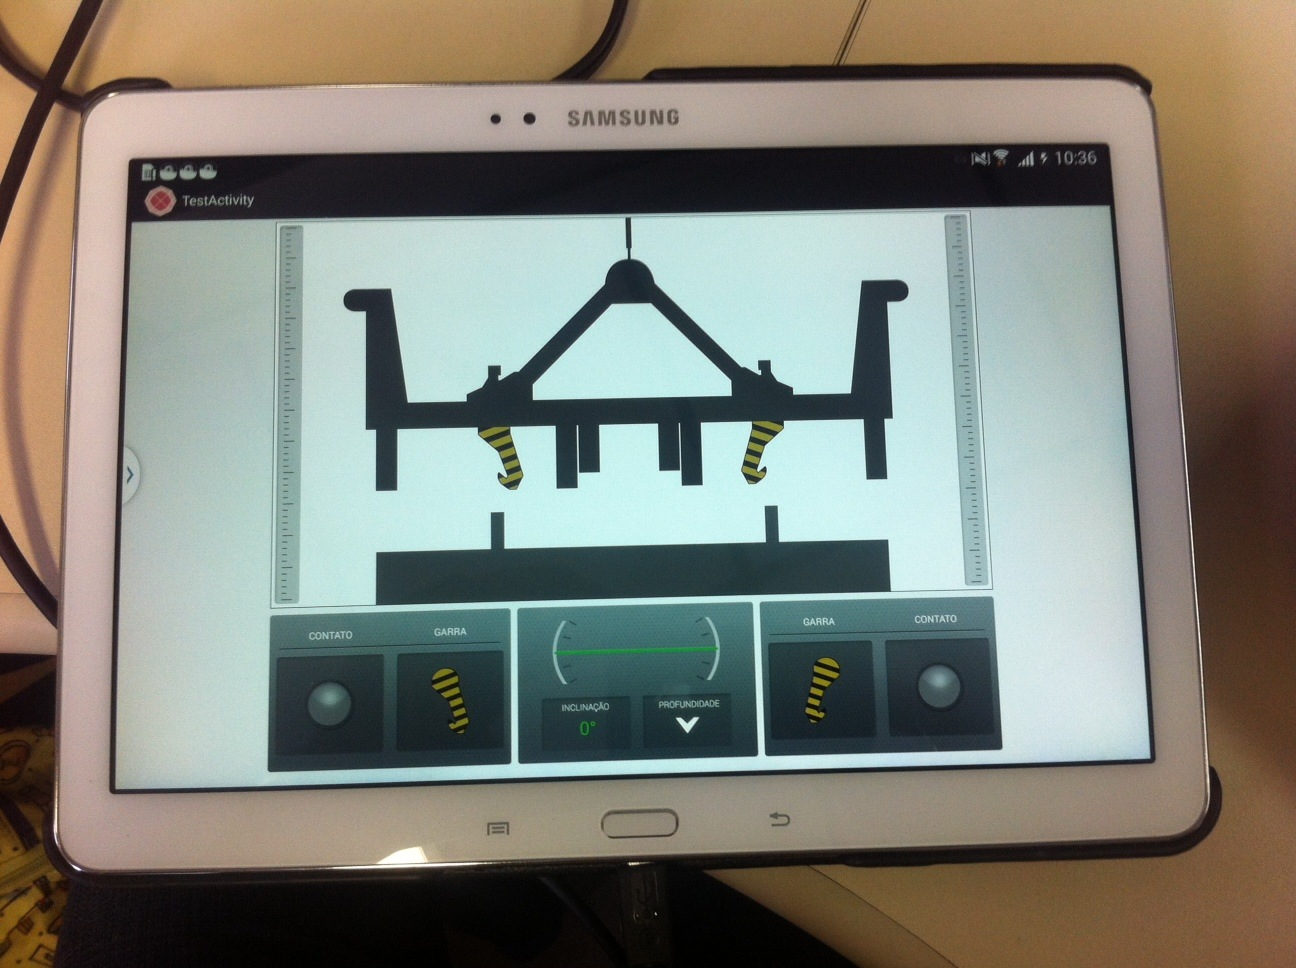
\includegraphics[width=12cm]{figs/resultados/UI}
    \caption{Interface Usu�rio}
    \label{fig:userinterface}
\end{figure}

\subsection{Drivers}

Os drivers permitem a comunica��o entre o computador e os devices conectados ao mesmo.
Neste quadrimestre, foram encomendados os sensores especificados no projeto b�sico. Dentre eles, somente o sensor indutivo, encoder e profund�metro foram entregues.
Os drivers para os dispositivos entregues foram desenvolvidos e integrando ao Framework de rob�tica ROCK.
A comunica��o e funcionalidade dos dispositivos foram testados em bancada como ilustrado na figura \ref{fig:teste_bancada}.

\begin{figure}[ht!]
    \centering 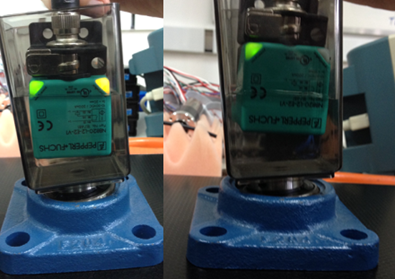
\includegraphics[width=12cm]{figs/resultados/teste_bancada.png}
    \caption{Tese de Bancada do Sensor Indutivo}
    \label{fig:teste_bancada}
\end{figure}




%%******************************************************************************
%% SECTION - Descri��o sum�ria da metodologia adotada no desenvolvimento das etapas;
%%******************************************************************************
\setcounter{secnumdepth}{3}
\section{Metodologia}
\label{metodologia}

\subsection{Defini��o}

Ap�s a an�lise e compreens�o do problema de inser��o e remo��o de Stoplogs em
visita de campo, foi feita uma \textbf{Pesquisa Bibliogr�fica} e um \emph{brainstorm} com o objetivo de alcan�ar um conceito s�lido de solu��o ao problema.

A partir do resultado dessa pesquisa foi desenvolvido um conceito base de solu��o rob�tica, descrito na se��o {\bf Escopo} do projeto b�sico. Baseado neste conceito, foram realizadas pesquisas de tecnologias e de fornecedores (se��o  {\bf Pesquisa Tecnol�gica} do projeto b�sico) de forma recursiva e convergente com rela��o aos resultados. Isto
�, com base nas pesquisas de solu��o tecnol�gicas poss�veis, buscam-se fornecedores compat�veis e com o
resultado e informa��o dos produtos dos fornecedores encontrados faz-se
novamente uma pesquisa de tecnologia, agora mais aprofundada, e assim sucessivamente
at� que seja encontrado um resultado final satisfat�rio.

Esta pesquisa � focada nos componentes a serem utilizados. Dessa maneira, a escolha dos fornecedores � justificada n�o somente na conformidade t�cnica, mas tamb�m no tempo de entrega,
dificuldade de importa��o, suporte e reconhecimento. O escopo inicial de solu��o
� ent�o atualizado e detalhado de acordo com o resultado desta pesquisa, resultando na descri��o do rob� a ser constru�do no projeto.

\subsection{Execu��o}

Na segunda etapa, as defini��es encontradas na primeira etapa s�o executadas:
Os materiais especificados foram requisitados pelo administrativo do projeto aos respectivos fabricantes definidos.
Os algoritmos definidos foram implementadas no framework de rob�tica do projeto pela equipe de desenvolvimento.
A interface gr�fica foi prototipada e a compreens�o do fluxo de informa��o testada com o usu�rio final.



%%******************************************************************************
%% SECTION - Reuni�es, palestras e cursos realizados (internos e externos);
%%******************************************************************************

\section{Reuni�es, palestras e cursos}
\label{reunioes_palestras_e_cursos}

As reuni�es de acompanhamento do projeto no quadrimestre foram realizadas nas datas listadas abaixo (vide atas no anexo \ref{Atas}):

\begin{itemize}
	\item 3, 14, 18 e 24 de Fevereiro 2014.
	\item 11 de Marco de 2014.
	\item 4, 14 e 29 de Abril 2014.
	\item 6 e 15 de Maio de 2014.
\end{itemize}




%%******************************************************************************
%% SECTION - Viagens Realizadas
%%******************************************************************************
\setcounter{secnumdepth}{3}
\section{Viagens}

Nenhuma viajem foi realizada no quadrimestre.



%%******************************************************************************
%% SECTION - Apresentar outras informações relevantes. Por exemplo, o recebimento de prêmios;
%%******************************************************************************

\section{Outros}
\label{outros}

Nenhuma outra informa��o relevante no quadrimestre.
\newpage
\appendix
%\section{Anexos} \label{Anexos}
%
%Seguem em anexo a este relat�rio os seguintes documentos:
%
%\begin{enumerate}
%  \item Minutas das reuni�es semanais realizadas neste quadrimestre e
%  \item Relat�rio sobre modelagem de baterias da tese do \andre.
%\end{enumerate}

\section{Anexo - Minutas das reuni�es}
\label{Atas}

\def\PATH{"../minutas (by RRC)"}

\subsection{Fevereiro/2014}
  %---------------------------------------------------------------------
\subsubsection{Minuta de reuni�o (03-fev-2014)}

\begin{tabbing}
  Local \= xxx \kill
  Local \> : LEAD \\
  Data  \> : 03 de Fevereiro de 2014 \\
  Hora  \> : 10:00
\end{tabbing}

%---------------------------------------------------------------------
\participantes{
  \alana,
  \jacoud,
  \andre,
  \elael,
  \gabriel,
  \julia,
  %\ramon,  %Estava de f�rias :)
  \renan.
}

\pauta{Acompanhamento das atividades.}

\begin{itemize}
  \item Abertura. A reuni�o do Projeto ROSA foi convocada por \jacoud.

  \item Aprova��o da minuta da reuni�o anterior. \\

  \item Em aberto:
  \begin{itemize}
    \item Discuss�o em torno do conceito do projeto. \\
  \end{itemize}

  \item Jacoud:
  \begin{itemize}
    \item Auxiliar \andre no abstract da sua proposta de mestrado. \\
  \end{itemize}

  \item Grupo de design:
  \begin{itemize}
    \item \textbf{\julia.} Adicionou o relat�rio de viagem. Discutiu com o grupo de software possibilidades de plataforma para o aplicativo operacional. \\
  \end{itemize}

  \item Grupo de software:
  \begin{itemize}
    \item \textbf{\gabriel.} Finalizando relat�rio. Contribuiu para o conte�do do relat�rio relacionado � parte de software e Octomap e bibliografia. \\
    \item \textbf{\elael.} Finalizando relat�rio. Contribuiu para o conte�do do relat�rio relacionado � parte de sonares a serem utilizados e bibliografia. \\
  \end{itemize}

  \item Grupo de pot�ncia:
  \begin{itemize}
    \item \textbf{\andre.} Alinhar sua pesquisa com o que j� � dispon�vel nos projeto em execu��o no LEAD. Pesquisa de baterias em andamento. \\
    \item \textbf{\renan.} Contribuiu para o conceito do projeto com a parte ligada � pot�ncia e fluxograma do relat�rio, al�m de contribui��o para a bibliografia. \\
  \end{itemize}

%  \item Pauta para a pr�xima reuni�o: N�o definida.

\end{itemize}

\vspace{10mm}%
\parbox[t]{70mm}{
  Aprovado por: \\[5mm]
  \centering
  
\includegraphics[width=65mm]{../assinatura/assinatura-digital.jpg} \\[-4mm]
  \rule[2mm]{70mm}{0.1mm} \\
  \ramon \\[1mm]
  Coordenador do Projeto \\
}

%---------------------------------------------------------------------
\fim
 \newpage%
  %---------------------------------------------------------------------
\subsubsection{Minuta de reuni�o (14-fev-2014)}

\begin{tabbing}
  Local \= xxx \kill
  Local \> : COPETEC \\
  Data  \> : 14 de Fevereiro de 2014 \\
  Hora  \> : 15:00
\end{tabbing}

%---------------------------------------------------------------------
\participantes{Pelo projeto:
  \alana,
  \jacoud,
  \julia,
  \patrick,
  \ramon. \\
  Pela ESBR:
  \gizele,
  Ricardo. \\
  Pela COPPETEC:
  \antonio, Aurora, Ana Carolina, Luana C�mara, Dominique, Michel.
}

\pauta{Reuni�o para alinhamento administrativo.}

\begin{itemize}
  \item Em aberto:
  \begin{itemize}
    \item Pend�ncias administrativas relacionadas ao projeto.
  \end{itemize}

  \item Procedimentos:
  \begin{itemize}
    \item Emiss�o do relat�rio e depois as notas para que os valores possam ser recebidos.

    \item Item 13.1 do contrato. O conv�nio diz que a primeira parcela deve ser paga para que o projeto possa ser iniciado e sucessivamente serem prestadas as contas mensais para que os outros pagamentos possam ser feitos. (Cl�usula 13.2.1). Elucida��o da quest�o do desembolso da primeira parcela e a necessidade dessa parcela ser paga. Est� estabelecido que a primeira parcela ser� paga mediante emiss�o de nota.

    \item Ficou acordado que um of�cio inicial ser� enviado para o desembolso da primeira parcela. Of�cios ser�o feitos em conjunto ap�s esse pagamento inicial.

    \item N�o ser�o mais cobradas as horas dos funcion�rios. Parte dos encargos patronais est� prevista no projeto. Tudo que envolve os CLT's ser� cobrado no projeto. Cabe � COPPETEC enviar essa documenta��o de acordo.

    \item Plano de trabalho. A mesma tabela do cronograma deve ser relacionada na presta��o de conta das horas trabalhadas. Bolsa Pesquisar x CLT's. Presta��o de horas.

    \item Pr�ximo passo: enviar a notas solicitando pagamento.

    \item Item 12.3.2 do contrato. Emitir nota especificando o servi�o do projeto e valor de ISS no Rio de Janeiro. (N�o haver� bi-tributa��o).

    \item Fazer publica��o do projeto no Di�rio Oficial. Acionar a Assessoria de Imprensa da COPPE.

    \item Divulgar a assinatura do conv�nio pela COPPE. Acionar a assessoria de Imprensa.

    \item Marcar reuni�o de solenidade para formalizar a parceria entre a COPPETEC e a ESBR. Enviar o contrato e outras informa��es para a Dominique organizar o evento. Estar�o presentes Isaac Teixeira (Diretor de Coopera��o e Manuten��o),  Ramon Campos (Gerente P\&D).
  \end{itemize}

  \item Segunda Parte da Reuni�o. Alinhamento de procedimentos.
  \begin{itemize}
    \item Emiss�o de notas para a primeira parcela firmada no contrato.

    \item Alinhamento dos valores das bolsas dos pesquisadores. Fornecer tabela de valores das bolsas praticadas para os pesquisadores.

    \item Necessidade de fazer um documento que mostre qualquer modifica��o de contrato.

    \item Possibilidade de fazer uma tabela de comprova��o dos gastos por rubricas detalhadas. Lembrar que o sistema SICONV tem regras para o mesmo e estabelece que todo o dinheiro que n�o for gasto no projeto fica em uma conta e � automaticamente ressarcido � ESBR no fim do contrato.
  \end{itemize}


\end{itemize}

\vspace{10mm}%
\parbox[t]{70mm}{
  Aprovado por: \\[5mm]
  \centering
  
\includegraphics[width=65mm]{../assinatura/assinatura-digital.jpg} \\[-4mm]
  \rule[2mm]{70mm}{0.1mm} \\
  \ramon \\[1mm]
  Coordenador do Projeto \\
}

%---------------------------------------------------------------------
\fim
 \newpage%Reuni�o com Gizele + COPPETEC
  %---------------------------------------------------------------------
\subsubsection{Minuta de reuni�o (18-fev-2014)}

\begin{tabbing}
  Local \= xxx \kill
  Local \> : LEAD \\
  Data  \> : 18 de Fevereiro de 2014 \\
  Hora  \> : 10:00
\end{tabbing}

%---------------------------------------------------------------------
\participantes{
  \alana,
  \jacoud,
  \andre,
  \elael,
  \gabriel,
  \julia,
  %\ramon,
  \renan.
}

\pauta{Acompanhamento das atividades.}

\begin{itemize}
  \item Abertura. A reuni�o do Projeto ROSA foi convocada por \jacoud.

  \item Aprova��o da minuta da reuni�o anterior. \\

  \item Em aberto:
  \begin{itemize}
    \item Empr�stimo de Sonar com ESBR:

    \item Rob� da ESBR tem Sonar similar: Blueview e sistemas operacionais para que nossa equipe se familiarize com procedimentos enquanto aguardamos a chegada do material permanente para o nosso rob�.
    \item Pesquisar sobre drivers. A engenharia reversa foi feita para a ESBR, mas ainda precisamos de atualiza��o, por isso verificar qualquer necessidade de novas linhas de c�digo.
    \item Pesquisar que computador ser� usado com o rob�. Verificar precisaremos de um PC espec�fico, ou teremos um PC que j� � usado pela ESBR para testar os sonares. \\
  \end{itemize}

  \item Grupo de design:
  \begin{itemize}
    \item \textbf{\julia.} Apresenta��o do estudo de usabilidade para o aplicativo do projeto. Quest�es administrativas em andamento. \\
  \end{itemize}

  \item Grupo de software:
  \begin{itemize}
    \item \textbf{\gabriel.} Come�ar a programar especificamente para o projeto. \\
    \item \textbf{\elael.} Enviar artigos para Sylvain. \\
  \end{itemize}

  \item Grupo de pot�ncia:
  \begin{itemize}
    \item \textbf{\andre.} Introdu��o da tese pronta. Trabalhando na motiva��o do projeto de mestrado. \\
    \item \textbf{\renan.} Desenhando o esquema do eletr�nica. Fazer um esbo�o para o projeto da eletr�nico. \\
  \end{itemize}

  %\item Pauta para a pr�xima reuni�o: N�o definida.

\end{itemize}

\vspace{10mm}%
\parbox[t]{70mm}{
  Aprovado por: \\[5mm]
  \centering
  
\includegraphics[width=65mm]{../assinatura/assinatura-digital.jpg} \\[-4mm]
  \rule[2mm]{70mm}{0.1mm} \\
  \ramon \\[1mm]
  Coordenador do Projeto \\
}

%---------------------------------------------------------------------
\fim
 \newpage%
  %---------------------------------------------------------------------
\subsubsection{Minuta de reuni�o (24-fev-2014)}

\begin{tabbing}
  Local \= xxx \kill
  Local \> : LEAD \\
  Data  \> : 24 de Fevereiro de 2014 \\
  Hora  \> : 10:00
\end{tabbing}

%---------------------------------------------------------------------
\participantes{
  \alana,
  \jacoud,
  \andre,
  \elael,
  \gabriel,
  \julia,
  \ramon,
  \renan.
}

\pauta{Acompanhamento das atividades.}

\begin{itemize}
  \item Abertura. A reuni�o do Projeto ROSA foi convocada por \ramon.

  \item Aprova��o da minuta da reuni�o anterior. \\

  \item Grupo de design:
  \begin{itemize}
    \item \textbf{\julia.} Principais atividades:
    \begin{itemize}
      \item Ajuste do Fluxograma.
      \item Modifica��es do documento de usabilidade. Inclus�o de novas informa��es oriundas da apresenta��o da semana passada.
      \item Prot�tipo de Android. Confirmar com Sylvain e Elael. Preparar prot�tipo e par�metros de avalia��o. Cronograma para teste e viagem para Porto Velho. \\
    \end{itemize}
  \end{itemize}

  \item Grupo de software:
  \begin{itemize}
    \item \textbf{\gabriel.} Principais atividades:
    \begin{itemize}
      \item Tutorial do PackType quase completo. Falta ajustar a convers�o por causa da mudan�a de um vetor de inteiro.
      \item Para usar o Octomap � preciso transportar as mensagens do ROCK e para isso usa-se o Orogen que permite essa `conversa' com o OROCOS. \\
    \end{itemize}

    \item \textbf{\elael.} Idem. Trabalhou nas mesmas tarefas. \\
  \end{itemize}

  \item Grupo de pot�ncia:
  \begin{itemize}
    \item \textbf{\andre.} Principais atividades:
    \begin{itemize}
      \item Usou o MatLab para testar um estimador de par�metros e estados para a quest�o das baterias, com um resultado interessante. Familiarizou-se com o assunto. Medi��o de tens�o e corrente.
      \item A motiva��o para a proposta de mestrado est� encaminhada. \\
    \end{itemize}

    \item \textbf{\renan.} Principais atividades:
    \begin{itemize}
      \item Dividiu a semana entre a parte de compras (Sonar, Pan\&Tilt, novas cota��es).
      \item Seabotics pode fornecer o umbilical e o carretel. At� agora � a �nica que trabalha especificamente com o perfil do nosso pedido. Eles j� entregaram a cota��o, por�m o produto deles � VDSL e n�o Ethernet. Eles oferecem o conversor por�m a quest�o � como usar isso com nossa eletr�nica embarcada.
      \item Com rela��o � estrutura��o da nossa eletr�nica: come�ando o projeto com o que temos dispon�vel aqui. Tentamos entender se devemos embarcar ou n�o um computador e qual seria a melhor forma de fazer e abalizar a quest�o do comprimento do cabo. O problema de comunica��o n�o � complicado.
      \item Definir o tipo de compress�o para saber que elemento vai ficar embaixo d'�gua para fazer a comunica��o digital.
    \end{itemize}
  \end{itemize}

%  \item Pauta para a pr�xima reuni�o: N�o definida.

\end{itemize}

\vspace{10mm}%
\parbox[t]{70mm}{
  Aprovado por: \\[5mm]
  \centering
  
\includegraphics[width=65mm]{../assinatura/assinatura-digital.jpg} \\[-4mm]
  \rule[2mm]{70mm}{0.1mm} \\
  \ramon \\[1mm]
  Coordenador do Projeto \\
}

%---------------------------------------------------------------------
\fim


\newpage%
\subsection{Mar�o/2014}
  %---------------------------------------------------------------------
\subsubsection{Minuta de reuni�o (11-mar-2014)}

\begin{tabbing}
  Local \= xxx \kill
  Local \> : LEAD \\
  Data  \> : 11 de Mar�o de 2014 \\
  Hora  \> : 10:00
\end{tabbing}

%---------------------------------------------------------------------
\participantes{
  \alana,
  \jacoud,
  \andre,
  \elael,
  \gabriel,
  \julia,
  \patrick,
  %\ramon,  %Ausente
  \renan.
}

\pauta{Acompanhamento das atividades.}

\begin{itemize}
  \item Abertura. A reuni�o do Projeto ROSA foi convocada por \ramon.

  \item Aprova��o da minuta da reuni�o anterior. \\

  \item Em aberto:
  \begin{itemize}
    \item Status dos materiais permanentes.
    \begin{itemize}
      \item Pedidos para Sonar e Pan\&Tilt foram entregues e est�o em andamento.
      \item Encoder. Entrar em contato com a empresa que ainda n�o respondeu.
      \item Sensor Indutivo. Colocar uma mola para garantir complac�ncia. O fornecedor solicitou um pedido formal de compra com CNPJ, Raz�o Social e Endere�o de Entrega. Fornecedores: PEPPERL + FLUX (conferir se j� t�m cadastro).
      \item Eletr�nica embarcada (Patrick e Ramon).
    \end{itemize}
  \end{itemize}

  \item Prot�tipos:
  \begin{itemize}
    \item ROCK x Android: tempo e ambiente diferentes. ROCK n�o precisa ser online. Android precisaria de Wi-Fi. \\
    \item Qual tablet ser� usado? Encontrar um tablet que funciona pra os dois ou um tablet especifico. UBUNTU e Android se comunicam? Existe um tablet que ofere�a uma escalabilidade? Precisamos decidir. \\
    \item Elael: Decidir com Sylvain como faremos o aplicativo. \\
    \item O Android � mais `bonito' do que o QT e tem uma poss�vel modularidade. Por exemplo, pode-se executar aplicativos que rodariam em celular. O compromisso � que precisar�amos de uma conex�o online. \\
    %\item J� o QT e n�o sair do ambiente ROCK, componentes falando com componentes. (???) \\
    \item Vantagens do Android: 1) � r�pido de implementar e 2) tem QT para Android, embora n�o seja est�vel, tem muitos bugs. Tamb�m existem softwares para desenvolvimento de Android
        completamente integrados (interface, funcionalidade) que aparentemente ainda n�o existe para QT. \\
    \item O sistema operacional do Ubuntu pode inutilizar o tablet \\ (https://wiki.ubuntu.com/Touch/Install).  \\
  \end{itemize}

  \item Tomadas de decis�o:
  \begin{itemize}
    \item Eletr�nica Embarcada (GTR Company).
    \item Housing
    \item Sonar ESBR (Contrato?) \\
  \end{itemize}

  \item \textbf{\andre:}
  \begin{itemize}
    \item Trabalhando na parte matem�tica da bateria.
    \item Estudo de par�metro de Bateria e suas cargas.
    \item Filtros de Kalman tem limita��es de n�o-linearidade. \\
  \end{itemize}

  \item Defini��o dos semin�rios:
    \begin{itemize}
      \item 13/03 (4a.-feira), 10:00 �s 12:00.
      \item 18/03 (3a.-feira), 10:00 �s 12:00
      \item 20/03 (5a.-feira), 10:00 �s 12:00.
      \item 21/03 (6a.-feira), 13:00 �s 15:00.
    \end{itemize}

%  \item Pauta para a pr�xima reuni�o: N�o definida.

\end{itemize}

\vspace{10mm}%
\parbox[t]{70mm}{
  Aprovado por: \\[5mm]
  \centering
  
\includegraphics[width=65mm]{../assinatura/assinatura-digital.jpg} \\[-4mm]
  \rule[2mm]{70mm}{0.1mm} \\
  \ramon \\[1mm]
  Coordenador do Projeto \\
}

%---------------------------------------------------------------------
\fim
 %Revisar com J�lia.

\newpage%
\subsection{Abril/2014}
  %---------------------------------------------------------------------
\subsubsection{Minuta de reuni�o (04-abr-2014)}

\begin{tabbing}
  Local \= xxx \kill
  Local \> : LEAD \\
  Data  \> : 04 de Abril de 2014 \\
  Hora  \> : 10:00
\end{tabbing}

%---------------------------------------------------------------------
\participantes{
  \alana,
  %\jacoud,
  %\andre,
  %\elael,
  %\gabriel,
  \julia,
  \patrick,
  \ramon.
  %\renan.
}

\pauta{Relat�rios e pend�ncias.}

\begin{itemize}
  \item Abertura. A reuni�o do Projeto ROSA foi convocada por \ramon.

  \item Aprova��o da minuta da reuni�o anterior. \\

  \item Em aberto:
  \begin{itemize}
    \item Entrega de relat�rios.
    \begin{itemize}
      \item Outubro, Novembro e Dezembro de 2013.
      \item Janeiro de 2014 (incluso no relat�rio Quadrimestral).
      \item Fevereiro e Mar�o de 2014 (verificar RAP).
      \item Enviar todos os contratos de Servi�o de Terceiros e RH. \\
    \end{itemize}
    
    \item Pend�ncias.
    \begin{itemize}
      \item Infra Estrutura, compras em andamento.
      \item Seguro de vida para a equipe.
      \item Fazer o registro de patrim�nio dos Materiais Permanentes.
      \item Providenciar Guias de Recolhimento e Seguridade Social de todos os meses at� agora, garantia do tempo de servi�o e do ISSQN.
      \item A proposta de servi�o da RCTEC precisa ser aprovada pela Gisele. Falta Ramon ler e aprovar.
      \item Comprova��o de gastos ao final do Projeto na data certa.
      \item Verificar o andamento da publica��o no Di�rio Oficial.
      \item Verificar contrato com a CIR.
    \end{itemize}
  \end{itemize}


%  \item Pauta para a pr�xima reuni�o: N�o definida.

\end{itemize}

\vspace{10mm}%
\parbox[t]{70mm}{
  Aprovado por: \\[5mm]
  \centering
  
\includegraphics[width=65mm]{../assinatura/assinatura-digital.jpg} \\[-4mm]
  \rule[2mm]{70mm}{0.1mm} \\
  \ramon \\[1mm]
  Coordenador do Projeto \\
}

%---------------------------------------------------------------------
\fim
 \newpage%
  %%---------------------------------------------------------------------
\subsubsection{Minuta de reuni�o (07-abr-2014)}

\begin{tabbing}
  Local \= xxx \kill
  Local \> : LEAD \\
  Data  \> : 07 de Abril de 2014 \\
  Hora  \> : 10:00
\end{tabbing}

%---------------------------------------------------------------------
\participantes{
  %\alana,
  %\jacoud,
  %\andre,
  \elael,
  \gabriel,
  \julia,
  \patrick,
  %\ramon,  %Ausente. Visita do David Lane.
  \renan.
}

\pauta{Acompanhamento das atividades.}

\begin{itemize}
  \item Abertura. A reuni�o do Projeto ROSA foi convocada por \ramon.

  \item Aprova��o da minuta da reuni�o anterior. \\

  \item Em aberto:
  \begin{itemize}
    \item Discuss�o t�cnica a respeito do sistema operacional a ser empregado e status dos Materiais Permanentes.
    \begin{itemize}
      \item Pedidos para compra de Sonar e Pan\&Tilt est�o em andamento.
      \item Encoder. Entrar em contato com a empresa que ainda n�o respondeu.
      \item Sensor Indutivo. Colocar uma mola para garantir complac�ncia. O fornecedor solicitou um pedido formal de compra com CNPJ, Raz�o Social e Endere�o de Entrega. Fornecedores: PEPPERL + FLUX (conferir se j� t�m cadastro).
      \item Eletr�nica embarcada (Patrick e Ramon).
    \end{itemize}
  \end{itemize}

  \item Prot�tipos:
  \begin{itemize}
    \item ROCK x Android: tempo e ambiente diferentes. ROCK n�o precisa ser online. Android precisaria de Wi-Fi. \\
    \item Qual tablet ser� usado? Encontrar um tablet que funciona pra os dois ou um tablet especifico. UBUNTU e Android se comunicam? Existe um tablet que ofere�a uma escalabilidade? Precisamos decidir. \\
    \item Elael: Decidir com Sylvain como faremos o aplicativo. \\
    \item O Android � mais `bonito' do que o QT e tem uma poss�vel modularidade. Por exemplo, pode-se executar aplicativos que rodariam em celular. O compromisso � que precisar�amos de uma conex�o online. \\
    %\item J� o QT e n�o sair do ambiente ROCK, componentes falando com componentes. (???) \\
    \item Vantagens do Android: 1) � r�pido de implementar e 2) tem QT para Android, embora n�o seja est�vel, tem muitos bugs. Tamb�m existem softwares para desenvolvimento de Android
        completamente integrados (interface, funcionalidade) que aparentemente ainda n�o existe para QT. \\
    \item O sistema operacional do Ubuntu pode inutilizar o tablet \\ (https://wiki.ubuntu.com/Touch/Install).  \\
  \end{itemize}

  \item Tomadas de decis�o:
  \begin{itemize}
    \item Eletr�nica Embarcada (GTR Company).
    \item Housing
    \item Sonar ESBR (Contrato?) \\
  \end{itemize}

  \item \textbf{\andre:}
  \begin{itemize}
    \item Trabalhando na parte matem�tica da bateria.
    \item Estudo de par�metro de Bateria e suas cargas.
    \item Filtros de Kalman tem limita��es de n�o-linearidade. \\
  \end{itemize}

  \item Defini��o dos semin�rios:
    \begin{itemize}
      \item 13/03 (4a.-feira), 10:00 �s 12:00.
      \item 18/03 (3a.-feira), 10:00 �s 12:00
      \item 20/03 (5a.-feira), 10:00 �s 12:00.
      \item 21/03 (6a.-feira), 13:00 �s 15:00.
    \end{itemize}

%  \item Pauta para a pr�xima reuni�o: N�o definida.

\end{itemize}

\vspace{10mm}%
\parbox[t]{70mm}{
  Aprovado por: \\[5mm]
  \centering
  
\includegraphics[width=65mm]{../assinatura/assinatura-digital.jpg} \\[-4mm]
  \rule[2mm]{70mm}{0.1mm} \\
  \ramon \\[1mm]
  Coordenador do Projeto \\
}

%---------------------------------------------------------------------
\fim
 %Ata perdida. Est� igual � de 11/mar/2014.
  %---------------------------------------------------------------------
\subsubsection{Minuta de reuni�o (14-abr-2014)}

\begin{tabbing}
  Local \= xxx \kill
  Local \> : LEAD \\
  Data  \> : 14 de Abril de 2014 \\
  Hora  \> : 10:00
\end{tabbing}

%---------------------------------------------------------------------
\participantes{
  \alana,
  %\jacoud,
  \andre,
  \elael,
  \gabriel,
  \julia,
  \patrick,
  \ramon,
  \renan.
}

\pauta{Acompanhamento das atividades.}

\begin{itemize}
  \item Abertura. A reuni�o do Projeto ROSA foi convocada por \ramon.

  \item Aprova��o da minuta da reuni�o anterior. \\

  \item \elael:
  \begin{itemize}
    \item Fechar componente do Sensor Indutivo.
    \item Lembrar Patrick de mandar drive do Encoder.
    \item Implementar interface. \\
  \end{itemize}

  \item \gabriel:
  \begin{itemize}
    \item Problema na implementa��o do VizKit. Eliminar bug do sistema. H� um consumo de mem�ria exagerado impedindo visualiza��o de mapas maiores e com mais pontos.
    \item Enviar email relatando o problema para lista do Sylvain.
    \item Gerar dados mas n�o se prender ao bug.
  \end{itemize}

  \item \andre:
  \begin{itemize}
    \item Definindo equa��es do filtro de Kalman com Jacoud.
  \end{itemize}

  \item \renan:
  \begin{itemize}
    \item Colocar report do teste com sensor indutivo no XWiki.
    \item Fez revis�o da placa com Jacoud. Vers�o simples funcionando minimamente.
    \item Fazer lista de componentes da placa para serem comprados.
    \item Foi encaminhado pedido de compra do sensor de press�o  (falta cadastro da empresa).
  \end{itemize}

  \item \julia:
  \begin{itemize}
    \item Trabalhando na integra��o do aplicativo. 
    \item Documenta��o de teste.
    \item Documenta��o em Latex no GitHub. 
  \end{itemize}

  \item Em aberto:
  \begin{itemize}
    \item Compra do Software Adobe.
    \item Checar datas de entrega de infra-estrutura: Mobili�rio e Software.
    \item Checar status dos Materiais Permanentes: PanTilt, Sonar e Eletr�nica Embarcada.
    \item Checar status do Seguro de Vida.
    \item Compra de PC 104 I3 com placa CAN (material permanente, importa��o).
    \item Checklist administrativo.
  \end{itemize}


%  \item Pauta para a pr�xima reuni�o: N�o definida.

\end{itemize}

\vspace{10mm}%
\parbox[t]{70mm}{
  Aprovado por: \\[5mm]
  \centering
  
\includegraphics[width=65mm]{../assinatura/assinatura-digital.jpg} \\[-4mm]
  \rule[2mm]{70mm}{0.1mm} \\
  \ramon \\[1mm]
  Coordenador do Projeto \\
}

%---------------------------------------------------------------------
\fim
 \newpage%
  %---------------------------------------------------------------------
\subsubsection{Minuta de reuni�o (29-abr-2014)}

\begin{tabbing}
  Local \= xxx \kill
  Local \> : LEAD \\
  Data  \> : 29 de Abril de 2014 \\
  Hora  \> : 14:00
\end{tabbing}

%---------------------------------------------------------------------
\participantes{
  \alana,
  \jacoud,
  \andre,
  \elael,
  \gabriel,
  \julia,
  \patrick,
  \ramon,
  \renan.
}

\pauta{Acompanhamento das atividades.}

\begin{itemize}
  \item Abertura. A reuni�o do Projeto ROSA foi convocada por \ramon.

  \item Aprova��o da minuta da reuni�o anterior. \\

  \item \ramon:
  \begin{itemize}
    \item Pediu um diagrama mostrando a conex�o de todas as �reas do projeto para ser anexado ao Relat�rio de Junho (08/06/2014). A ideia � documentar todas as estruturas que ser�o implementadas no rob� ROSA.
    \item Diagrama: \\
      \begin{itemize}
        \item Desenho mec�nico da viga com todos os componentes.
        \item Eletr�nica: PC embarcado (PC104) ou placa com microcontrolador.
        \item Software: O que ser� usado e como se conectam (sensor por sensor, canal de comunica��o, drives necessaries, conectores, etc.)
      \end{itemize}
      \item Relat�rio dia 5 de Maio:
      \begin{itemize}
        \item Adicionar esbo�o do diagrama t�cnico.
        \item J� foi pedido ao Ant�nio o RAP e o resumo/extrato dos gastos do projeto at� agora.
      \end{itemize}
  \end{itemize}

  \item \elael:
  \begin{itemize}
    \item Implementa��o da interface em andamento (prioridade).
    \item Sensor Indutivo: pouco tempo para finalizar o componente. Enviou email para o Sylvain mas o componente ainda n�o est� completo. Esperar relat�rio para saber se realmente vai acontecer.
  \end{itemize}

  \item \gabriel:
  \begin{itemize}
    \item Contornou o bug do sistema utilizando pontos ao inv�s de cubos, conseguindo visualizar mapas grandes no Octomap. Resolvendo o problema de mem�ria.
    \item Tarefa: documentar a melhor forma de gerar dados antes de tomar uma decis�o definitiva.
  \end{itemize}

  \item \andre:
  \begin{itemize}
    \item Realizou experimentos em bancada. Observou o descarregamento da bateria medindo a tens�o no setup escolhido. Vai entregar um estudo a respeito ao Jacoud.
  \end{itemize}

  \item \renan:
  \begin{itemize}
    \item Fez pesquisa sobre PC104: optou pela ADL (900USD) com todos os cabos e componentes necess�rios.
    \item Fez pesquisa sobre placa CAN (junto com PC 104). Encontrou na Grid Connect. %, 100 dolares de importa��o
    \item Falta fazer revis�o da placa microcontrolada com Jacoud.
  \end{itemize}

  \item \julia:
  \begin{itemize}
    \item Integra��o do aplicativo em andamento 
    \item Documenta��o de teste ok.
  \end{itemize}

  \item \alana:
  \begin{itemize}
    \item Checar status das importa��es de materiais permanentes: PanTilt, Sonar, Eletr�nica Embarcada, PC104 com placa CAN.
    \item Pend�ncia devido � auditoria interna na COPPETEC. Setor volta a operar no dia 5/05.
  \end{itemize}


%  \item Pauta para a pr�xima reuni�o: N�o definida.

\end{itemize}

\vspace{10mm}%
\parbox[t]{70mm}{
  Aprovado por: \\[5mm]
  \centering
  
\includegraphics[width=65mm]{../assinatura/assinatura-digital.jpg} \\[-4mm]
  \rule[2mm]{70mm}{0.1mm} \\
  \ramon \\[1mm]
  Coordenador do Projeto \\
}

%---------------------------------------------------------------------
\fim


\newpage%
\subsection{Maio/2014}
  %---------------------------------------------------------------------
\subsubsection{Minuta de reuni�o (06-mai-2014)}

\begin{tabbing}
  Local \= xxx \kill
  Local \> : LEAD \\
  Data  \> : 06 de Maio de 2014 \\
  Hora  \> : 11:00
\end{tabbing}

%---------------------------------------------------------------------
\participantes{
  \alana,
  \jacoud,
  %\andre,
  \elael,
  \gabriel,
  \julia,
  \patrick,
  \ramon,
  \renan,
  \sylvain.
}

\pauta{Preparativos para o teste da eletr�nica em Jirau.}

\begin{itemize}
  \item Abertura. A reuni�o do Projeto ROSA foi convocada por \ramon.

  \item Aprova��o da minuta da reuni�o anterior. \\

  \item \ramon:
  \begin{itemize}
    \item Conversa com Diretor da COPPETEC para encontrar uma solu��o para as importa��es do projeto.
    \item Pensar em uma solu��o para o suporte do Sonar durante o teste em JIRAU (tarefa com Renan).
    \item Achar hor�rio para o teste no LabOceano para a semana que vem. Necess�rio para a execu��o do teste antes da viagem � JIRAU.
  \end{itemize}

  \item \jacoud:
  \begin{itemize}
    \item Trabalhou com Renan na revis�o de placa microcontrolada.
  \end{itemize}

  \item \sylvain:
  \begin{itemize}
    \item Guidelines para o teste na JIRAU (software).
    \item Comunica��o do ROCK com o aplicativo (escrever c�digo).
    \item Enviou um log dos aspectos t�cnicos da reuni�o no GoogleDocs.
  \end{itemize}

  \item \elael:
  \begin{itemize}
    \item Participou do teste do Sonar
    \item Aplicativo em desenvolvimento bem encaminhado.
    \item Alinhou quest�es de software com Sylvain.
    \item Adicionar c�digo ao GitHub.
    \item Criou driver Ethernet/UART.
  \end{itemize}

  \item \gabriel:
  \begin{itemize}
    \item Participou do teste do Sonar.
    \item Descreveu os problemas relacionados � mem�ria no VIZKIT. Obteve visualiza��es maiores do octomap com pontos, assim como desenvolveu as faces dos cubos para teste.
    \item Adicionar c�digo ao GitHub.
    \item Est� testando a visualiza��o do Sonar.
  \end{itemize}

  \item \andre:
  \begin{itemize}
    \item Preparando relat�rio dos testes de bateria.
  \end{itemize}

  \item \renan:
  \begin{itemize}
    \item Finalizar revis�o da placa com Jacoud (urgente).
    \item Garantir que temos o setup certo para o teste do Sonar, descrever etapas em lista (tarefa em conjunto com Ramon).
    \item Conferir tudo que � necess�rio, assim como tudo que pode ser comprado para viagem no mercado nacional antes da viagem.
  \end{itemize}

  \item \julia:
  \begin{itemize}
    \item Detalhes da viagem com COPPETEC.
    \item Preparar documento com descritivo da viagem: aspectos t�cnicos e administrativos.
    \item Mandar documenta��o atualizada para Sylvain do aplicativo (mudan�as na tela do Sonar).
    \item Revisar par�metros do teste com Elael antes da viagem de JIRAU.
    \item Preparar atas e relat�rio.
  \end{itemize}

  \item \alana:
  \begin{itemize}
    \item Planilha com status de todas as importa��es: j� processadas, em andamento (travadas pela auditoria) e futuras.
    \item Checar Manual P\&D. Preparar se para reuni�o com \gizele.
  \end{itemize}

  \item Em aberto:
  \begin{itemize}
    \item Conseguir um hor�rio no LabOceano para teste do sonar (Ramon).
    \item Seguro de Vida (Fabiana, COPPETEC)
    \item Checar status do contrato com a RCTEC: semana que vem vai � Receita Federal para emiss�o das certid�es necess�rias para serem apresentadas � COPPETEC. Uma vez pronto � preciso enviar para a \gizele.
  \end{itemize}

%  \item Pauta para a pr�xima reuni�o: N�o definida.

\end{itemize}

\vspace{10mm}%
\parbox[t]{70mm}{
  Aprovado por: \\[5mm]
  \centering
  
\includegraphics[width=65mm]{../assinatura/assinatura-digital.jpg} \\[-4mm]
  \rule[2mm]{70mm}{0.1mm} \\
  \ramon \\[1mm]
  Coordenador do Projeto \\
}

%---------------------------------------------------------------------
\fim
 \newpage%
  %---------------------------------------------------------------------
\subsubsection{Minuta de reuni�o (15-mai-2014)}

\begin{tabbing}
  Local \= xxx \kill
  Local \> : COPPETEC \\
  Data  \> : 15 de Maio de 2014 \\
  Hora  \> : 15:00
\end{tabbing}

%---------------------------------------------------------------------
\participantes{
  \alana,
  \antonio,
  %\andre,
  %\elael,
  %\gabriel,
  \gizele,
  \julia,
  %\patrick,
  \ramon.
  %\renan,
  %\sylvain.
}

\pauta{Alinhamento financeiro.
  \begin{itemize}
    \item Esclarecimento de informa��es do extrato do projeto.
    \item Detalhes referentes a viagem � Porto Velho.
    \item Contrato com a CIR.
    \item Pend�ncia do Setor de Importa��es.
  \end{itemize}
}

\begin{itemize}
  \item Abertura. A reuni�o do Projeto ROSA foi convocada por \gizele.

  \item Providenciar para envio a ESBR:
    \begin{itemize}
      \item Contratos de CLT's, Bolsistas e Terceiros.
      \item Lista de Materiais permanentes e suas justificativas t�cnicas (j� enviado, revisar e enviar novamente com dados novos como Tablet, por exemplo)
      \item C�pia do Di�rio Oficial com a publica��o do Projeto ROSA.
      \item Atualizar cronograma f�sico-financeiro que est� 3 meses atrasado.
      \item Corre��o na nota de d�bito. � preciso fazer men��o �s rubricas para distinguir os gastos e reenviar planilhas com adequa��es. \\
  \end{itemize}

  \item Presta��o de Contas:
  \begin{itemize}
    \item Passar datas de pagamento da COPPETEC � Gizele para que ela possa ter mais clareza com rela��o aos lan�amentos no extrato do Projeto.
    \item Considerar taxas quando discriminar valores no extrato.
    \item Documentos e comprovantes precisam ter o n�mero do projeto P\&D.
    \item Passar modelo de gastos com as rubricas do Projeto.
    \item Esclarecer d�bito com o Minist�rio da Fazenda para que se possa efetuar o pagamento da parcela. \\
  \end{itemize}

  \item Contrato com a CIR:
  \begin{itemize}
    \item Detectado conflito no contrato. O projeto ROSA est� previsto para acabar em Outubro e no contrato com a CIR � especificado que a dura��o do servi�o seria de 12 meses ap�s a assinatura do mesmo. Como essa assinatura ocorreu ap�s sete meses de projeto em andamento, � preciso criar um aditivo que clarifique que o per�odo do contrato com a CIR est� atrelado ao t�rmino do Projeto ROSA. \\
  \end{itemize}

  \item Viagem a Porto Velho:
  \begin{itemize}
    \item Enviar detalhes dos integrantes da equipe que ir�o viajar, documentos, numera��o de cal�ados, etc.
    \item Enviar dados da COPPETEC para aluguel de carro.
    \item Preparar relat�rio com cronograma de viagem com atividade e necessidades t�cnicas da equipe.
    \item Aguardar confirma��o t�cnica sobre o Sonar, necess�ria para finalizar preparativos da viagem. \\
  \end{itemize}

%  \item Pauta para a pr�xima reuni�o: N�o definida.

\end{itemize}

\vspace{10mm}%
\parbox[t]{70mm}{
  Aprovado por: \\[5mm]
  \centering
  
\includegraphics[width=65mm]{../assinatura/assinatura-digital.jpg} \\[-4mm]
  \rule[2mm]{70mm}{0.1mm} \\
  \ramon \\[1mm]
  Coordenador do Projeto \\
}

%---------------------------------------------------------------------
\fim
 %Reuni�o com Gizele + COPPETEC

\newpage%
\section{Anexo - Modelagem de baterias}
\label{App:AppendixModelagemBateria}

%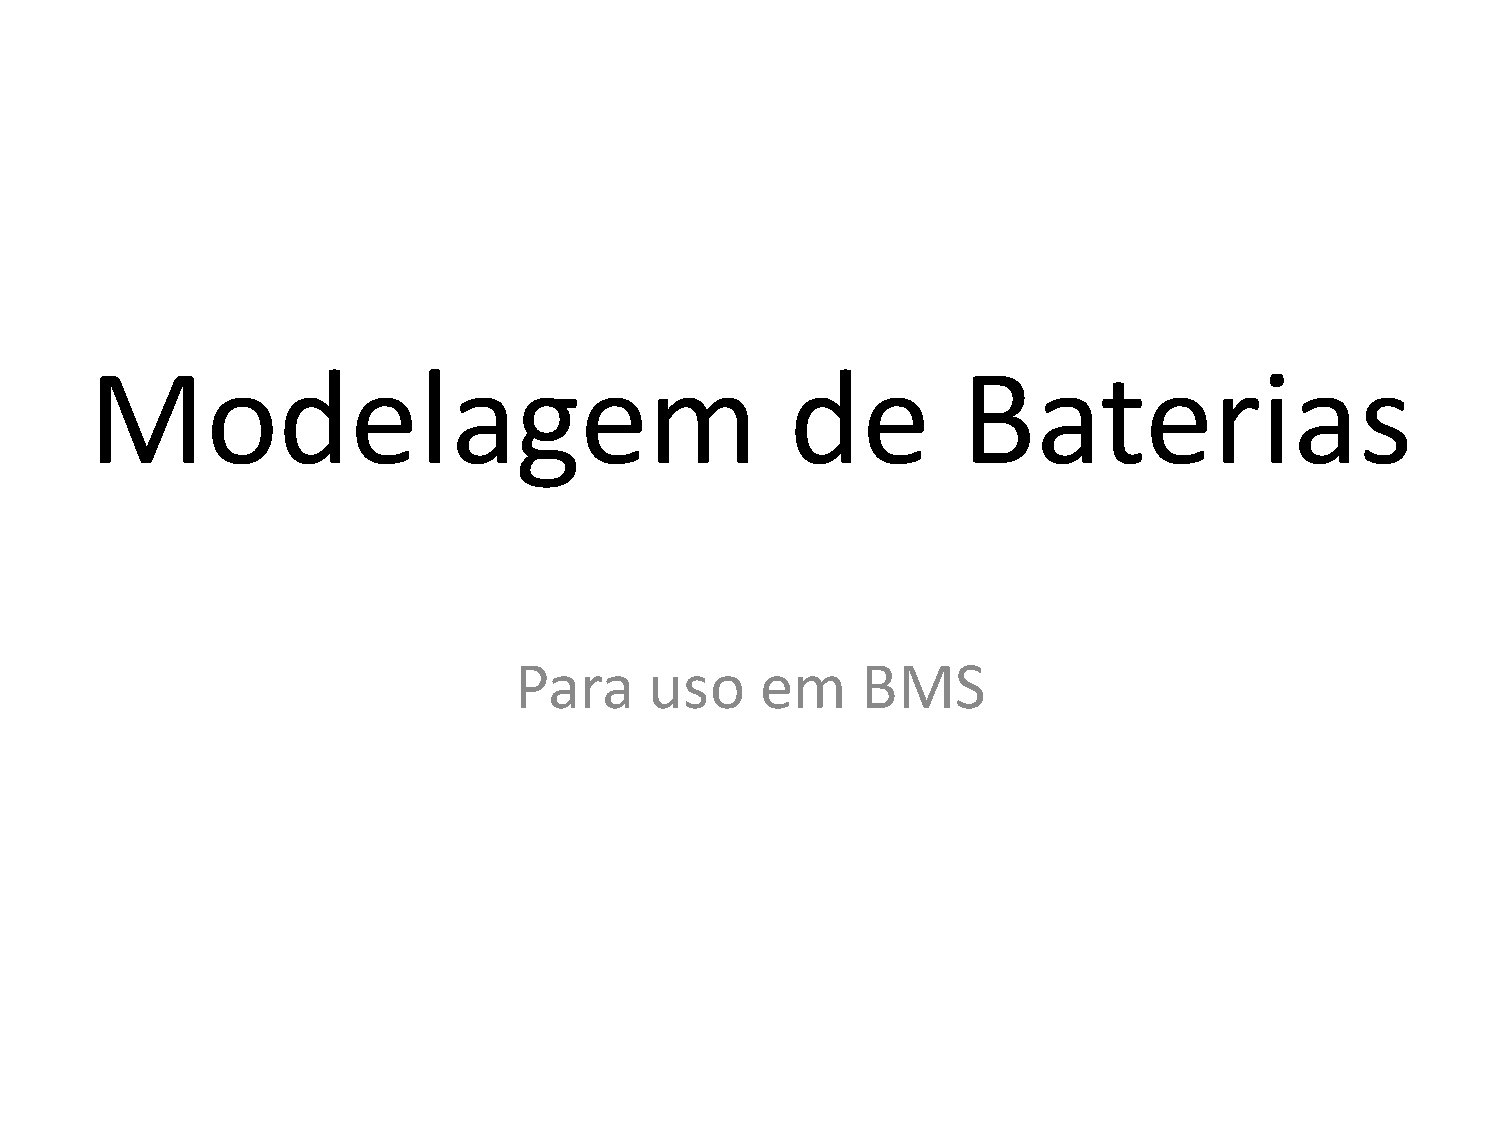
\includepdf[width=\textwidth,pages=-]{anexos/Modelagem_Baterias.pdf}

\begin{center}
  ~\vfill
  \framebox{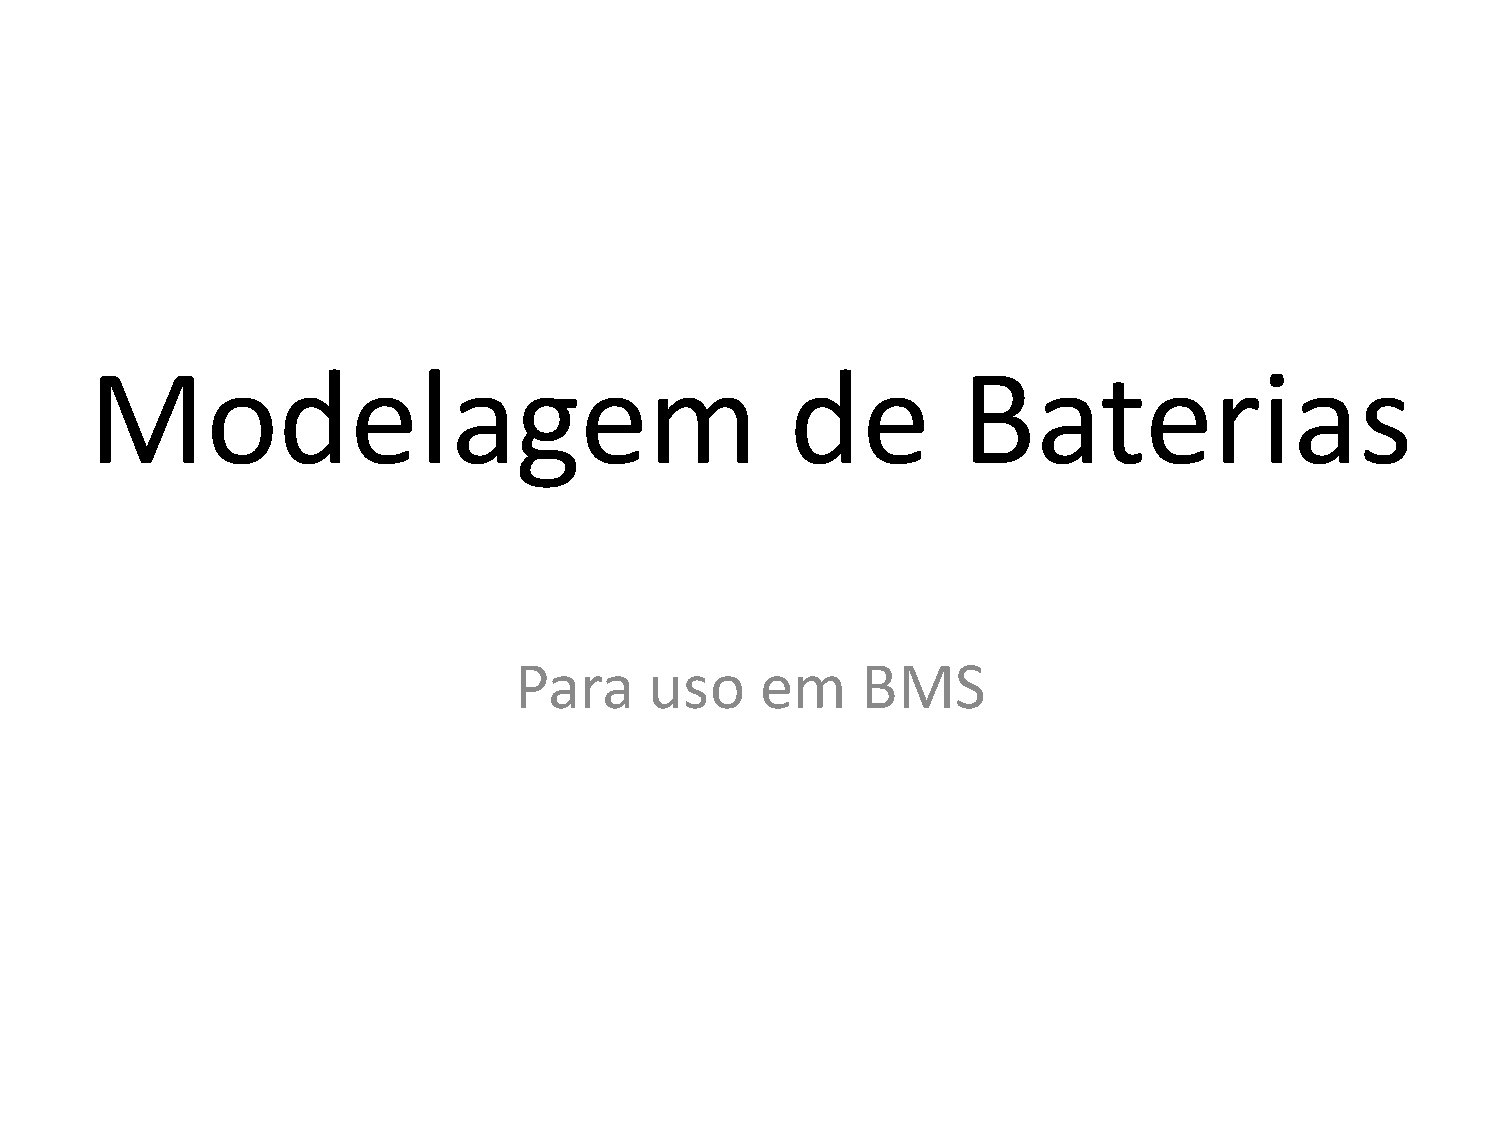
\includegraphics[scale=0.5]{anexos/Modelagem_Baterias-1.pdf}}
  \vfill
  \framebox{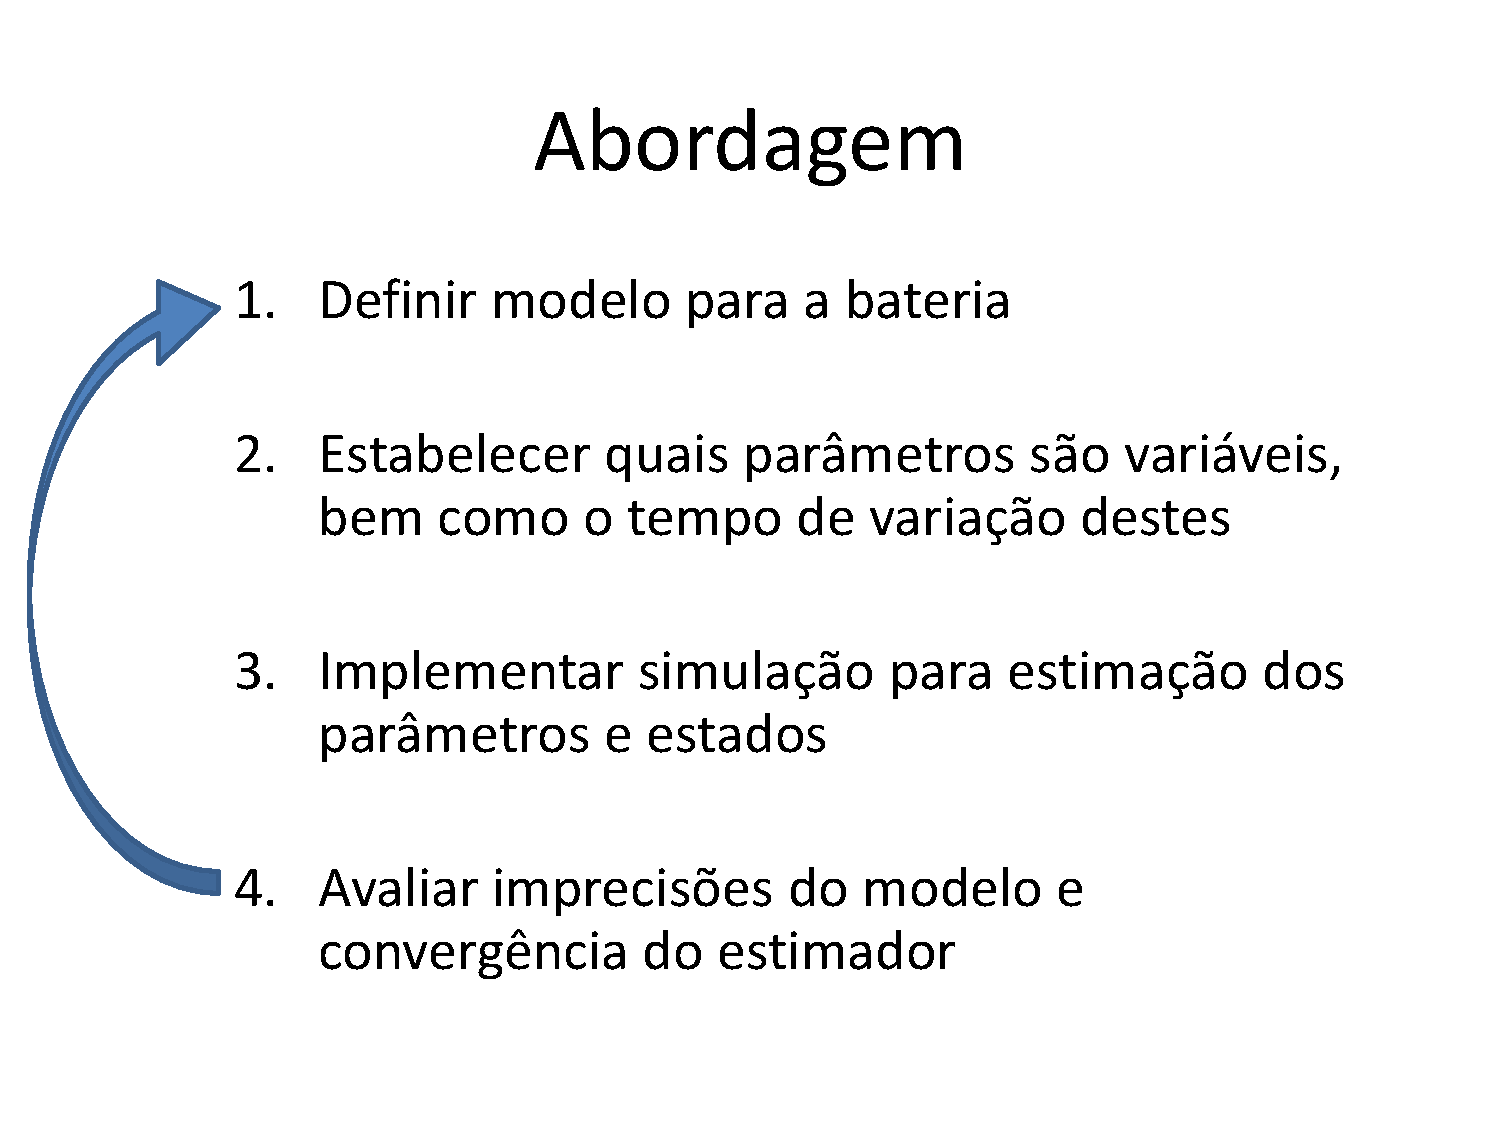
\includegraphics[scale=0.5]{anexos/Modelagem_Baterias-2.pdf}}
   \vfill
\newpage%
  ~\vfill
  \framebox{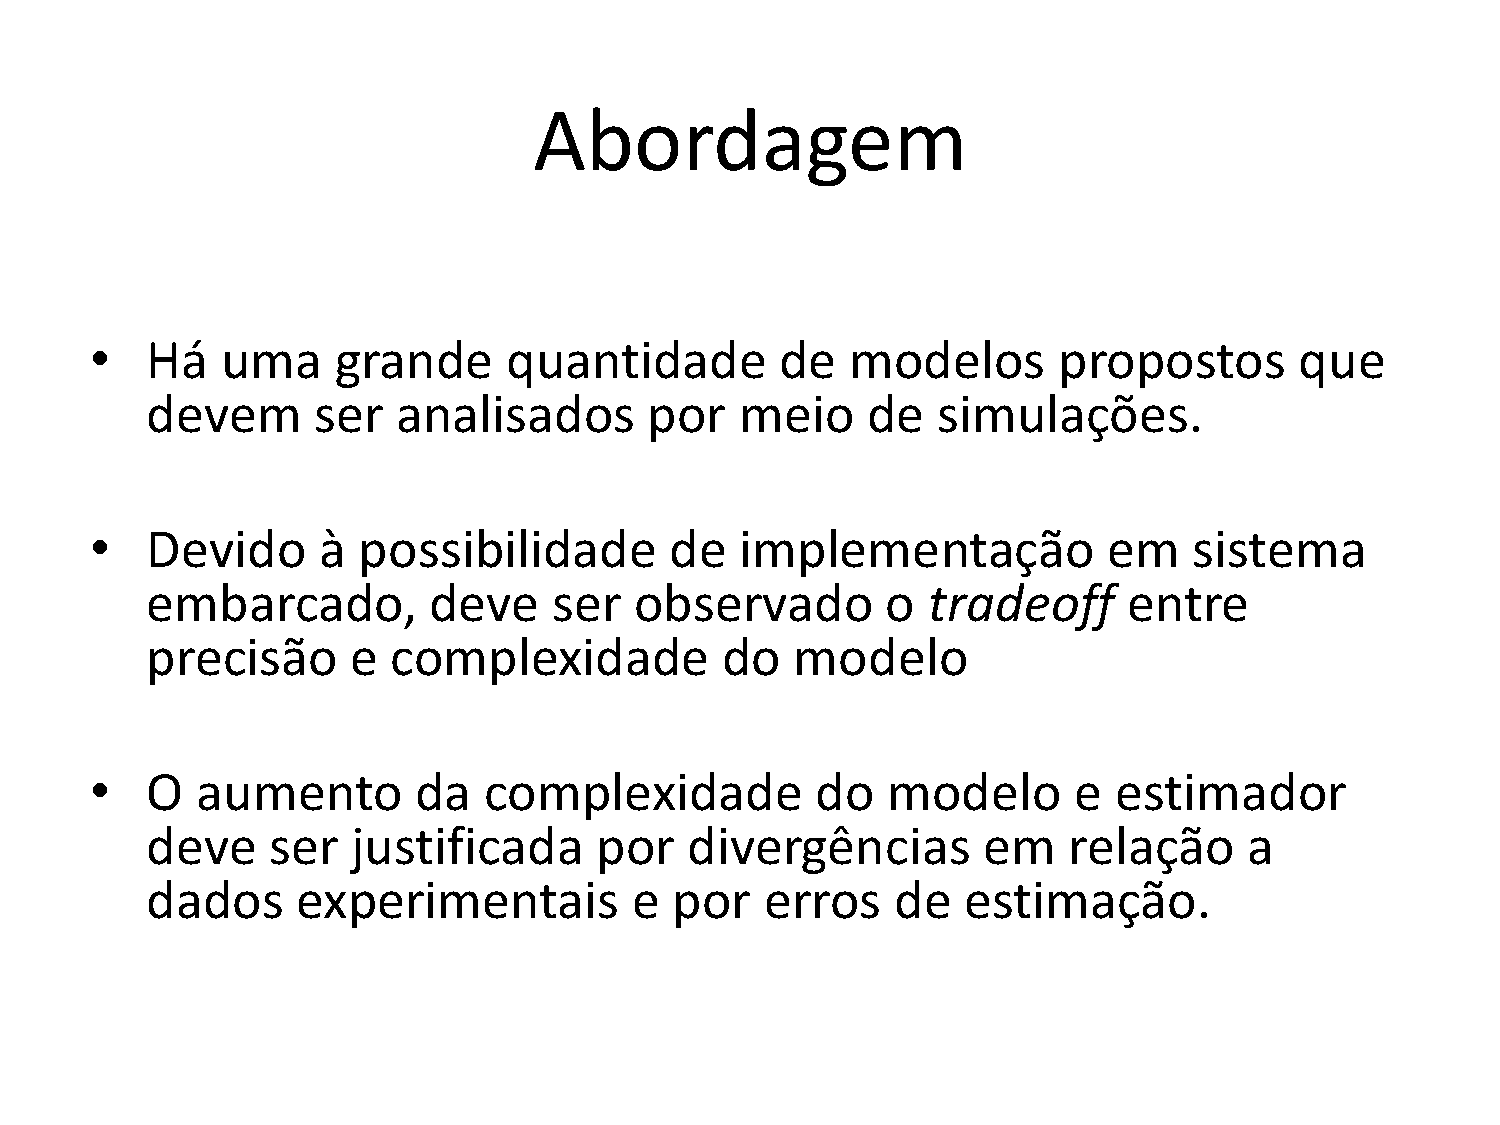
\includegraphics[scale=0.5]{anexos/Modelagem_Baterias-3.pdf}}
  \vfill
  \framebox{
\includegraphics[scale=0.5]{anexos/Modelagem_Baterias-4.pdf}}
   \vfill
\newpage%
  ~\vfill
  \framebox{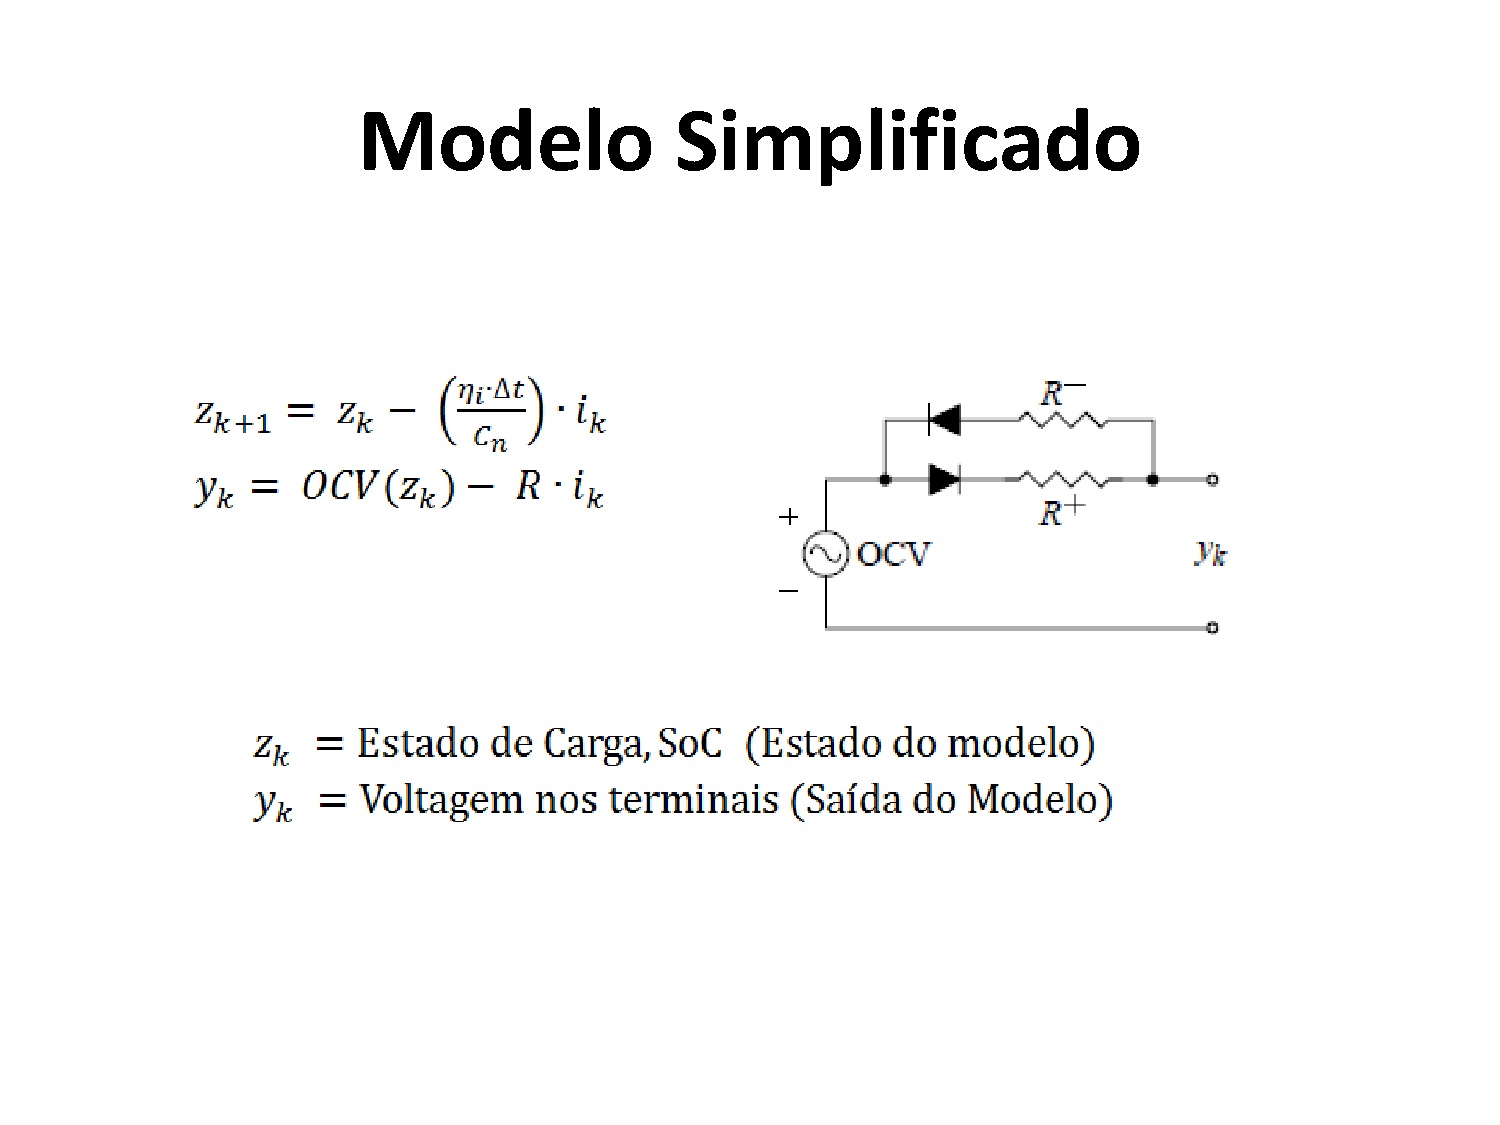
\includegraphics[scale=0.5]{anexos/Modelagem_Baterias-5.pdf}}
  \vfill
  \framebox{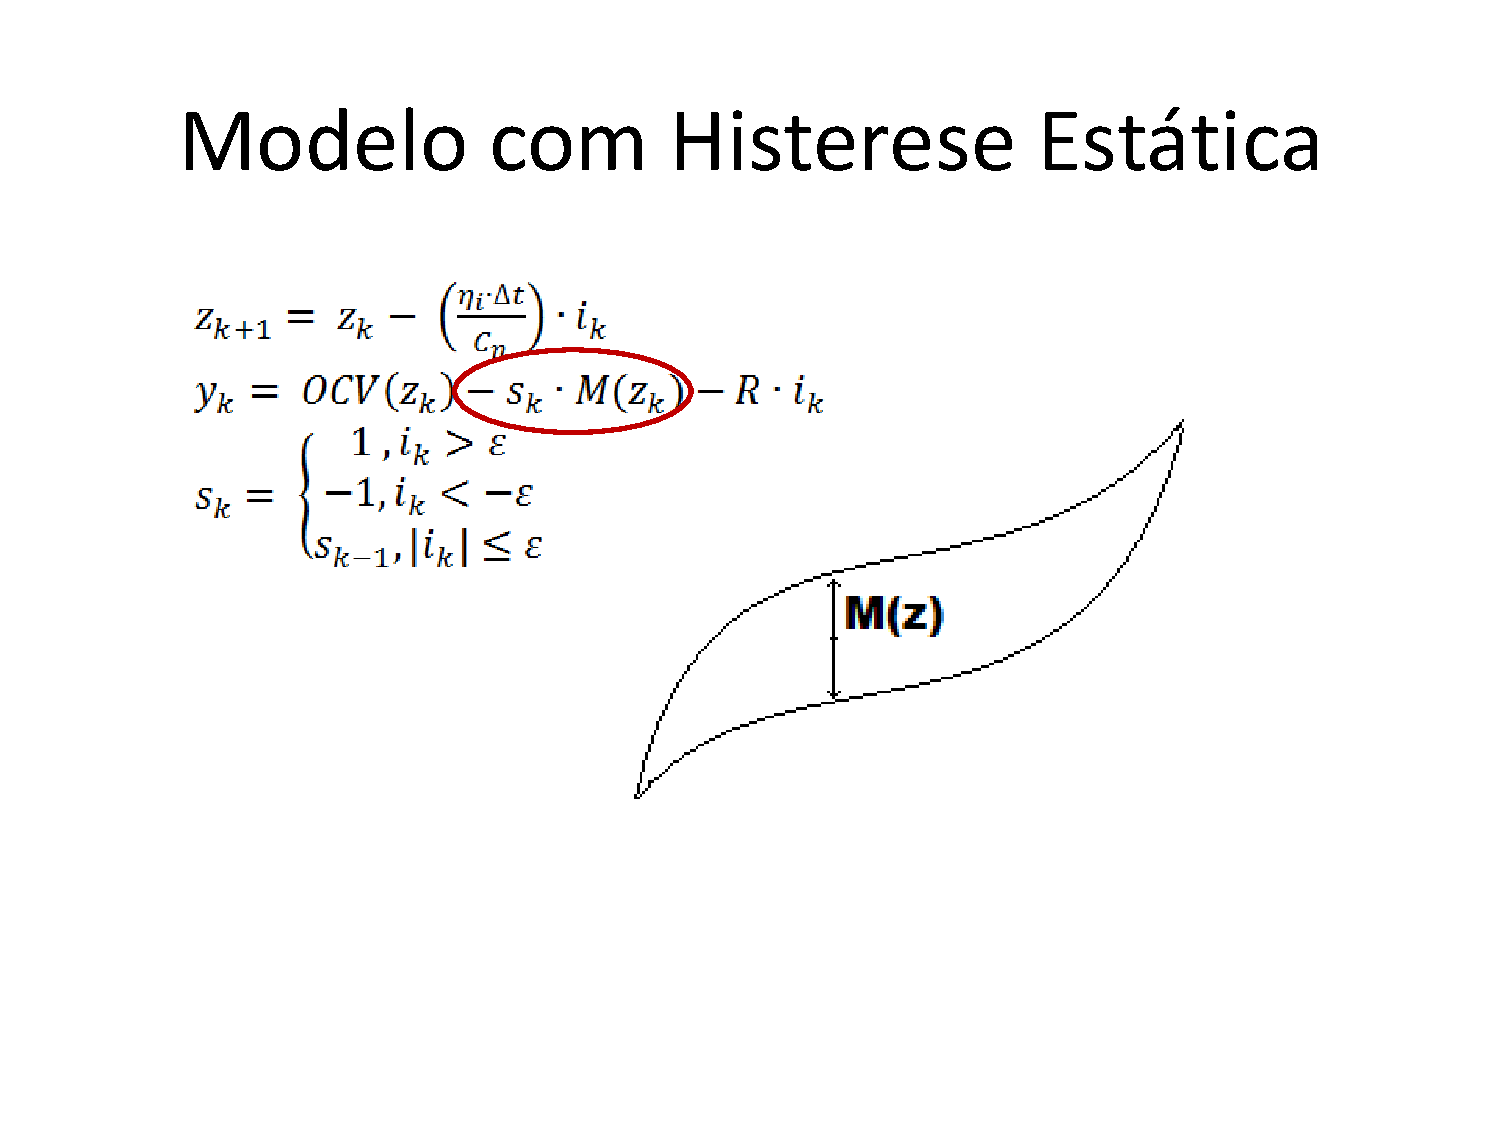
\includegraphics[scale=0.5]{anexos/Modelagem_Baterias-6.pdf}}
   \vfill
\newpage%
  ~\vfill
  \framebox{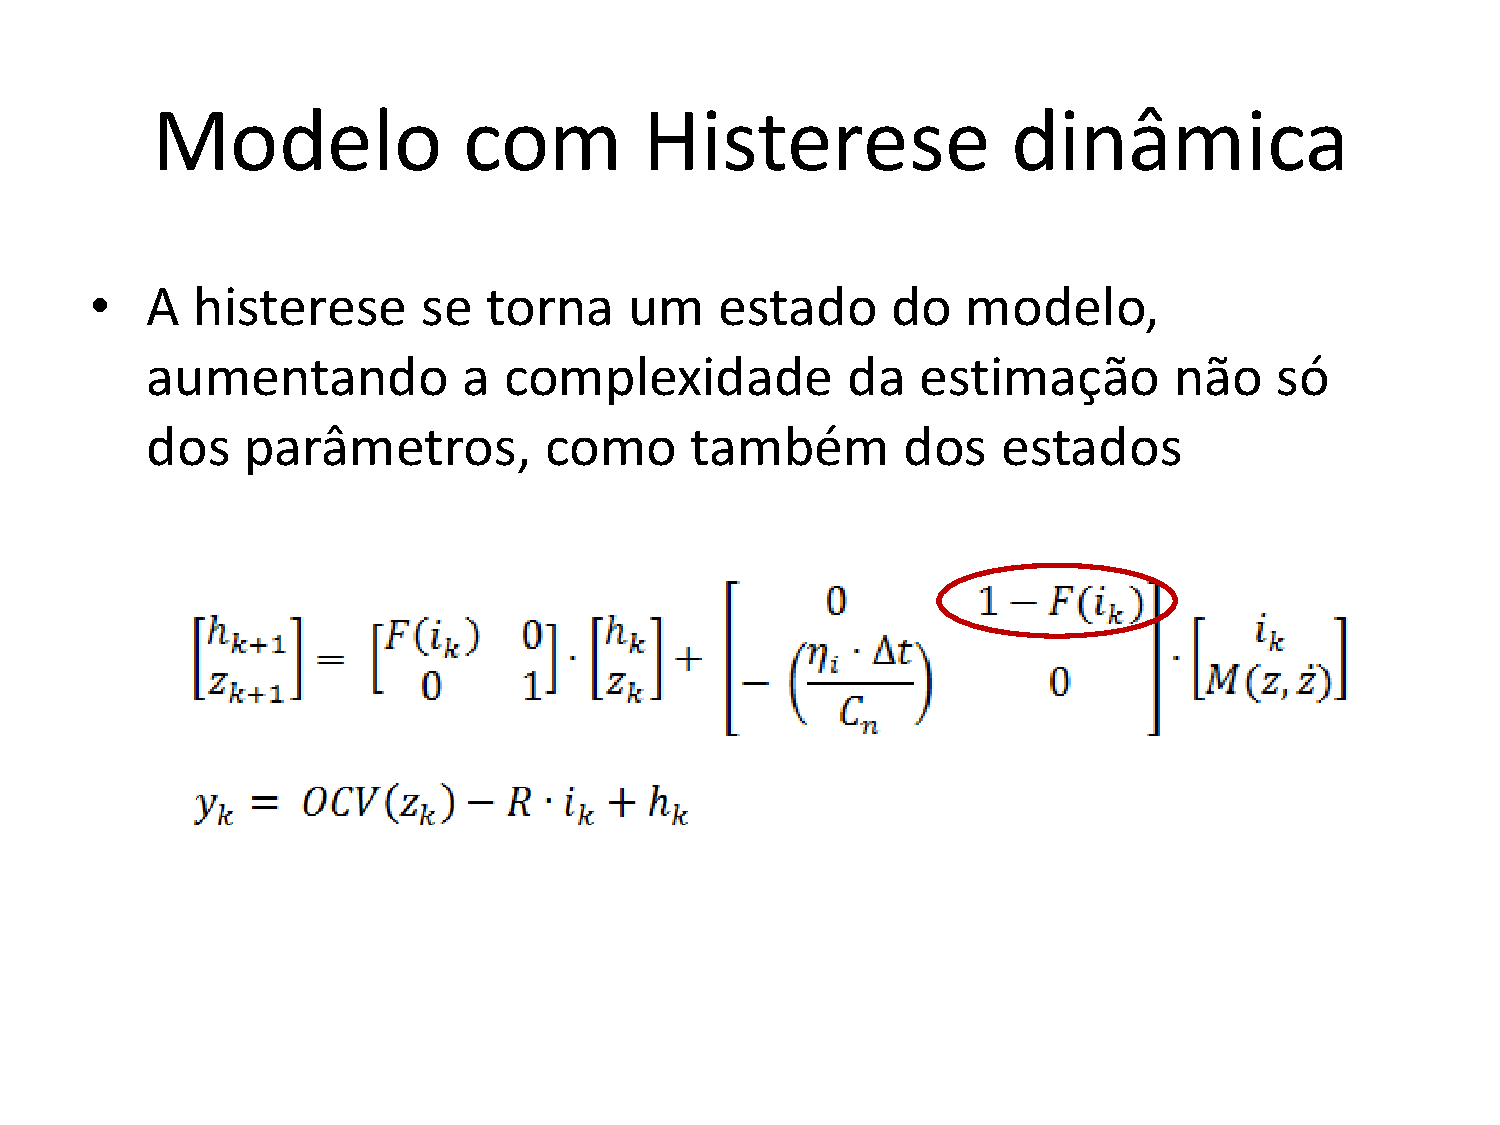
\includegraphics[scale=0.5]{anexos/Modelagem_Baterias-7.pdf}}
  \vfill
  \framebox{
\includegraphics[scale=0.5]{anexos/Modelagem_Baterias-8.pdf}}
   \vfill
\newpage%
  ~\vfill
  \framebox{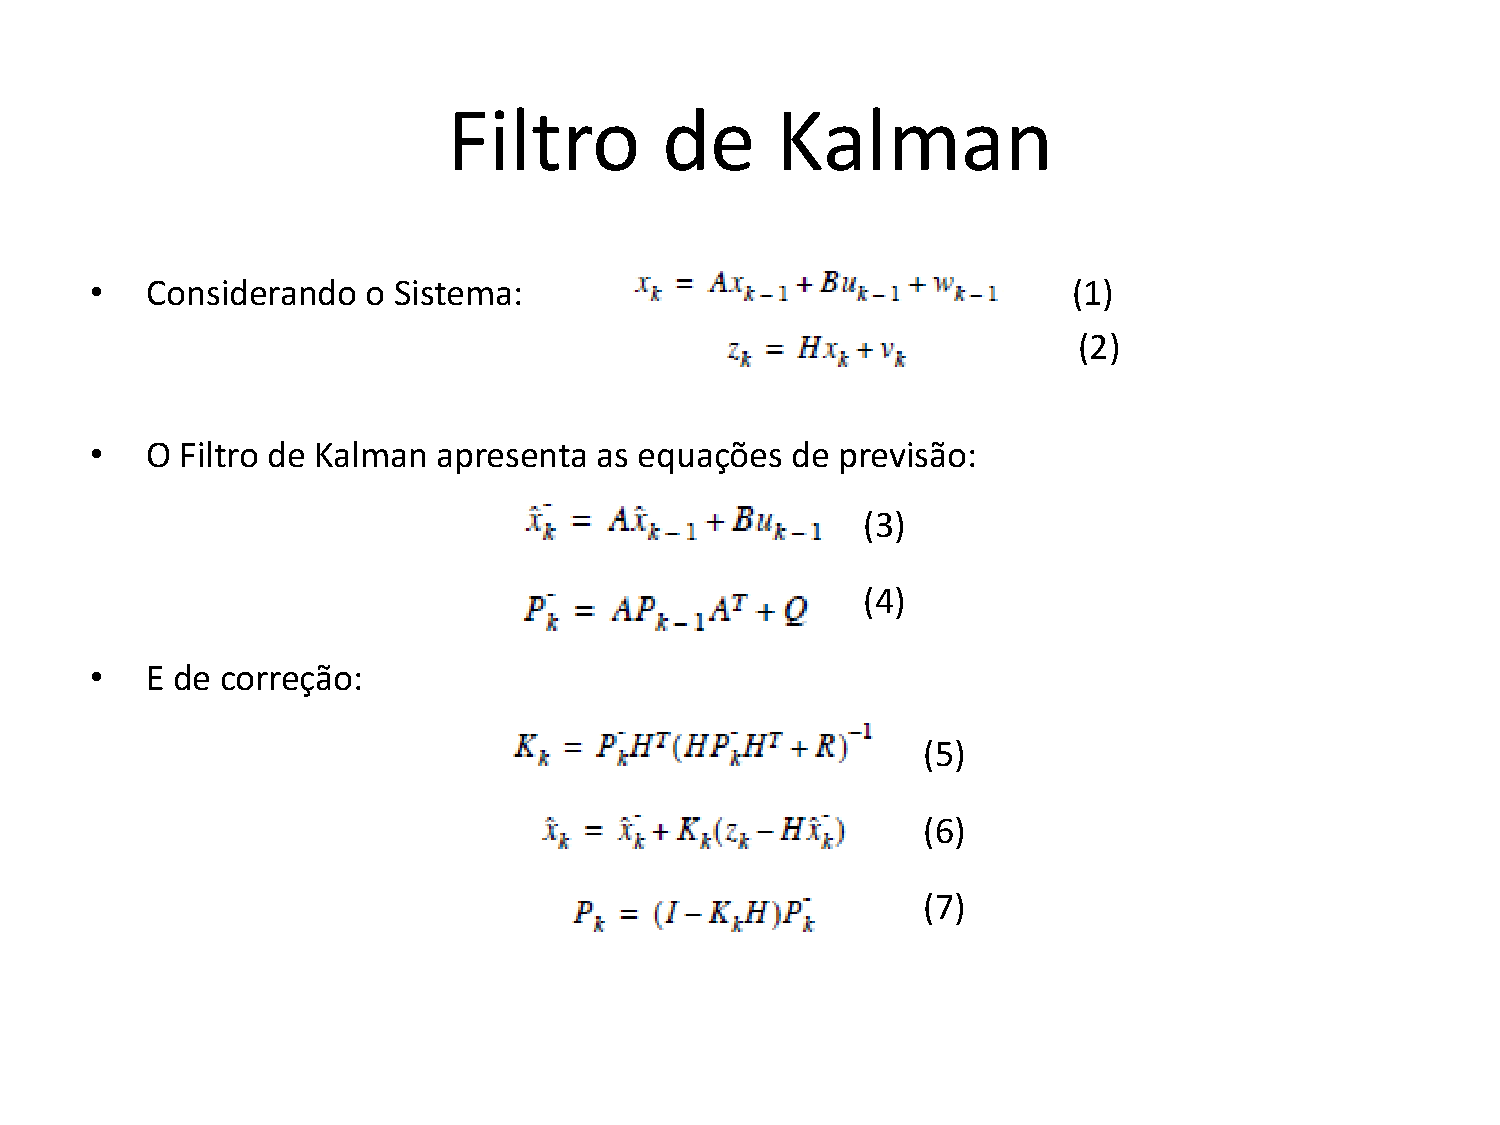
\includegraphics[scale=0.5]{anexos/Modelagem_Baterias-9.pdf}}
  \vfill
  \framebox{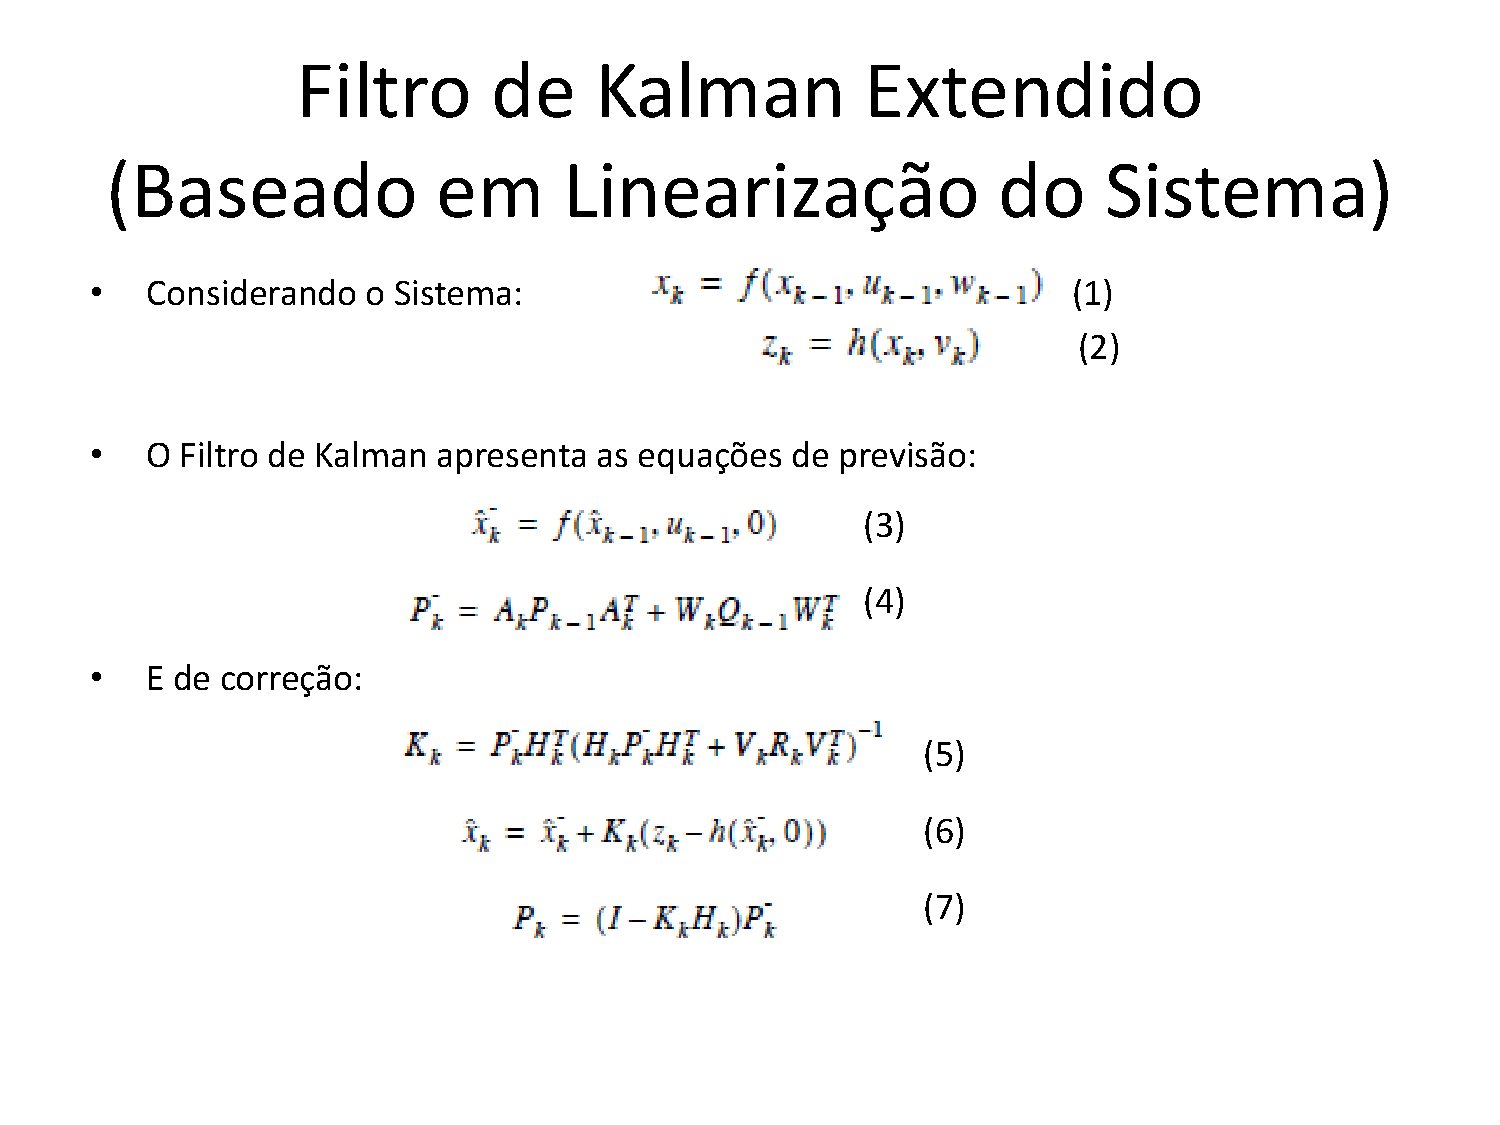
\includegraphics[scale=0.5]{anexos/Modelagem_Baterias-10.pdf}}
   \vfill
\newpage%
  ~\vfill
  \framebox{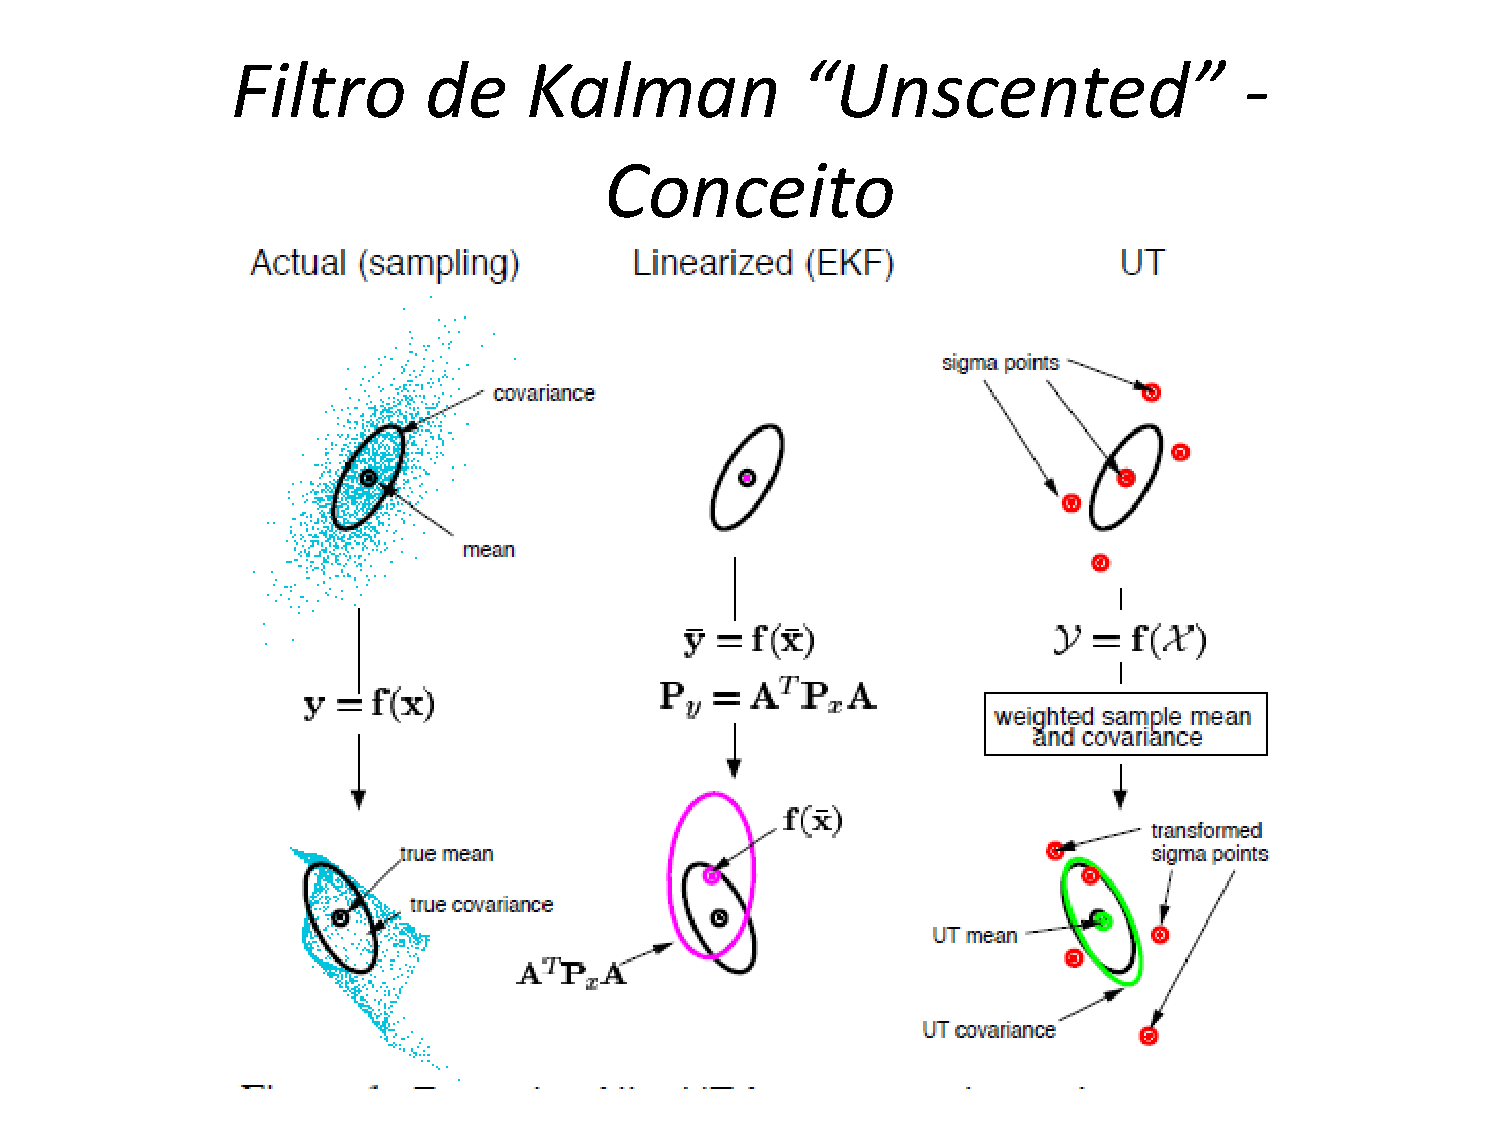
\includegraphics[scale=0.5]{anexos/Modelagem_Baterias-11.pdf}}
  \vfill
  \framebox{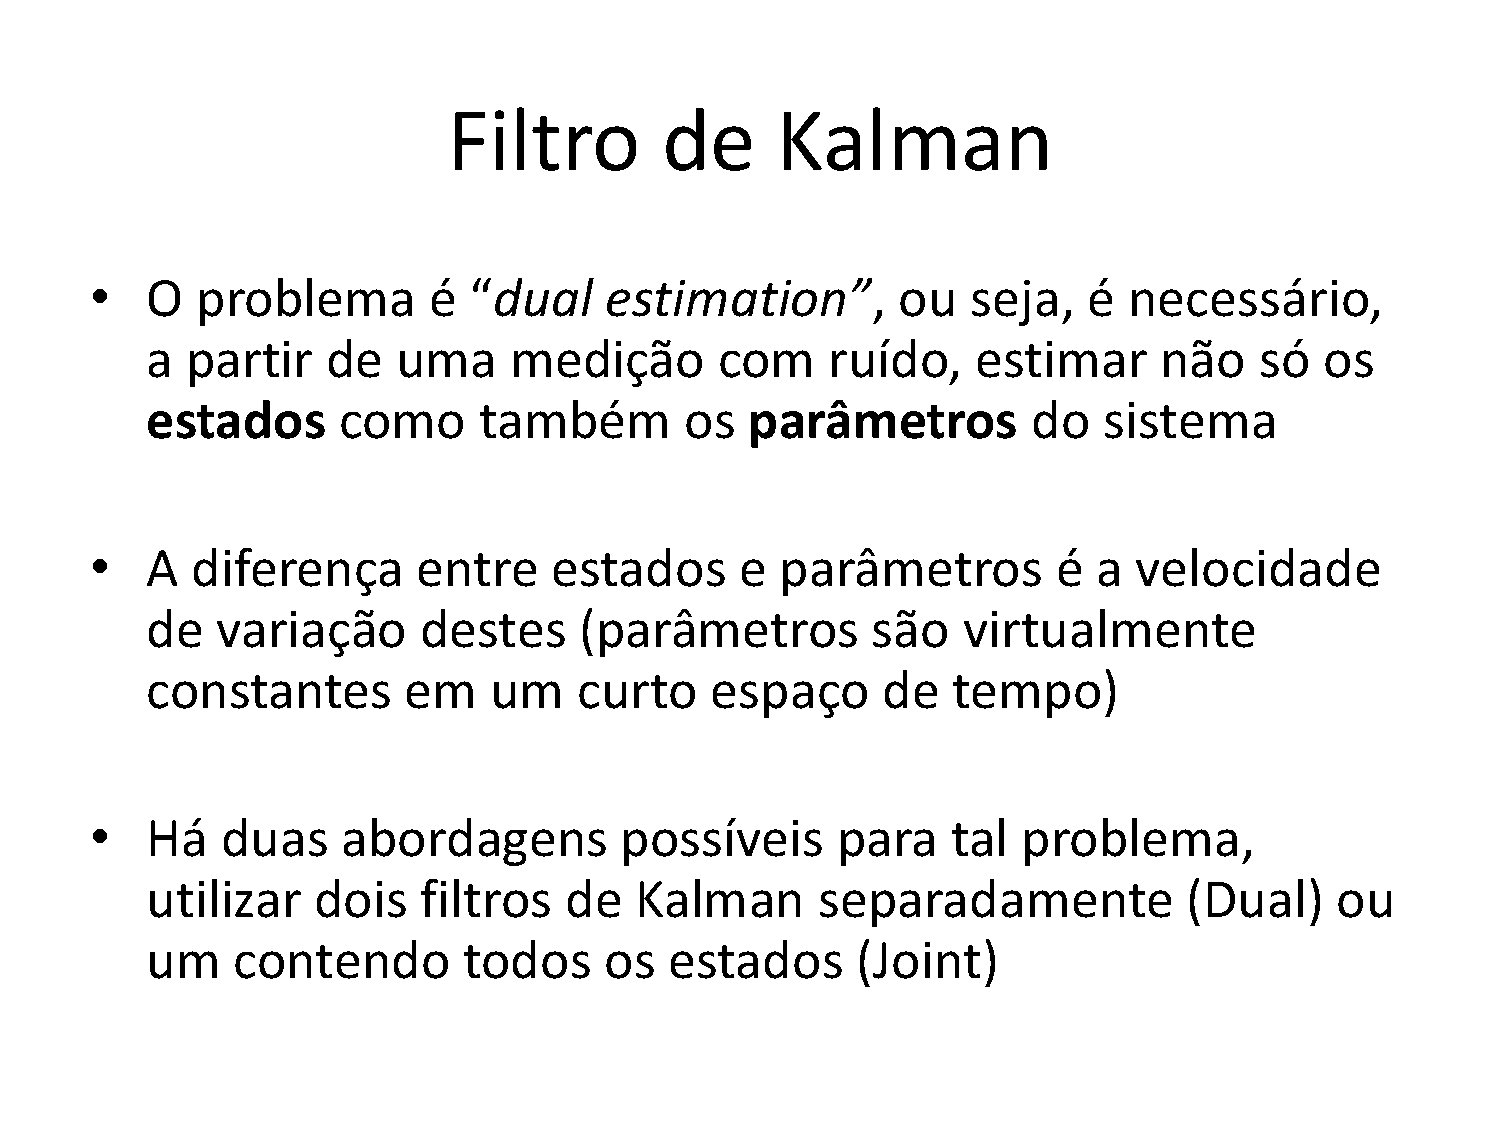
\includegraphics[scale=0.5]{anexos/Modelagem_Baterias-12.pdf}}
   \vfill
\newpage%
  ~\vfill
  \framebox{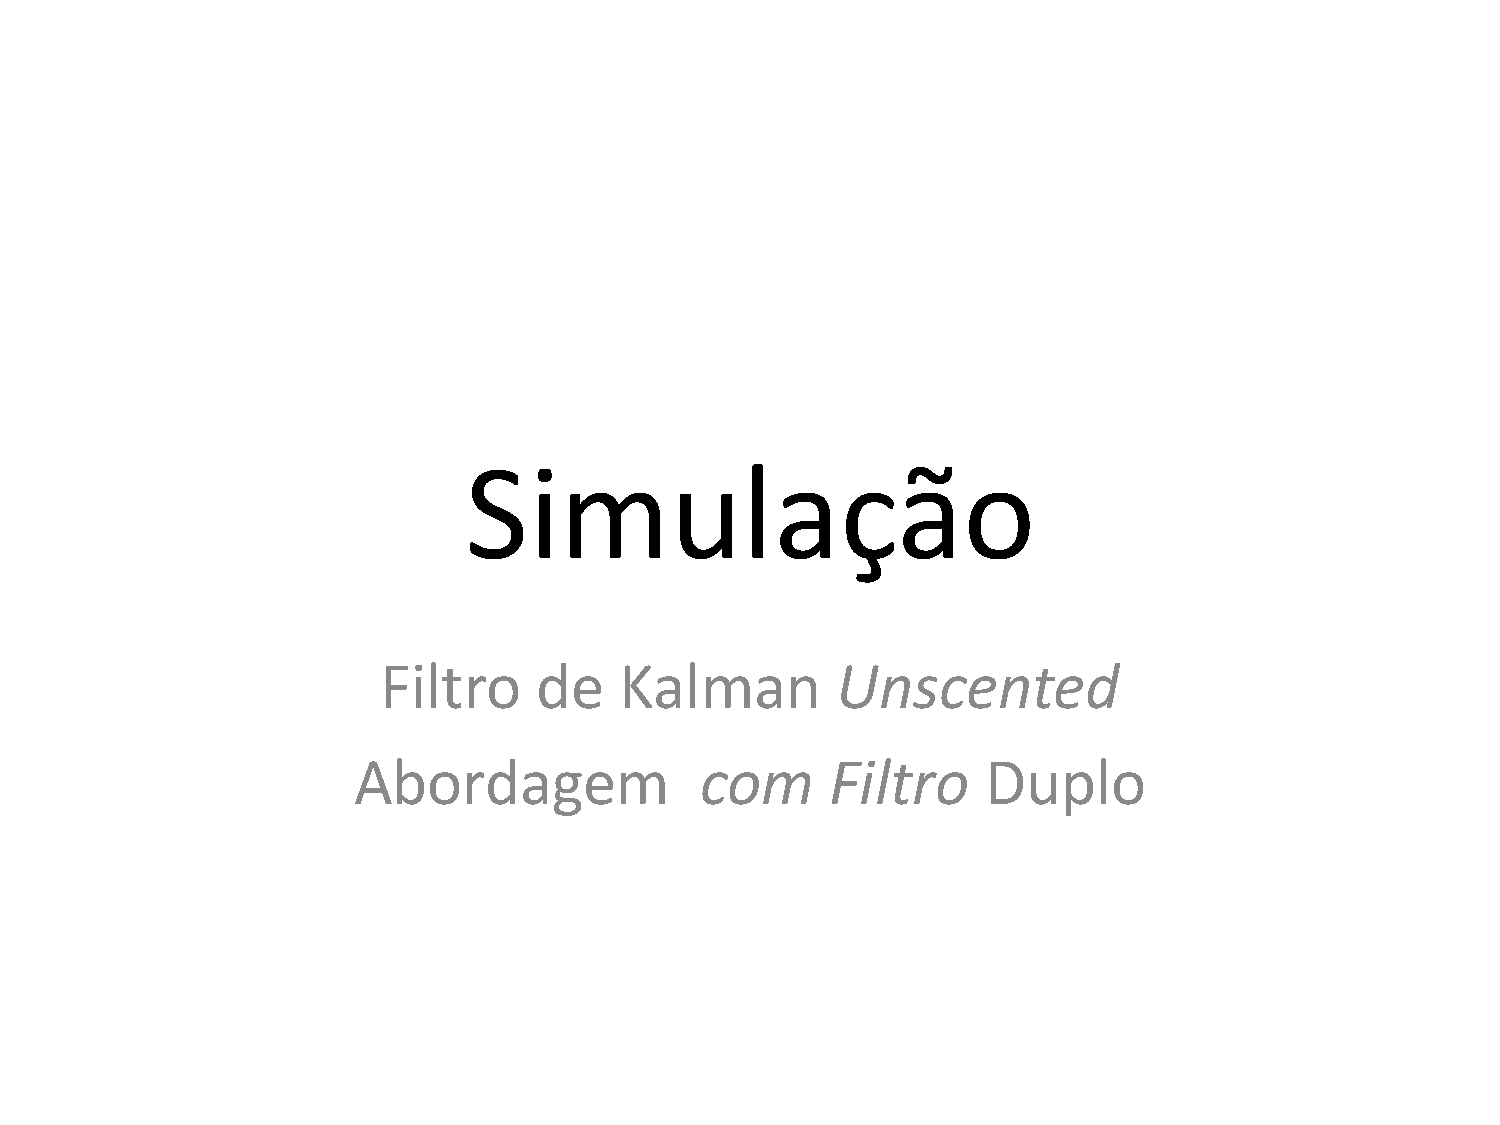
\includegraphics[scale=0.5]{anexos/Modelagem_Baterias-13.pdf}}
  \vfill
  \framebox{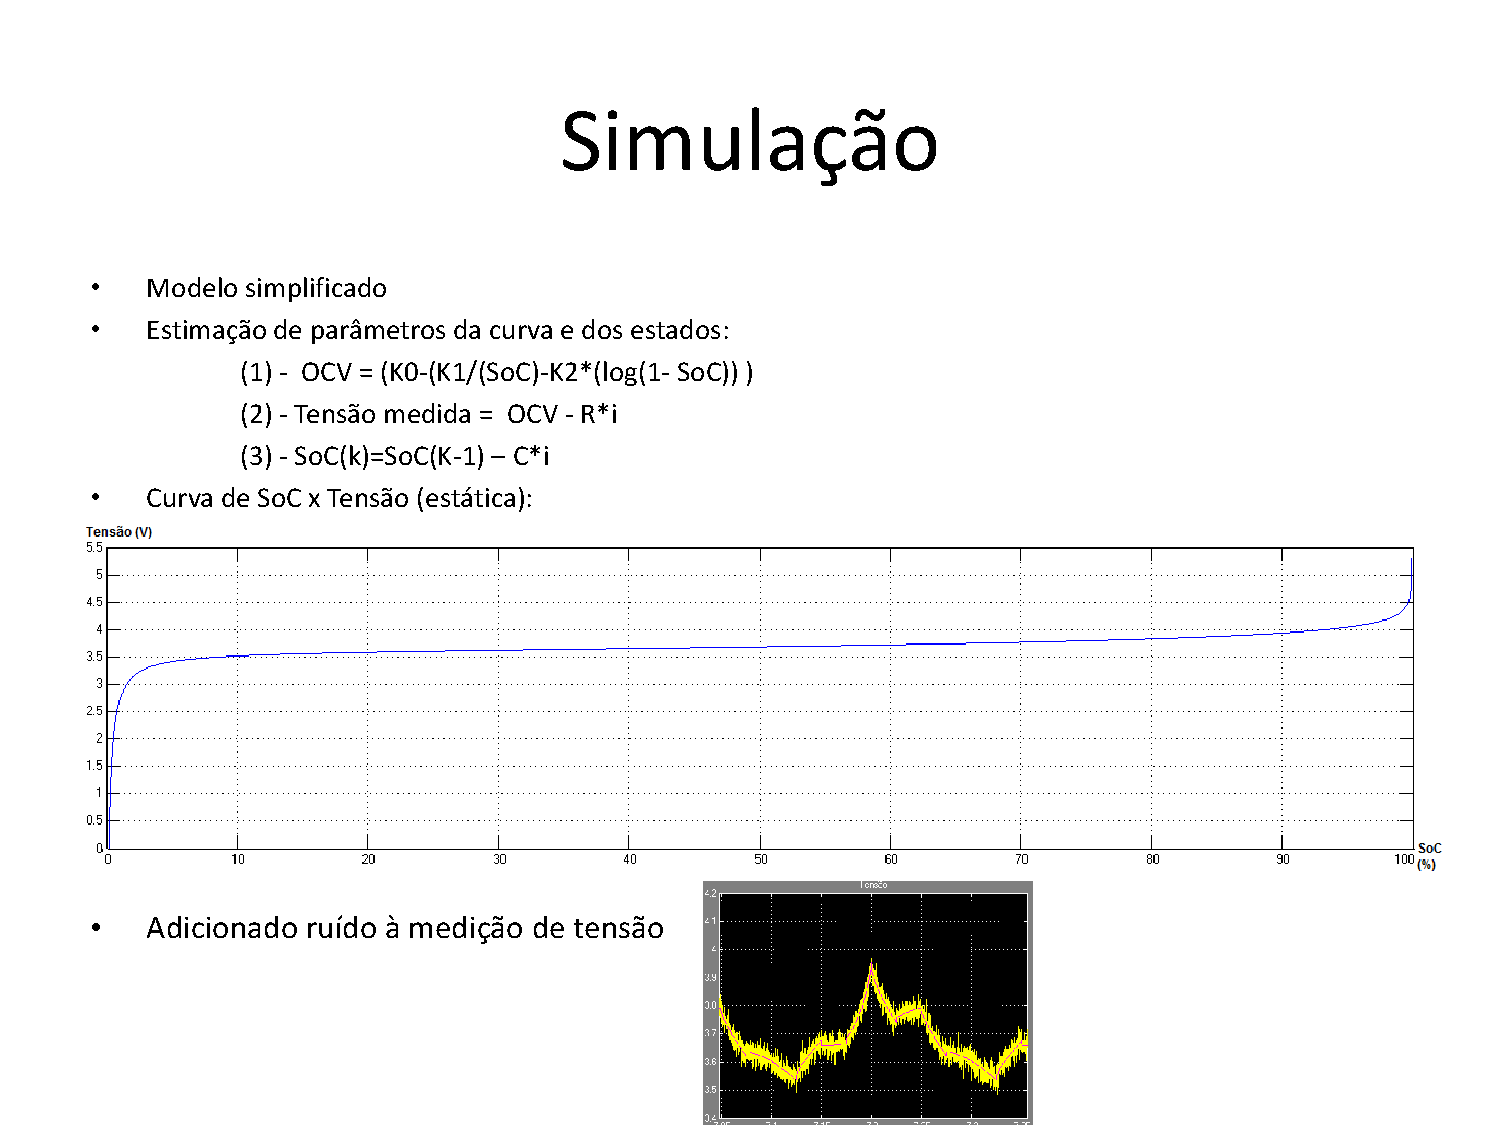
\includegraphics[scale=0.5]{anexos/Modelagem_Baterias-14.pdf}}
   \vfill
\newpage%
  ~\vfill
  \framebox{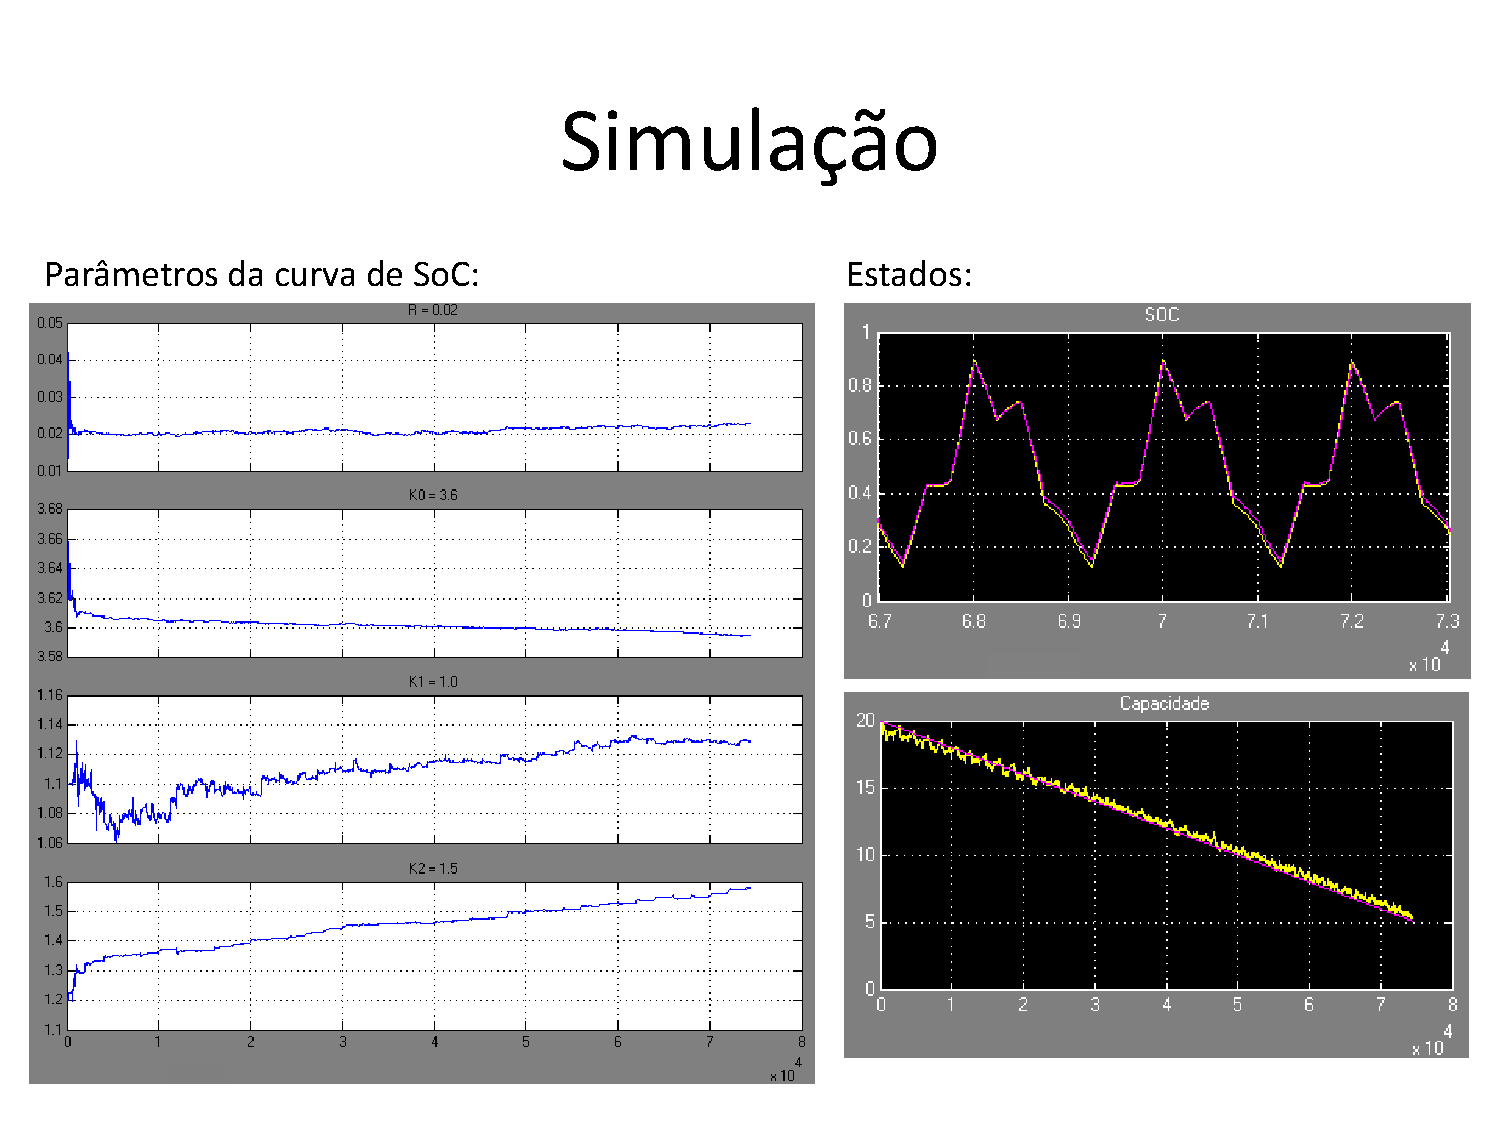
\includegraphics[scale=0.5]{anexos/Modelagem_Baterias-15.pdf}}
  \vfill
\newpage%
\end{center}








%\newpage%
%---------------------------------------------------------------------
%%% \section{Minutas}
%%%
%%% %---------------------------------------------------------------------
\subsubsection{Minuta de reuni�o (25-out-2013)}

\begin{tabbing}
  Local \= xxx \kill
  Local \> : LEAD \\
  Data  \> : 25 de Outubro de 2013 \\
  Hora  \> : 13:00
\end{tabbing}

%---------------------------------------------------------------------
\participantes{
  \jacoud,
  \andre,
  \elael,
  \julia,
  \patrick,
  \rafael,
  \ramon,
  \renan.
}

\begin{itemize}
  \item Update semanal. Resumo do que cada um estudou, as restri��es/recomenda��es e tarefas para a pr�xima semana.

  \begin{itemize}
    \item \textbf{\andre.} Estudou baterias e isolamento de cabos.
    Recomenda-se estudar sistemas de gerenciamento de pot�ncia e sincroniza��o dos equipamentos (time stamping).
    Pesquisar em ROV's: Sistemas de alimenta��o e umbilical. \\
    Nova Tarefa: Fazer um apanhado de possibilidades de sistemas de pot�ncia e umbilicais para saber qual se encaixaria melhor no projeto. \\

    \item \textbf{\rafael.} Novo bolsista de Mestrado. Tarefa preliminar: Explorar RockRobotics, familiarizar-se com a linguagem usada no projeto. \\
        Nova Tarefa: Instalar o ROCK, entender/familiarizar-se  com a programa��o do software e tentar resolver o primeiro exemplo do site. \\

    \item \textbf{\julia.} Trabalhando com identidade Visual, Planilha de aluguel Sylvain/ Invent�rio do Laborat�rio. \\
        Procedimentos de compras para o laborat�rio. \\
        Nova Tarefa: Site do projeto. Estrutura (perguntas, modelo, necessidades x usu�rios). Pesquisar sobre ROCK/Stoplogs, Pack Interface. \\
        Lembrete para Ramon: Contactar a acessoria de imprensa para divulgar o evento com a SBR em 3 de Nov. \\

    \item \textbf{\renan.} Foco em sensores de For�a. Fez pesquisa acessoria de forca, como os sensores funcionam, m�tricas importantes de mercado e o tipo de sensores que poder�amos usar no projeto. \\
        Nova Tarefa: Resumo de pros \& cons de sensores magn�ticos, focar em sensors a prova d'�gua.  Levantamento dos poss�veis m�todos para contato. Mini apresenta��o para ser discutida na semana que vem. \\

    \item \textbf{\elael.} Definido entre software e electr�nica, recomenda-se integra-lo no time de software que j� esta formado no LEAD. Estudou a documenta��o do ROCK.  \\
        Nova Tarefa: instalar o ROCK, entender/se familiarizar com a programa��o de software e tentar resolver o primeiro exemplo do site. Criar um drive. \\
  \end{itemize}

\end{itemize}

\vspace{10mm}%
\parbox[t]{70mm}{
  Aprovado por: \\[5mm]
  \centering
  %
\includegraphics[bb=1 1 1238 299,width=65mm]{../assinatura/assinatura-digital.jpg} \\[-4mm]
  
\includegraphics[width=65mm]{../assinatura/assinatura-digital.jpg} \\[-4mm]
  \rule[2mm]{70mm}{0.1mm} \\
  \ramon \\[1mm]
  Coordenador do Projeto \\
}

%---------------------------------------------------------------------
\fim


 \newpage%
%%% %---------------------------------------------------------------------
\subsubsection{Minuta de reuni�o (01-nov-2013)}

\begin{tabbing}
  Local \= xxx \kill
  Local \> : LEAD \\
  Data  \> : 01 de Novembro de 2013 \\
  Hora  \> : 13:00
\end{tabbing}

%---------------------------------------------------------------------
\participantes{
  \jacoud,
  \andre,
  \elael,
  \gabriel,
  \julia,
  \patrick,
  \rafael,
  \ramon,
  \renan.
}

\begin{itemize}
  \item Aprova��o da minuta.

  \item Discutir tarefas e recomenda��es da equipe para essa semana.

  \item Viagem a Porto Velho, Energia Sustent�vel do Brasil, adiada para o dia 10/11/2013.

  \item Update semanal. O que cada um do grupo desenvolveu durante a semana.
  \begin{itemize}
    \item \textbf{\andre.} N�o teve condi��o de pesquisar. Tarefa mantida para semana que vem. \\
        Tarefa: Pesquisa de possibilidades de sistemas de pot�ncia umbilical que se encaixem no projeto. \\

    \item \textbf{\rafael.} Cumpriu tarefa, instalou ROCK e fez o exerc�cio, familiarizando-se com a linguagem, criando drivers e library. \\

    \item \textbf{\julia.} Criative brief CIR. Atualizou planilhas de invent�rios e aluguel/ rockrobotics.org/ interface Package/reuni�o com professor Cl�udio Esperan�a/ Doris Kominsky. \\ Tarefas: criar o modelo do nosso site/ aulas de phyton/ computer logics (gradua��o) com Cl�udio Esperan�a. \\

    \item \textbf{\renan.} Apresentou pros \& cons de sensores magn�ticos e a prova d'�gua e fez um levantamento de poss�veis sensores e respectivos m�todos para contato. Garras atuadas. \\
        Tarefa: Sketch do equipamento inicial necess�rio, levantamento de sensor indutivo, camera guppy. Pesquisar a resist�ncia do a�o/underwater pump. \\

    \item \textbf{\elael.} Cumpriu tarefa. Encontrou alguns problemas de instala��o mas junto com o grupo de programa��o criou driver e explorou a linguagem. Tamb�m criou uma interface b�sica de controle usando Ruby. \\
        Tarefa: Tentar implementar sensors utilizados no ROCK. \\

    \item \textbf{\gabriel.} Cumpriu tarefa, encontrou alguns problemas de instala��o mas junto com o time de programa��o criou driver e explorou a linguagem. Quer relacionar o projeto com apresenta��o de aula de redes neurais. \\
        Tarefa: \\
  \end{itemize}

  \item Problemas em aberto:
  \begin{itemize}
    \item Procedimento de compras e medidas para as instala��es finais do laborat�rio.
    \item Op��es para a comprar de software, Adobe/ Solid Works/ Live Meeting/Bibliografia
    \item Fechar or�amento Invent�rio.
    \item Criar log para documentar problemas de ROCK/ criar um forum para colabora��o (?!)
    \item Dropbox para compartilhamento de arquivos.
    \item Viagem ESB/Relat�rio:
    \begin{itemize}
      \item Verificar encaixe (medi��o, propor��es) dos ganchos durante a visita a ESB para determinar que tipos de sensores podem ser implementados.
      \item Modelo detalhado do processo + Blueprints. \\
    \end{itemize}
  \end{itemize}

  \item Agenda para a pr�xima reuni�o:
  \begin{itemize}
    \item Resultado de pesquisas individuais.
    \item Relat�rio de viagem.
    \item Novas tarefas \& recomenda��es.
  \end{itemize}

\end{itemize}

\vspace{5mm}%
\parbox[t]{70mm}{
  Aprovado por: \\[5mm]
  \centering
  \includegraphics[width=65mm]{../assinatura/assinatura-digital.jpg} \\[-4mm]
  \rule[2mm]{70mm}{0.1mm} \\
  \ramon \\[1mm]
  Coordenador do Projeto \\
}

%---------------------------------------------------------------------
\fim


 \newpage%

%---------------------------------------------------------------------
\fim

%---------------------------------------------------------------------
\end{document}
